%%
%% Author: Dario Chinelli
%% begin 2019-12-04
%% last mod 2022-02-02
%%

% Preamble
\documentclass[class=article, crop=false]{standalone}

% Packages
\usepackage[subpreambles=true]{standalone}
\usepackage{import}
\usepackage{graphicx}
\usepackage{amsmath}

% Document
\begin{document}
The aim of this paragraph is the comparison between the real dataset utilized to produce the models and some simulations.
The following quantities are taken into account to compare the results.
Those are plotted as histograms, to empathize the statistical approach.
\begin{enumerate}[label=(\roman*)]
\item The magnitude of the velocity vector along the $\vec x$ axes, plotted as 1-dimensional histogram;
\item the magnitude of the velocity vector along the $\vec y$ axes, plotted as 1-dimensional histogram;
\item the correlation between the position along the $\vec x$ axes and the magnitude of the velocity vector along the same axes, plotted as heat-map or 2-dimensional histogram;
\item the correlation between the position along the $\vec y$ axes and the magnitude of the velocity vector along the same axes, plotted as heat-map or 2-dimensional histogram.
\item the heat-map of the positions along $\vec x$ and $\vec y$ axis of all paths that have passed though, plotted as 2-dimensional histogram;
\end{enumerate}

\FloatBarrier
\subsection{Real data - D2Q9}
This paragraph's reference are the following: (Figure \ref{fig:hist_SimD2Q9}), (Figure \ref{fig:hist2d_SimD2Q9}), (Figure \ref{fig:Pxy_SimD2Q9}).


\begin{figure}[!htb]
    \centering
    \subfloat[(i) Real data hist vx]{
        \label{fig:Vx_Real_i}
        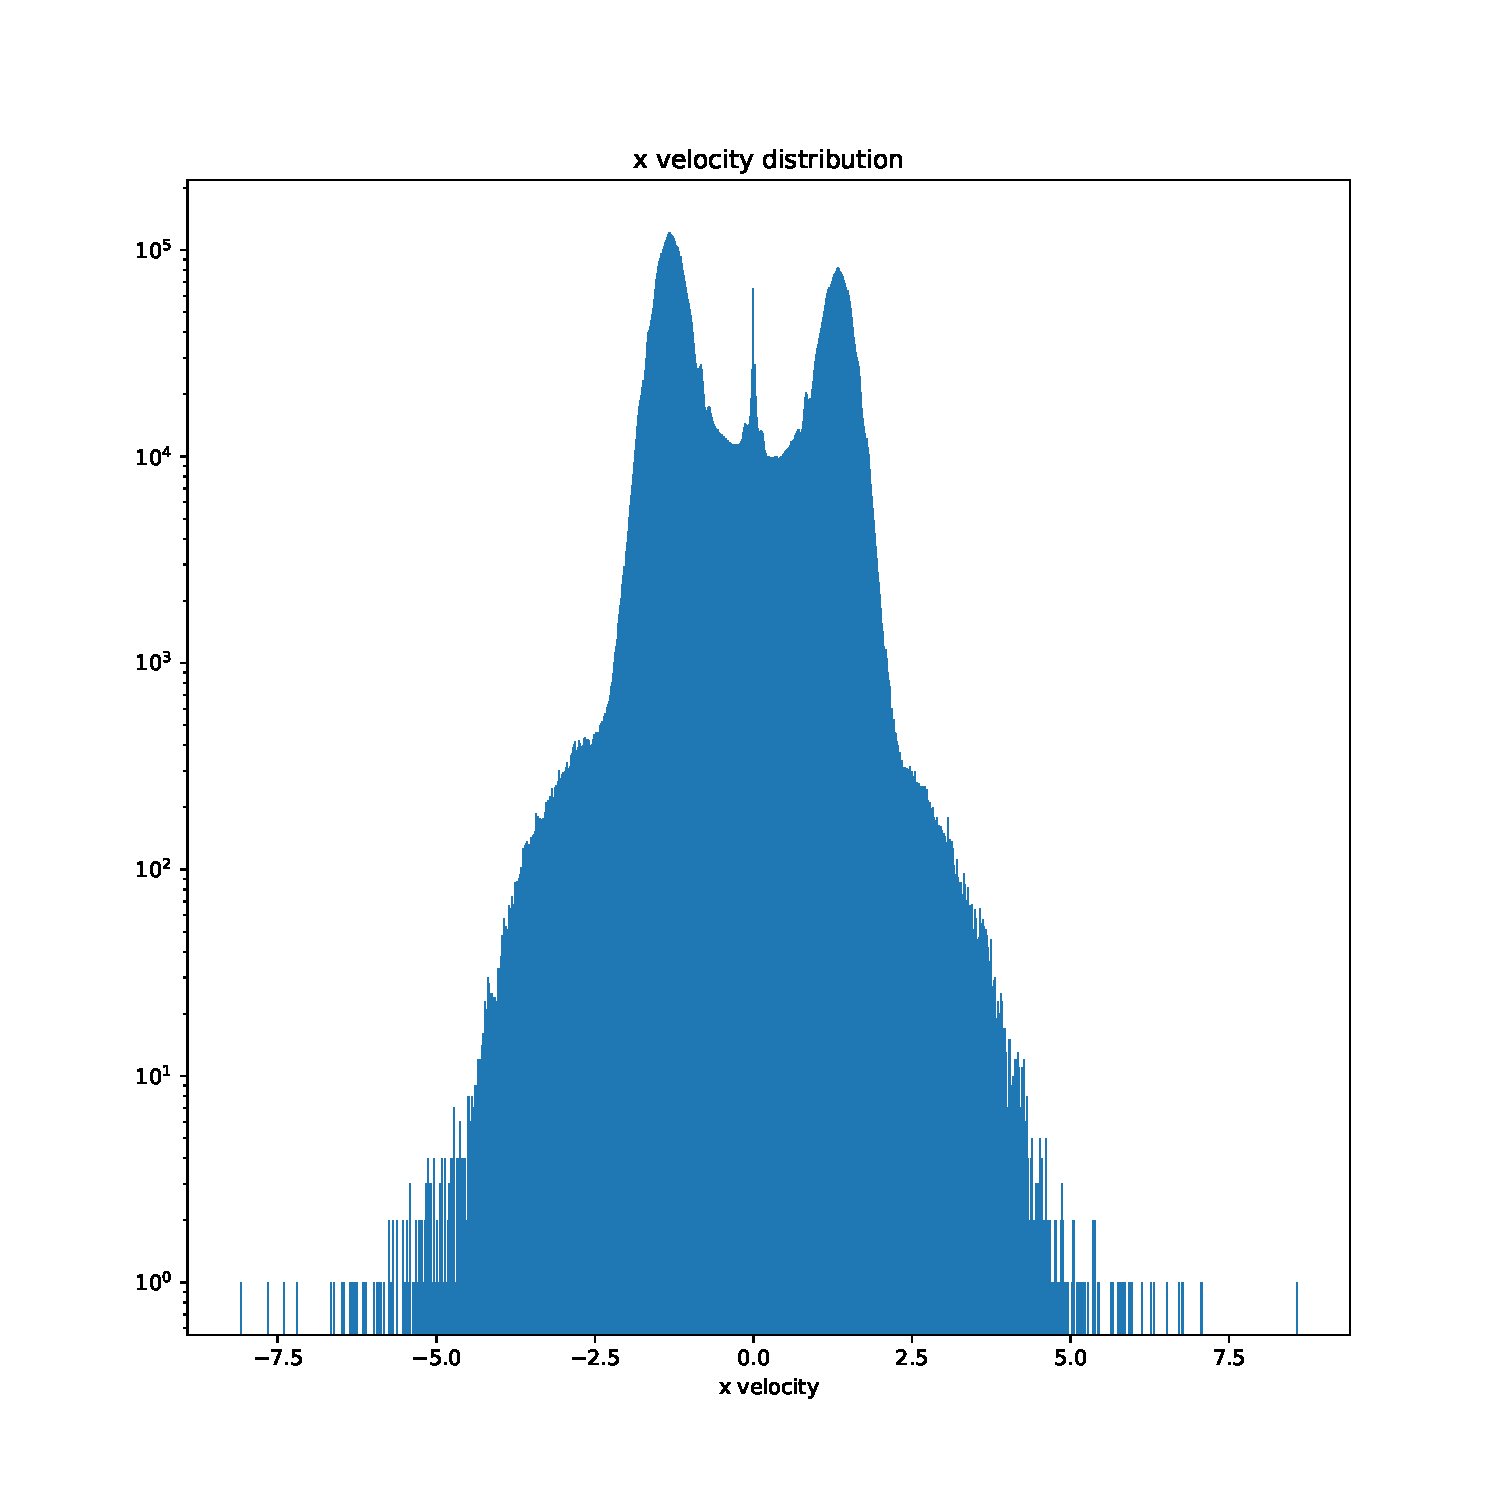
\includegraphics[ width=0.3\textwidth]{fig/hist_vx/save_trainf10_pro_RealData_hist_vx}
    }\quad\quad
    \subfloat[(i) Simulation data hist vx]{
        \label{fig:Vx_SimD2Q9}
        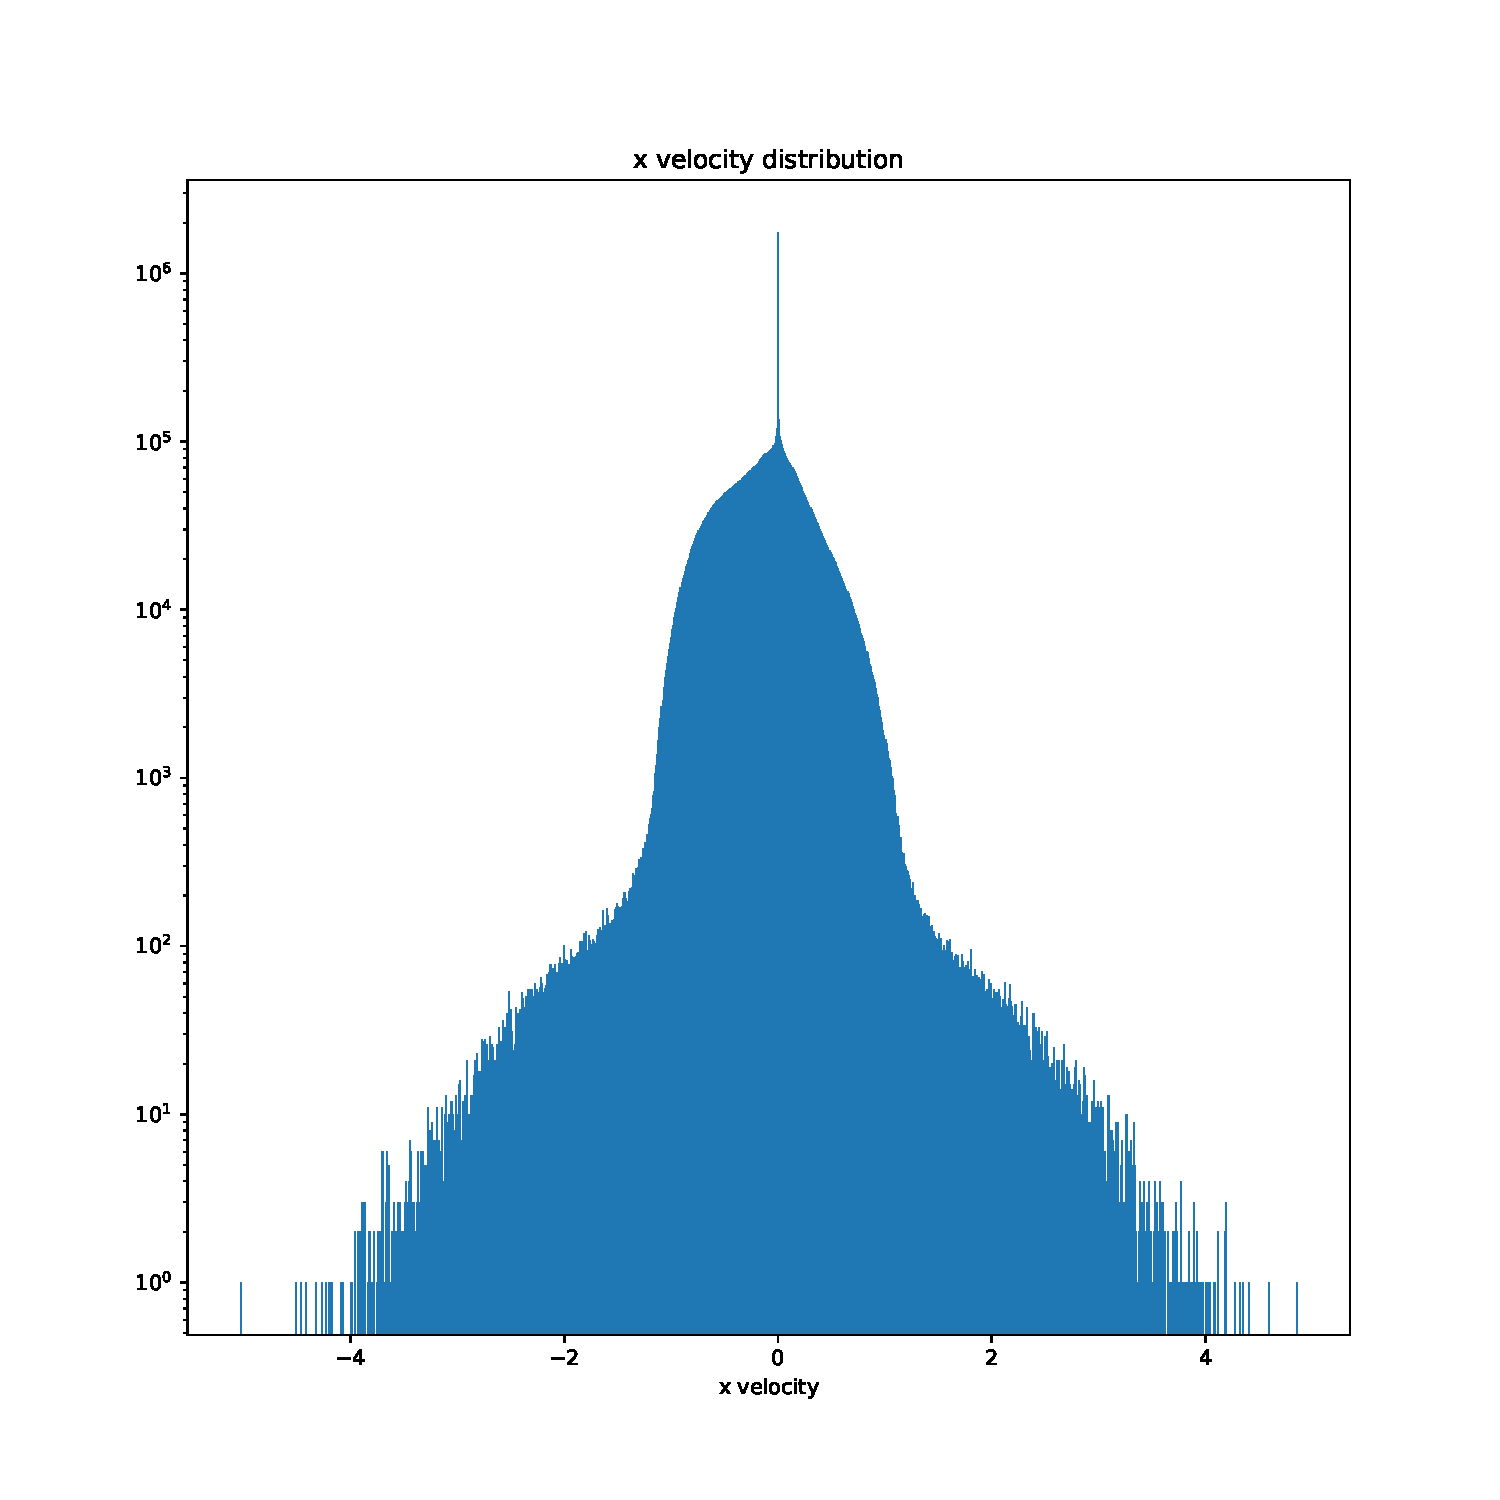
\includegraphics[ width=0.3\textwidth]{fig/hist_vx/save_trainf10_pro_simD2Q9_hist_vx}
    }\quad\quad
    \subfloat[(ii) Real data hist vy]{
        \label{fig:Vy_Real_ii}
        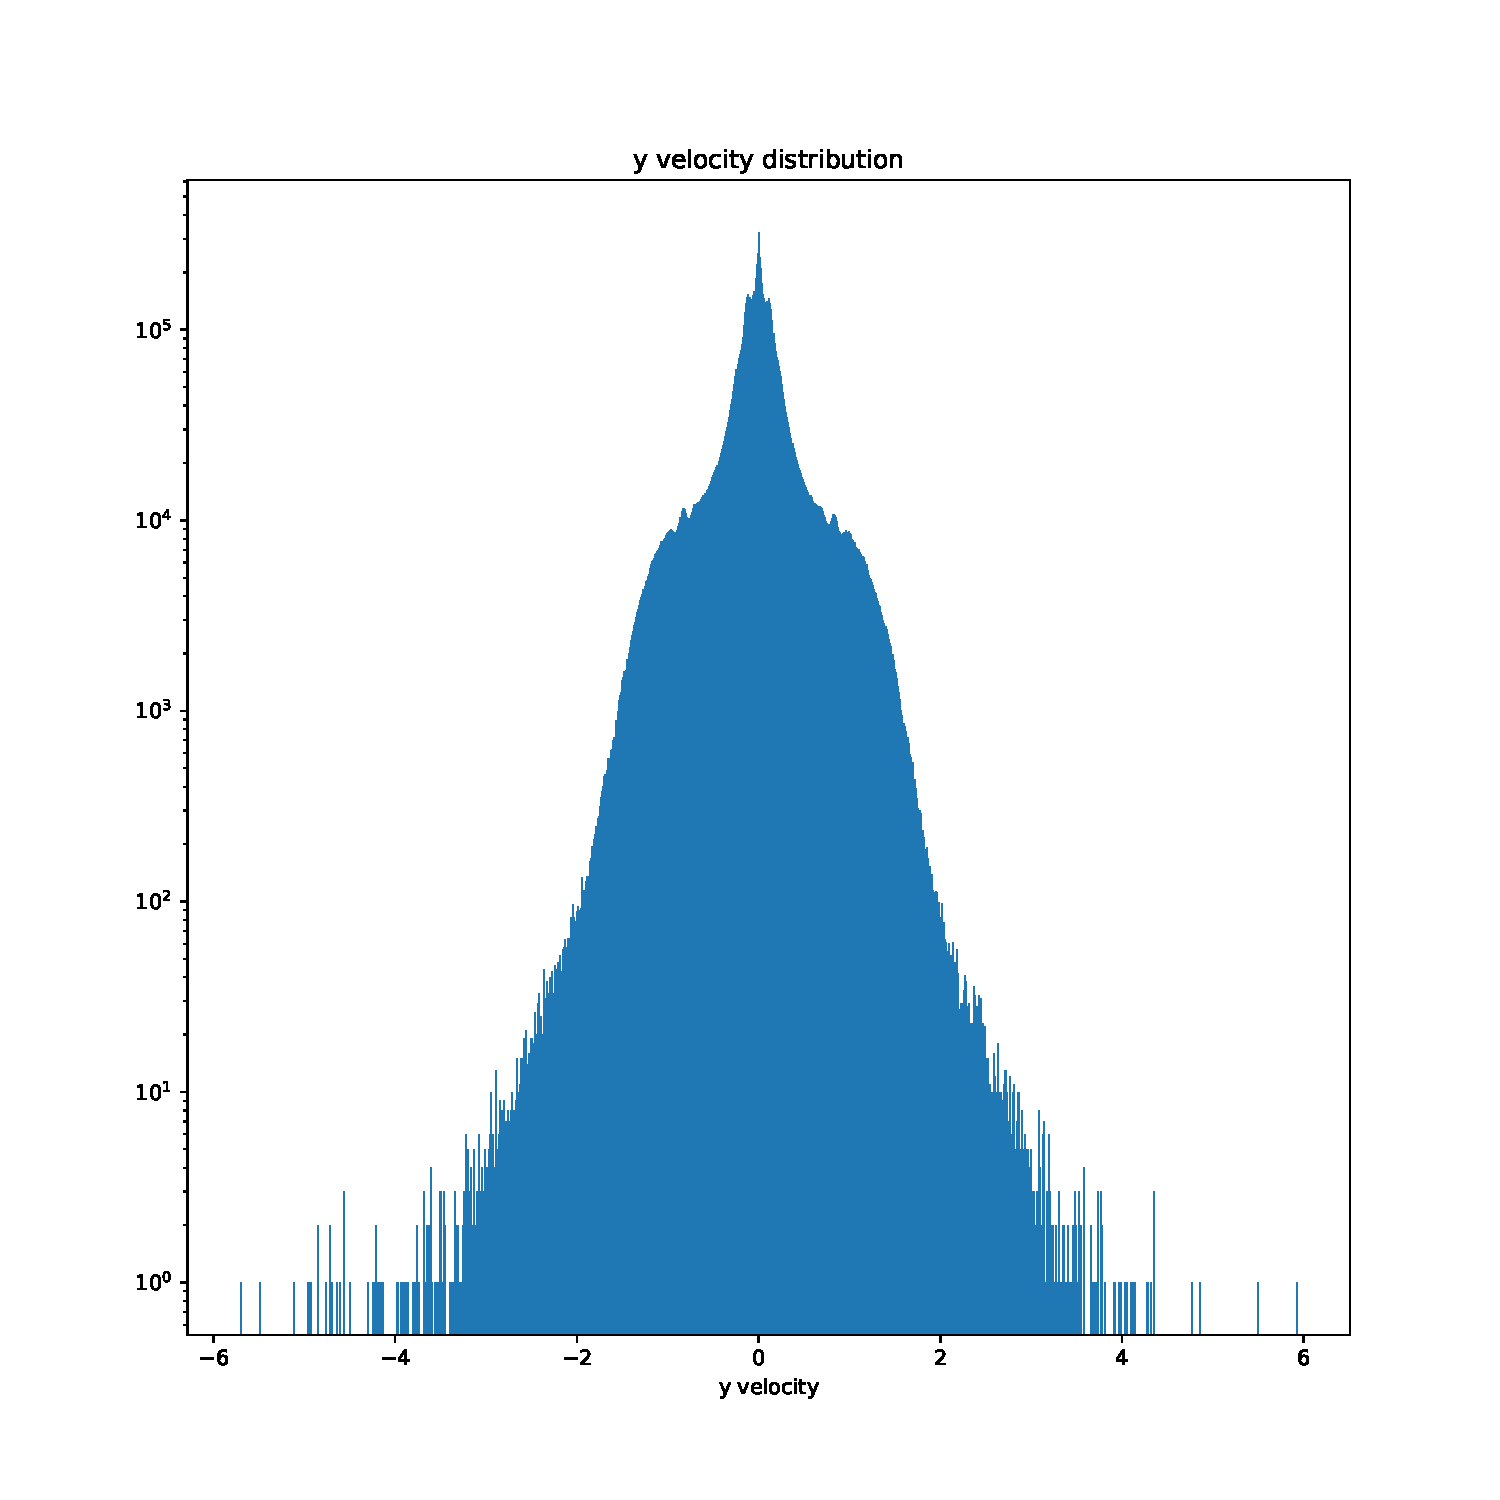
\includegraphics[ width=0.3\textwidth]{fig/hist_vy/save_trainf10_pro_RealData_hist_vy}
    }\quad\quad
    \subfloat[(ii) Simulation data hist vy]{
        \label{fig:Vy_SimD2Q9}
        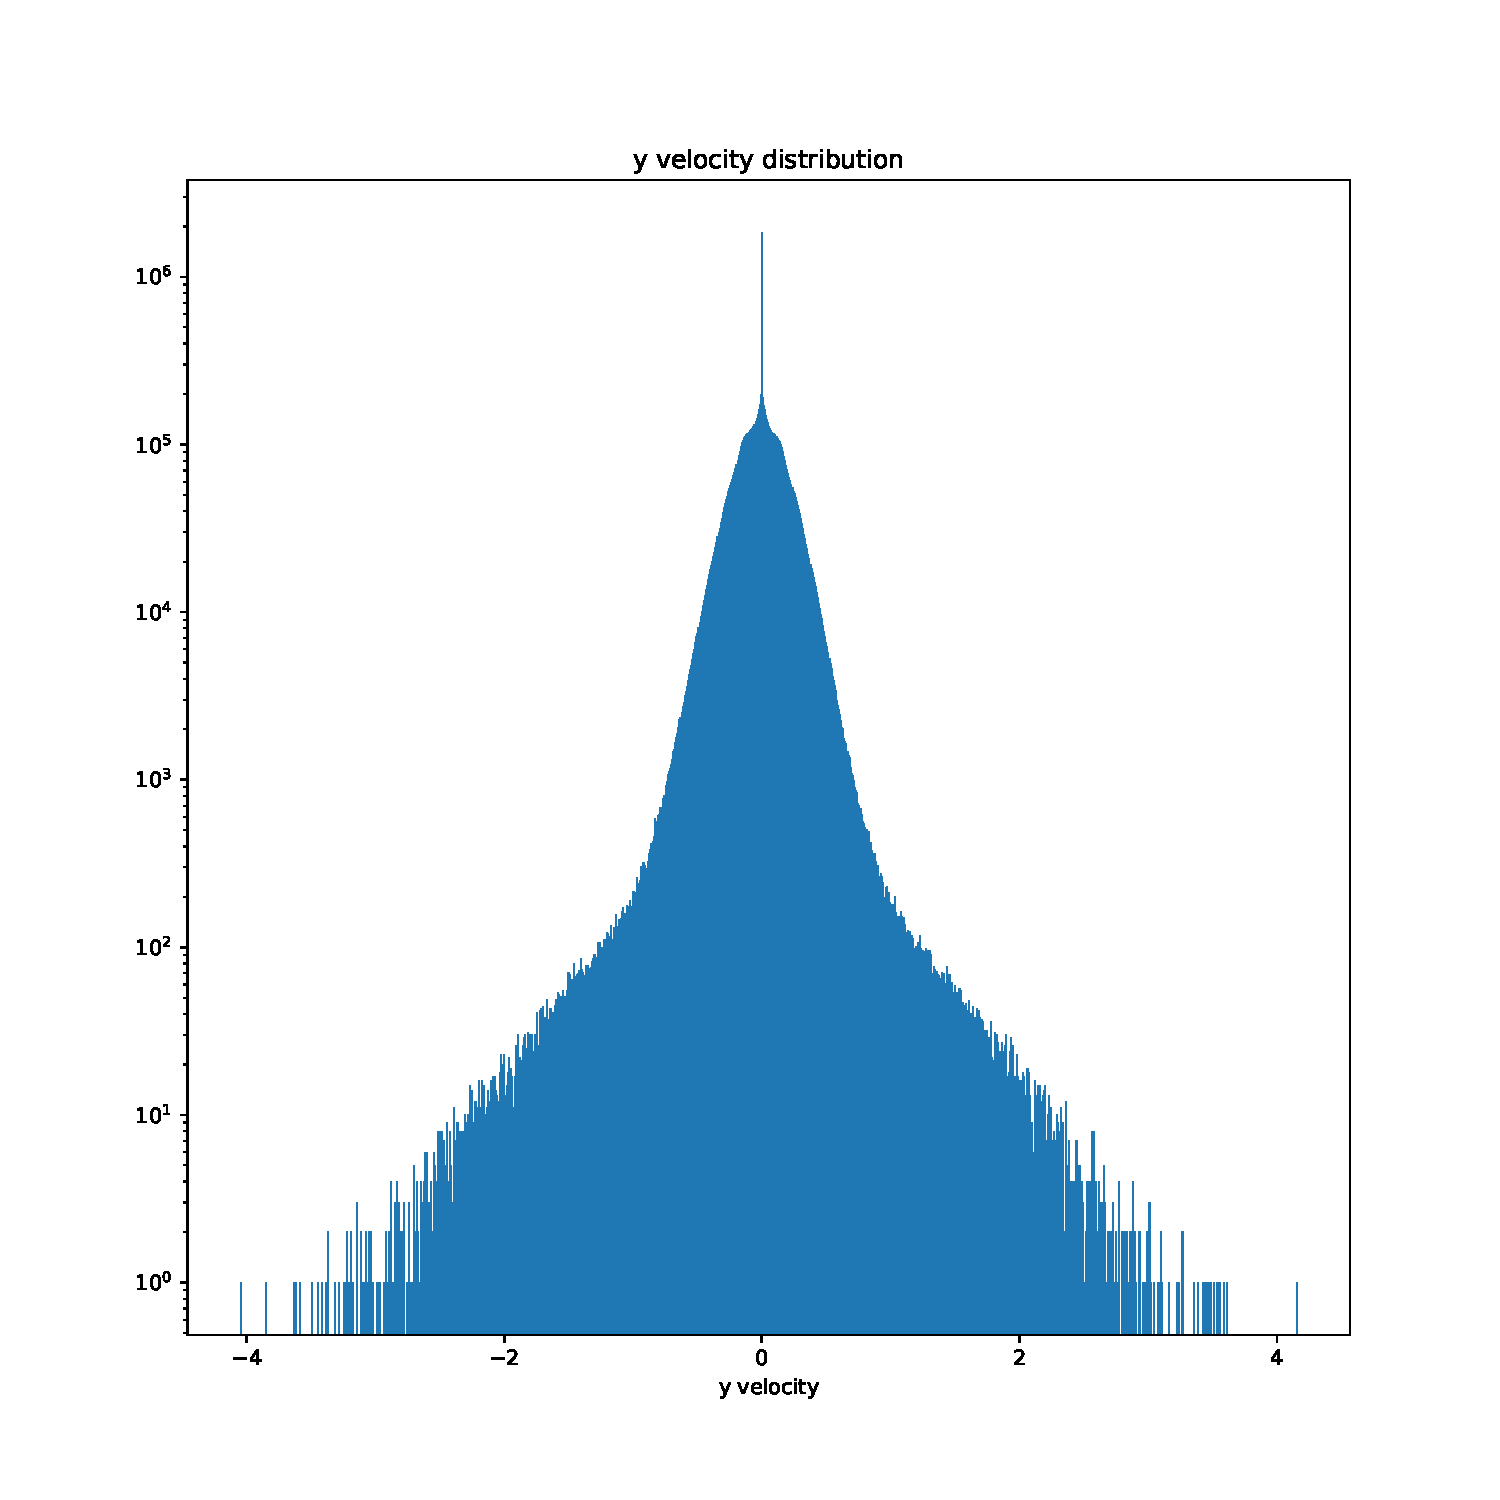
\includegraphics[ width=0.3\textwidth]{fig/hist_vy/save_trainf10_pro_simD2Q9_hist_vy}
    }
    \caption{(i) \& (ii) - simD2Q9 - The magnitude of the velocity vector along the $\vec x$ and $\vec y$ axis, plotted as 1-dimensional histograms.}
    \label{fig:hist_SimD2Q9}
\end{figure}
% --------------------------------------
\begin{figure}[!htb]
    \centering
        \subfloat[(iii) Real data hist2d xVx]{
        \label{fig:xVx_Real_iii}
        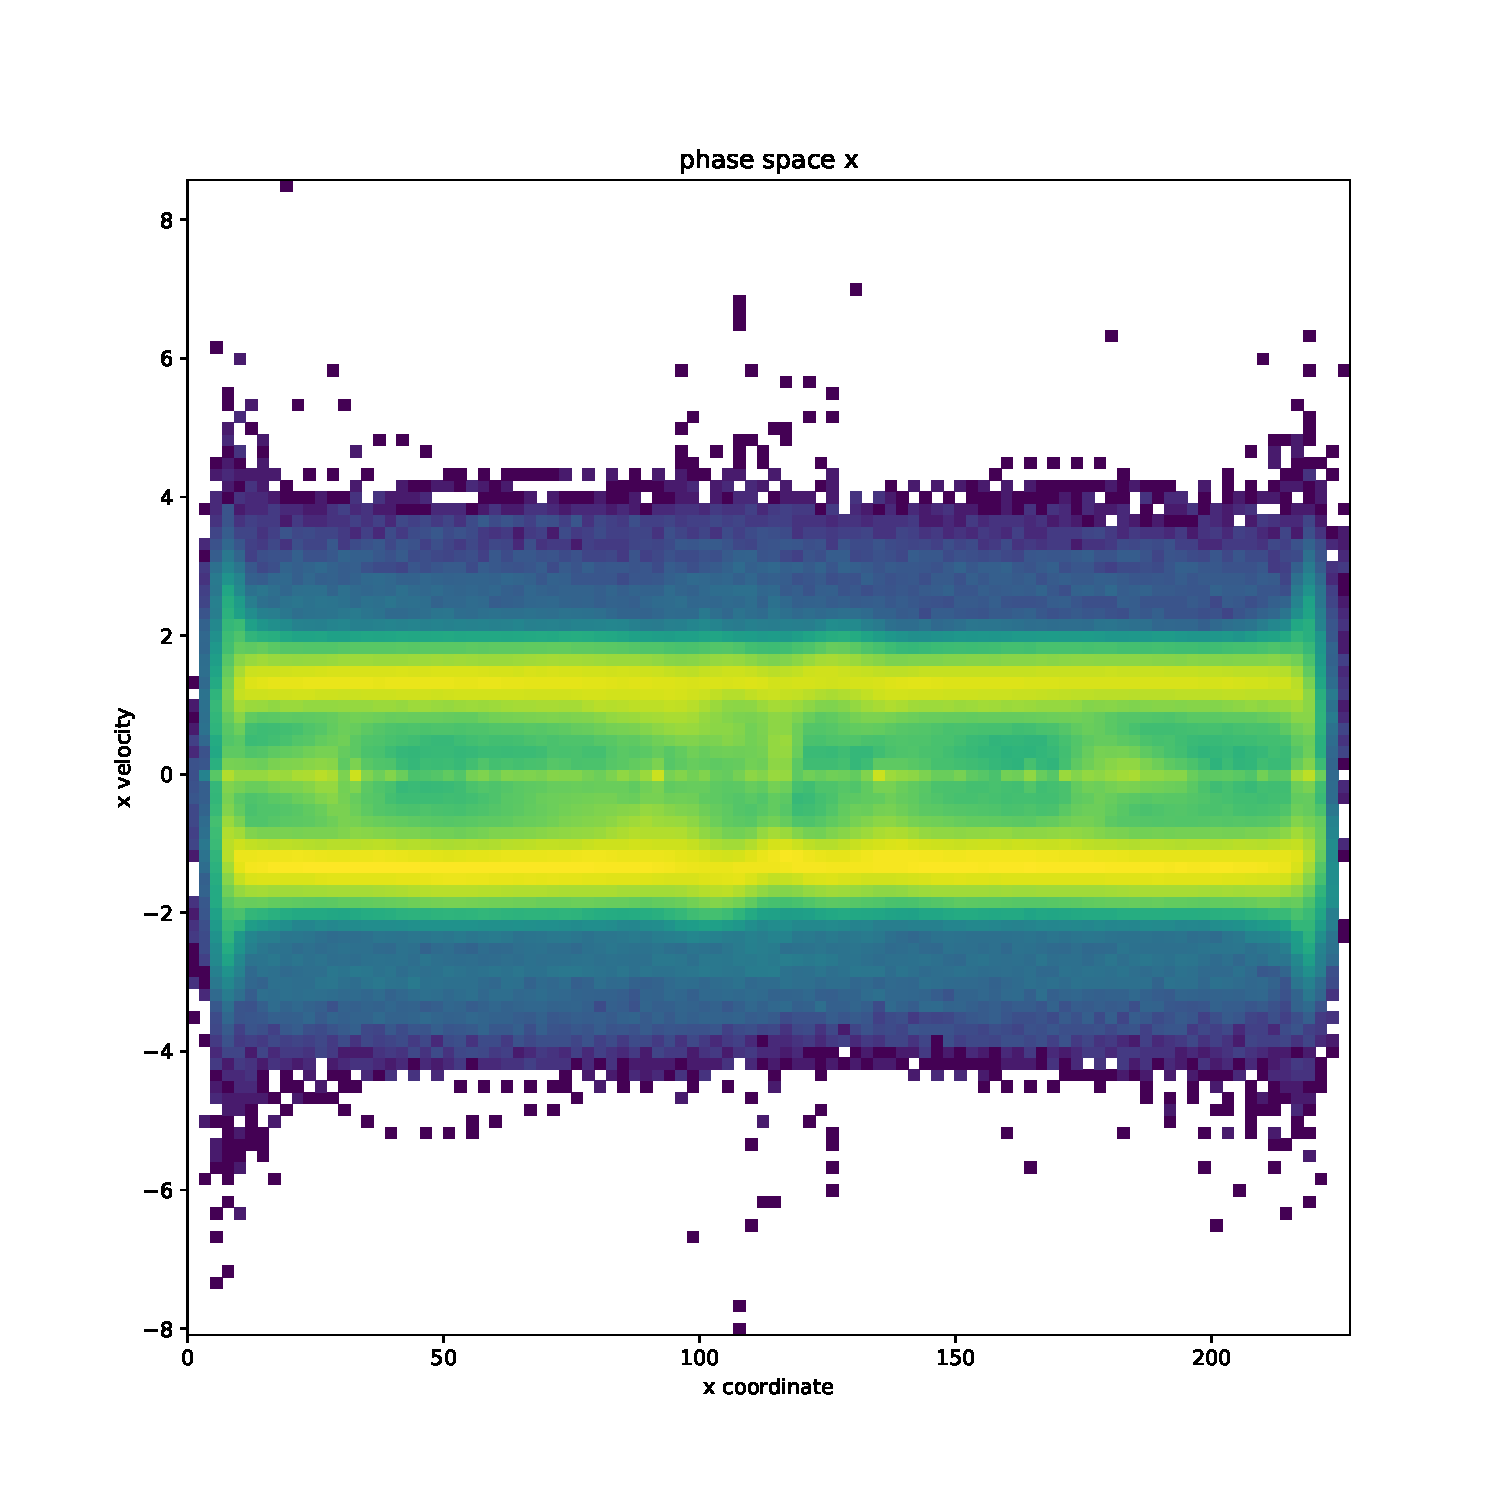
\includegraphics[ width=0.3\textwidth]{fig/hist2d_xvx/save_trainf10_pro_RealData_hist2d_x_vx}
    }\quad\quad
    \subfloat[(iii) Simulation data hist2d xVx]{
        \label{fig:xVx_SimD2Q9}
        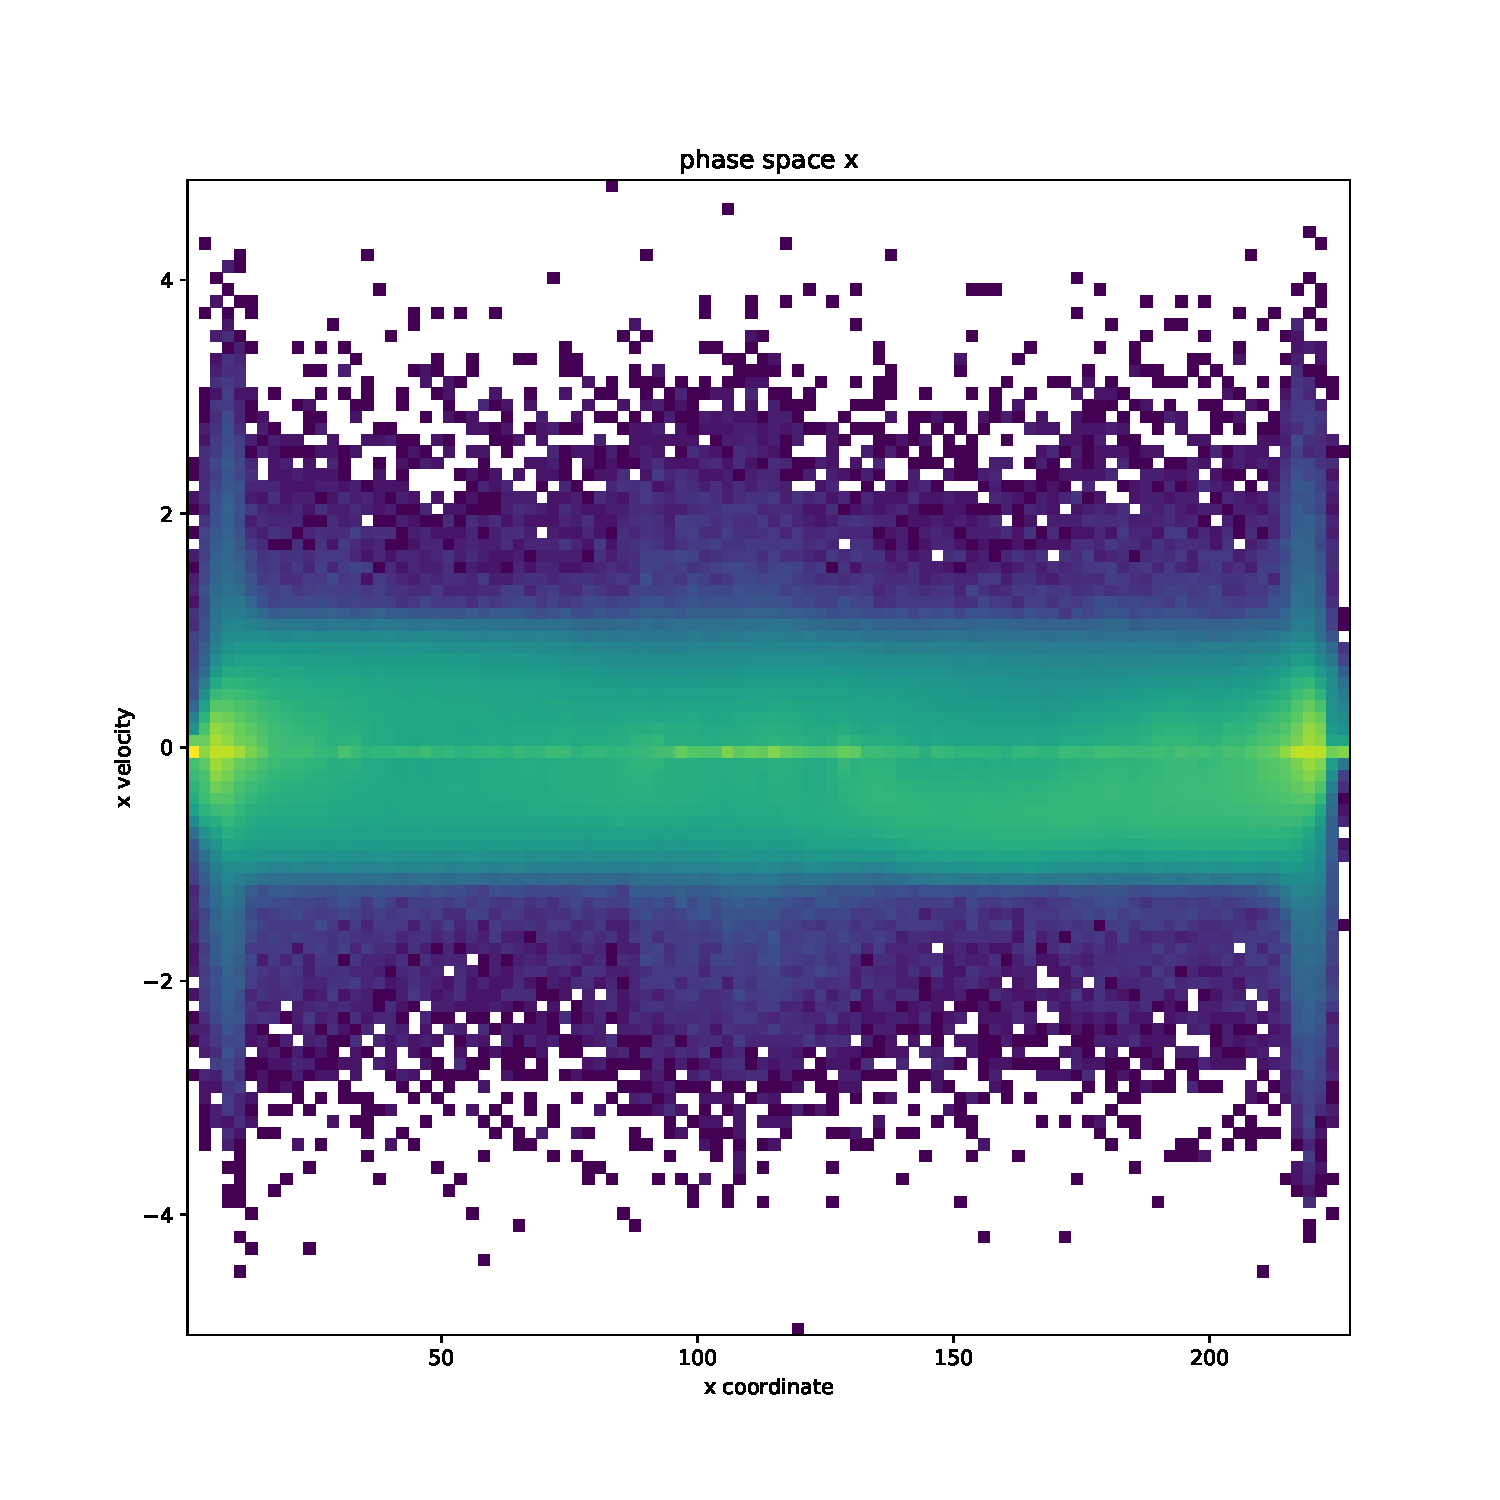
\includegraphics[ width=0.3\textwidth]{fig/hist2d_xvx/save_trainf10_pro_simD2Q9_hist2d_x_vx}
    }\quad\quad
    \subfloat[(iv) Real data hist2d yVy]{
        \label{fig:yvy_Real_iv}
        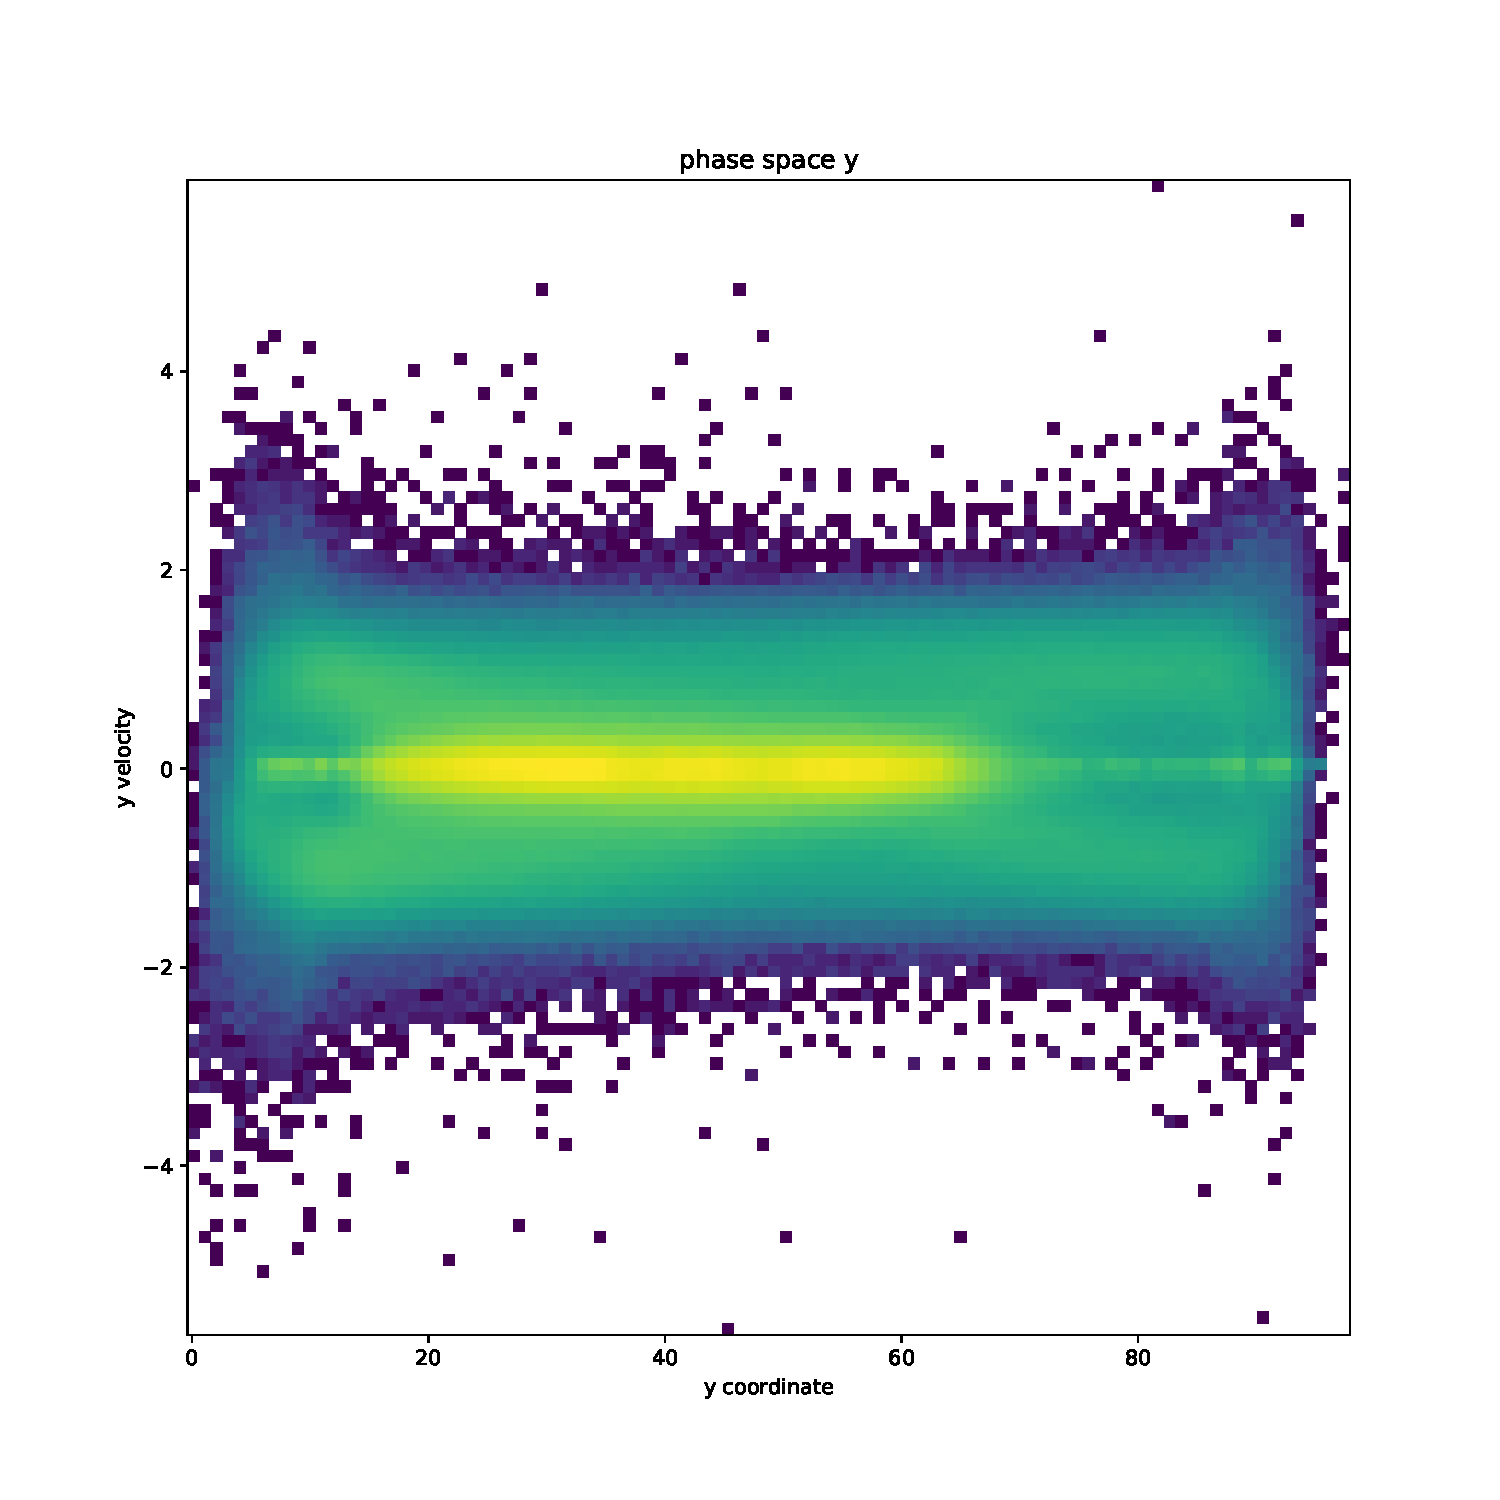
\includegraphics[ width=0.3\textwidth]{fig/hist2d_yvy/save_trainf10_pro_RealData_hist2d_y_vy}
    }\quad\quad
    \subfloat[(iv) Simulation data hist2d yVy]{
        \label{fig:yVy_SimD2Q9}
        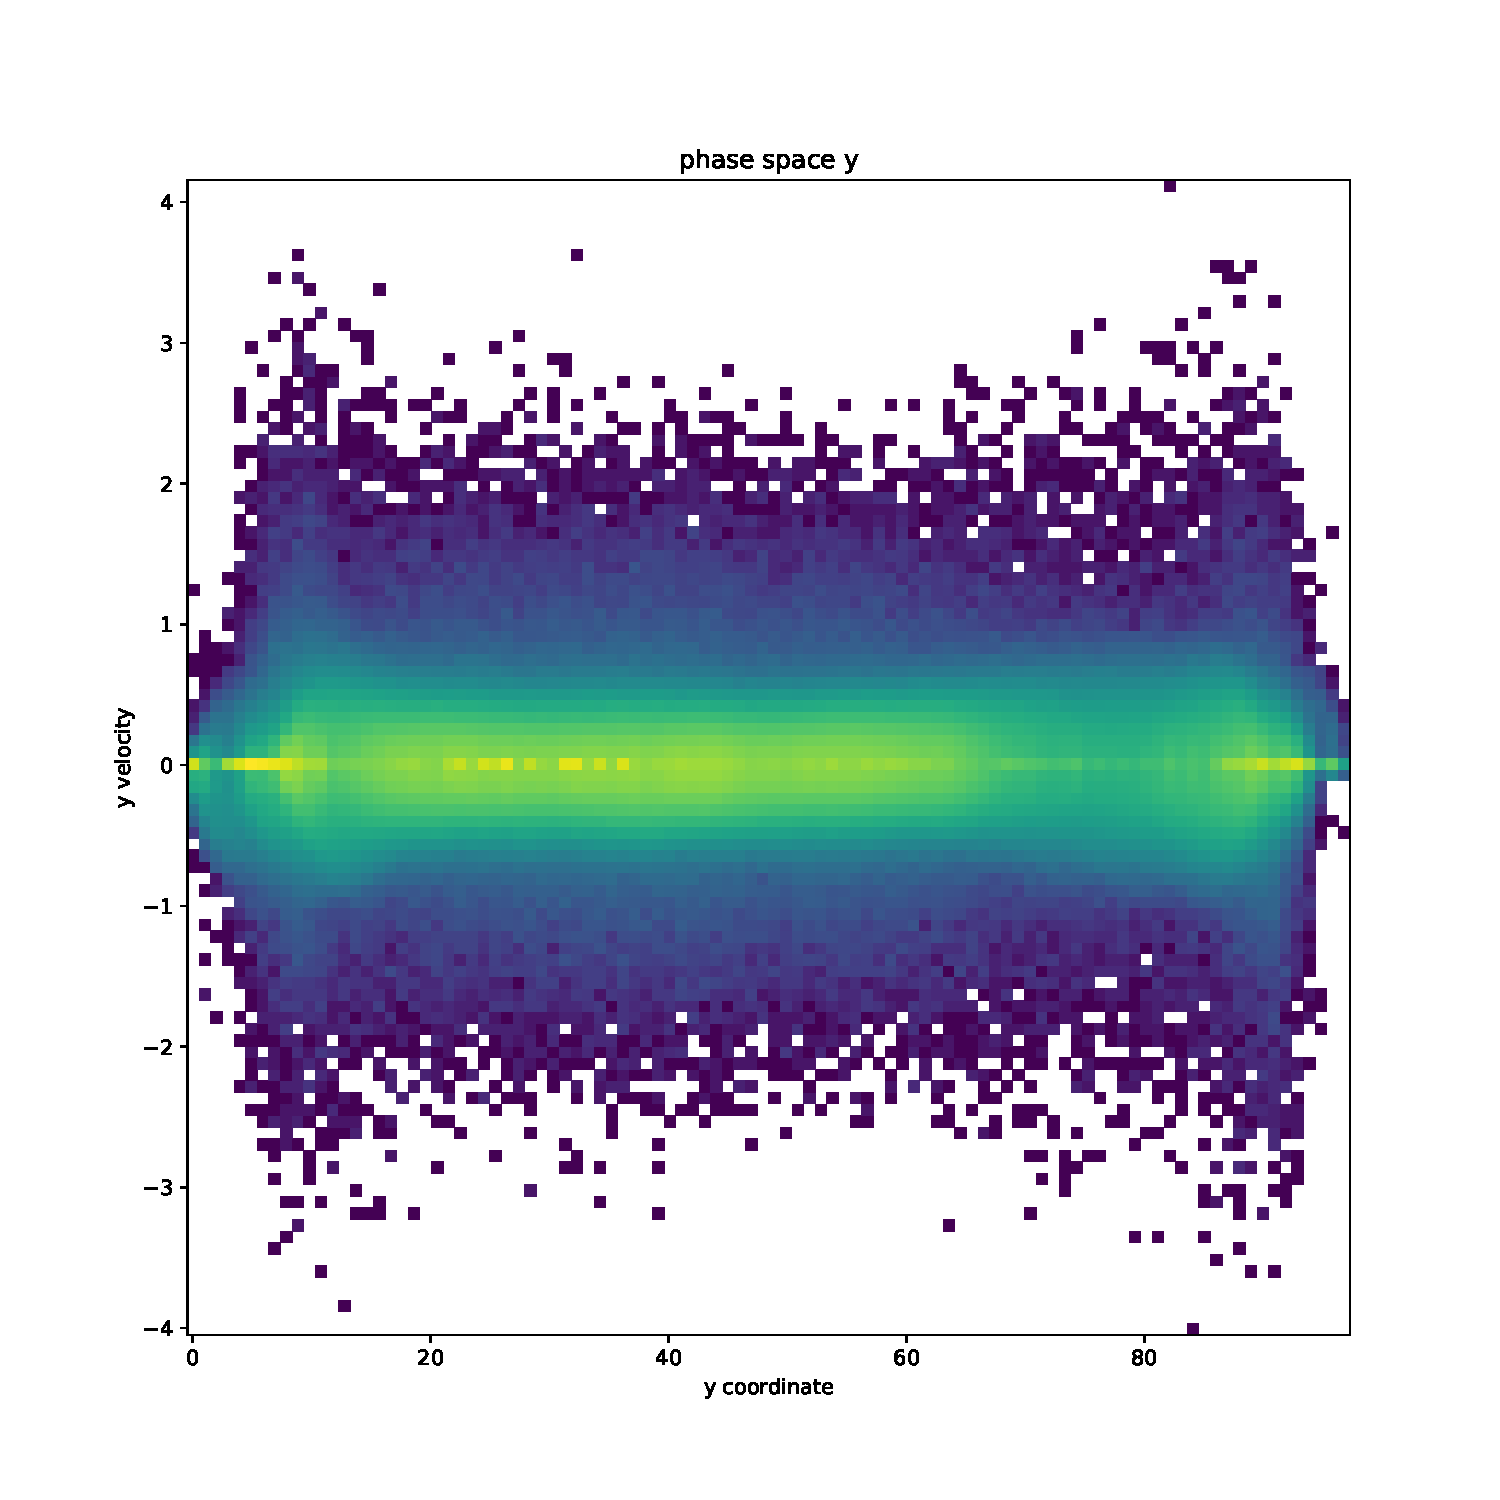
\includegraphics[ width=0.3\textwidth]{fig/hist2d_yvy/save_trainf10_pro_simD2Q9_hist2d_y_vy}
    }
    \caption{(iii) \& (iv) - simD2Q9 - The correlation between the position along the $\vec x$ and $\vec y$ axis and the magnitude of the velocity vector along the same correspondent axes, plotted as heat-map or 2-dimensional histograms.}
    \label{fig:hist2d_SimD2Q9}
\end{figure}
% --------------------------------------
\begin{figure}[!htb]
    \centering
        \subfloat[(v) Real data hist2d Pxy]{
        \label{fig:Pxy_Real_v}
        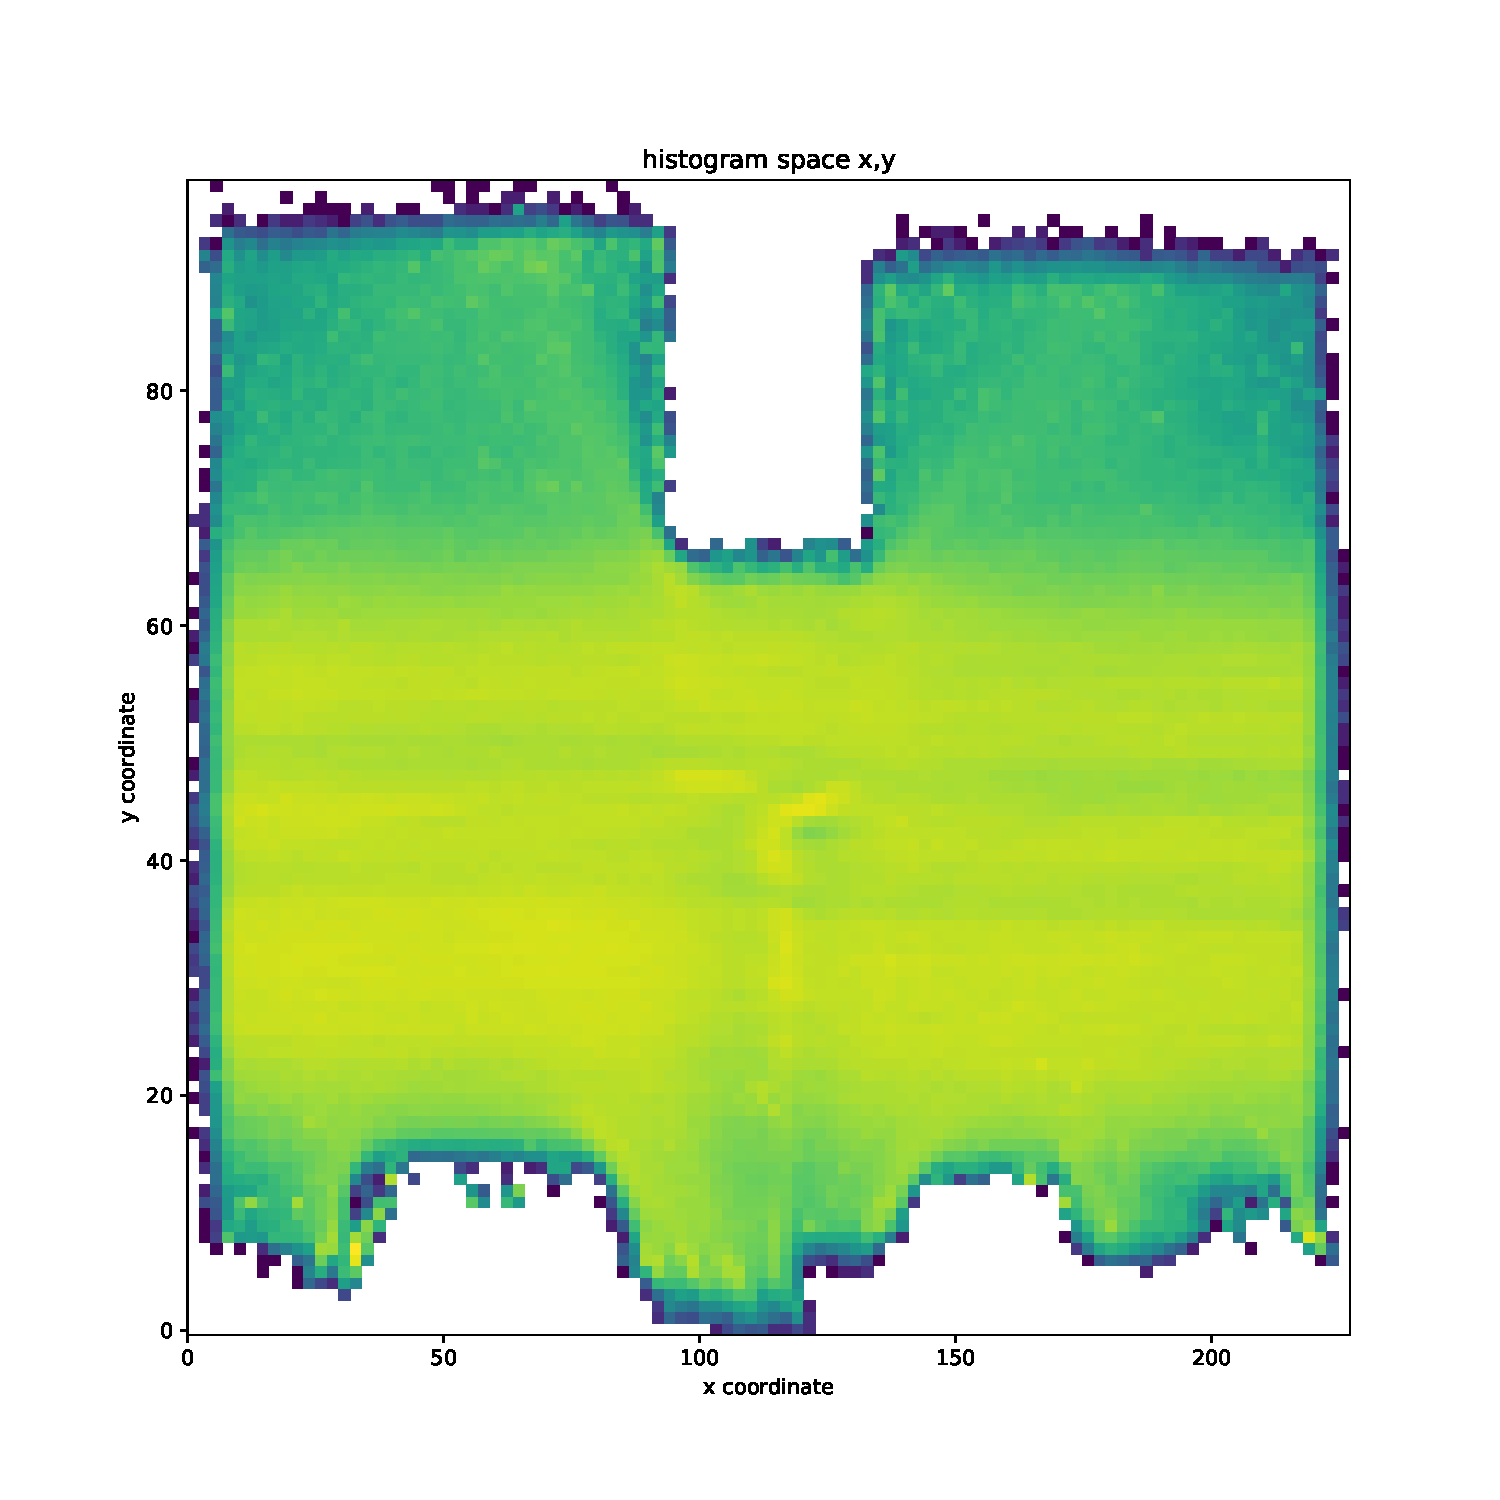
\includegraphics[ width=0.3\textwidth]{fig/hist2d_pxy/save_trainf10_pro_RealData_hist2d_x_y}
    }\quad\quad
    \subfloat[(v) Simulation data hist2d Pxy]{
        \label{fig:Pxy_SimD2Q9}
        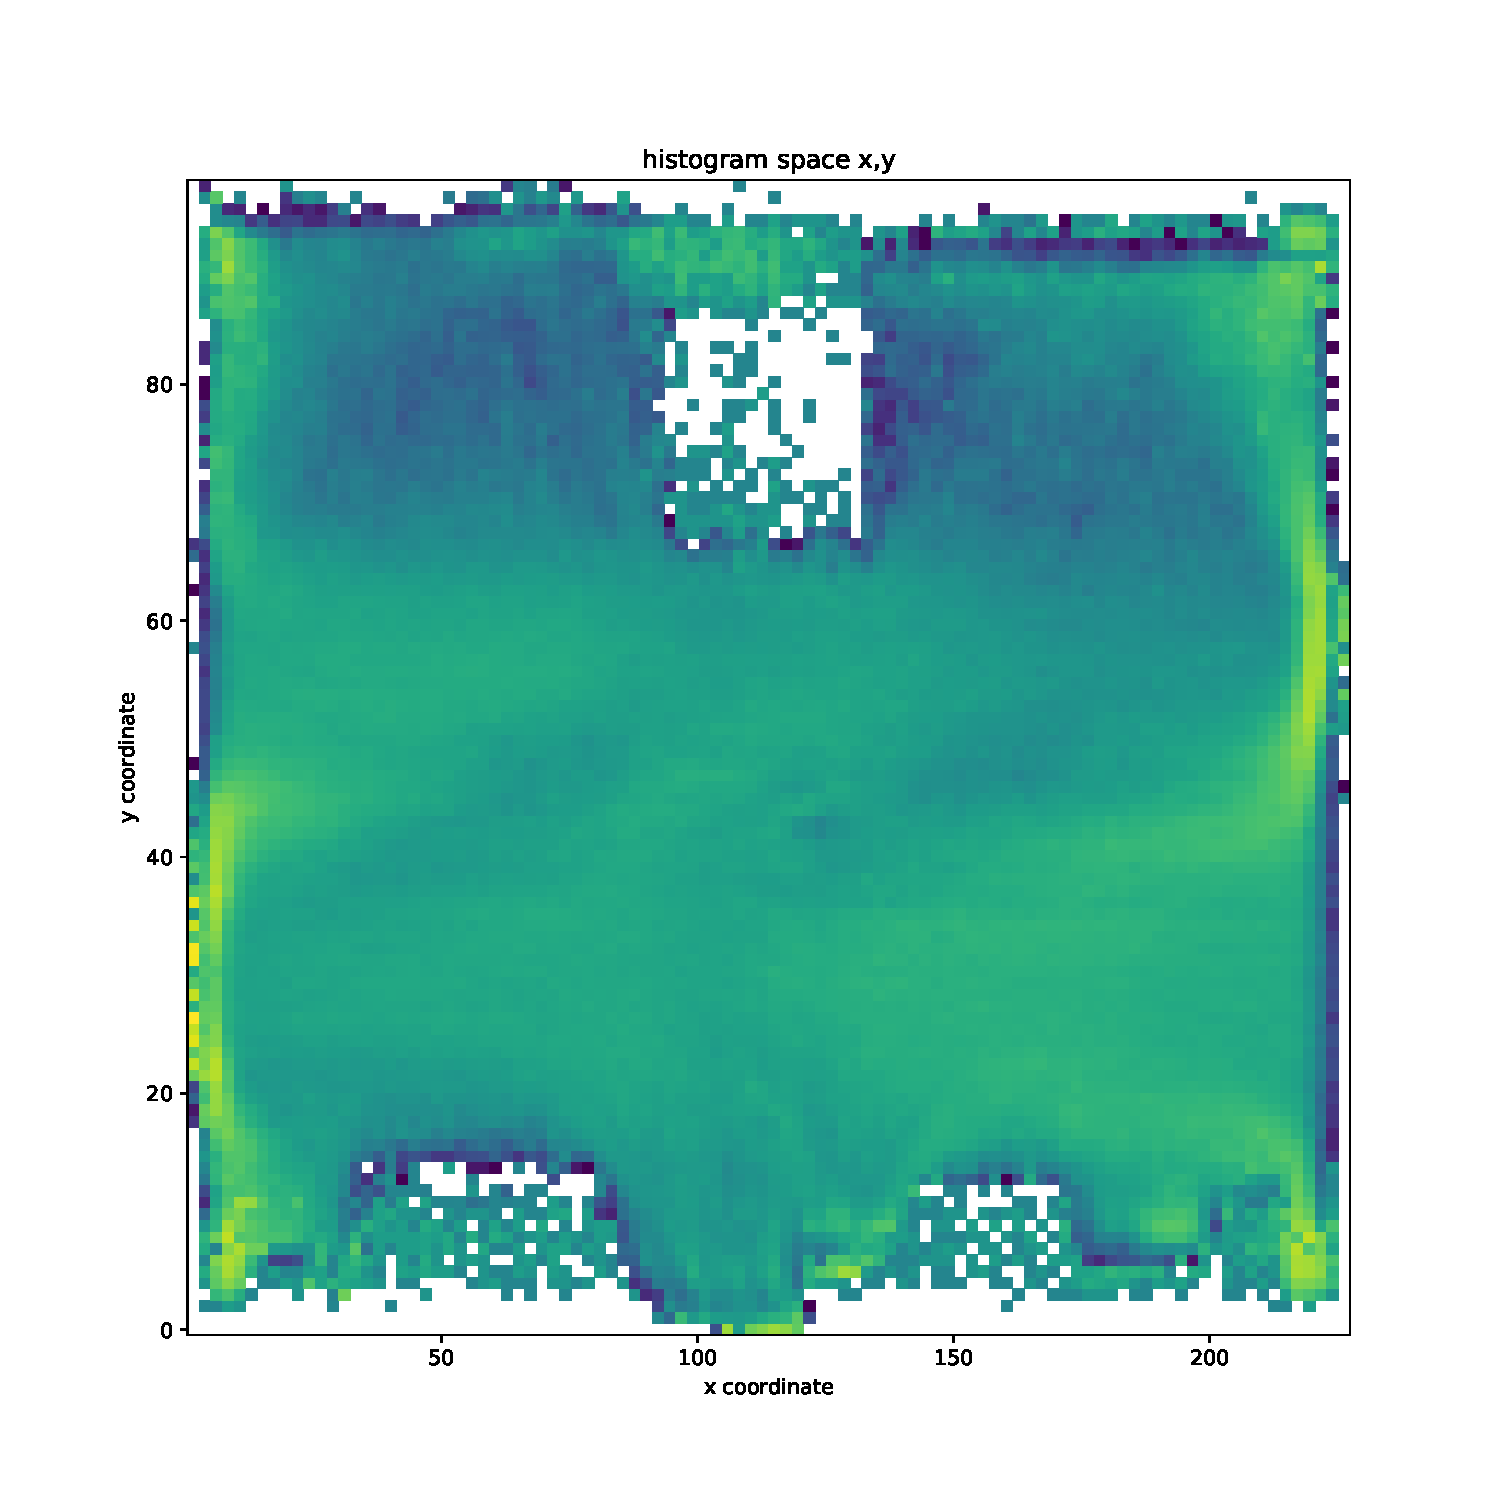
\includegraphics[ width=0.3\textwidth]{fig/hist2d_pxy/save_trainf10_pro_simD2Q9_hist2d_x_y}
    }
    \caption{(v) - simD2Q9 - The heat-map of the positions along $\vec x$ and $\vec y$ axis of all paths that have passed though, plotted as 2-dimensional histogram.}
    \label{fig:Pxy_SimD2Q9}
\end{figure}


\FloatBarrier
% -------------------------------------------------------------------------------------------------------------------------------------------------------------------------------------------
\subsection{Real data - D2Q9Q9}
This paragraph's reference are the following: (Figure \ref{fig:hist_SimD2Q9Q9}), (Figure \ref{fig:hist2d_SimD2Q9Q9}), (Figure \ref{fig:Pxy_SimD2Q9Q9}) 

\begin{figure}[!htb]
    \centering
    \subfloat[(i) Real data hist vx]{
        \label{fig:Vx_Real_i}
        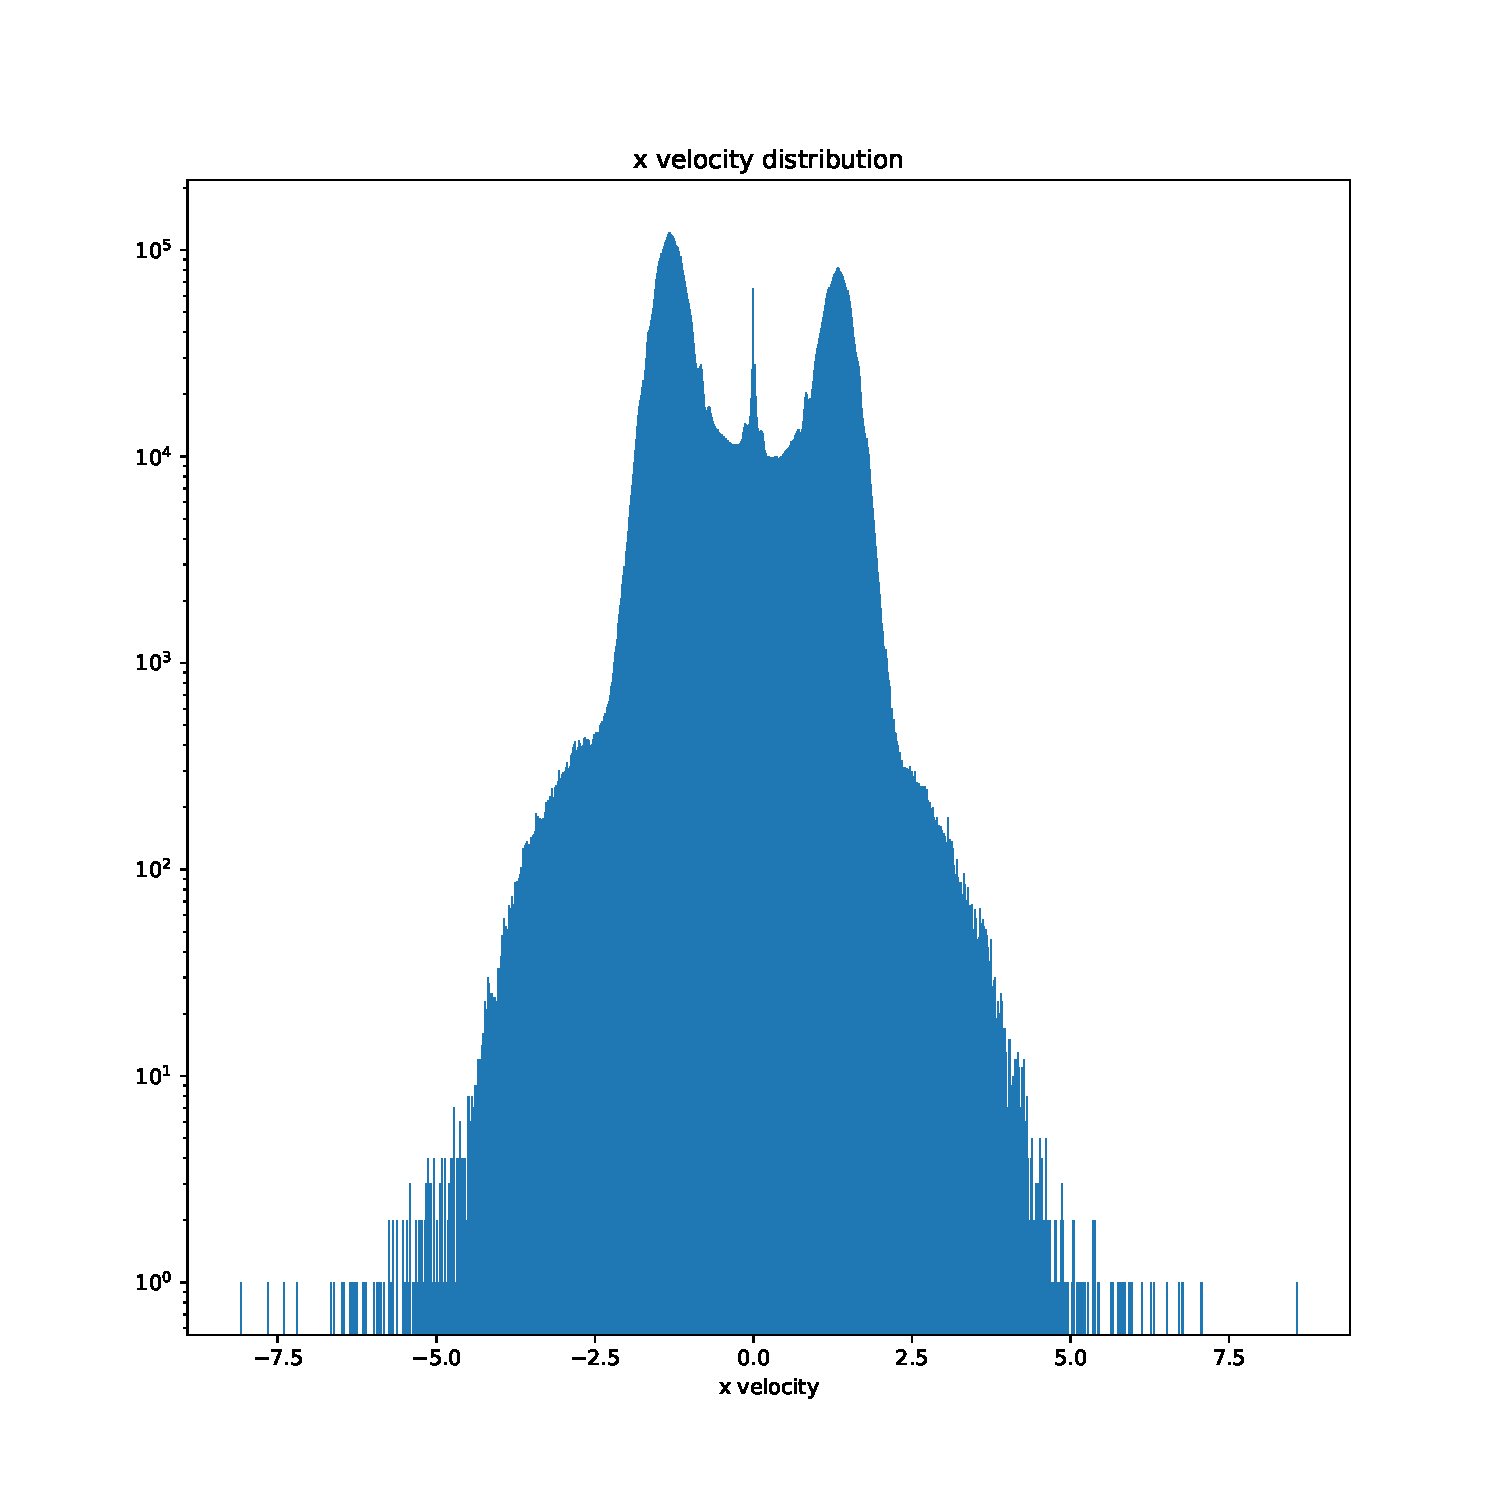
\includegraphics[ width=0.3\textwidth]{fig/hist_vx/save_trainf10_pro_RealData_hist_vx}
    }\quad\quad
    \subfloat[(i) Simulation data hist vx]{
        \label{fig:Vx_SimD2Q9Q9}
        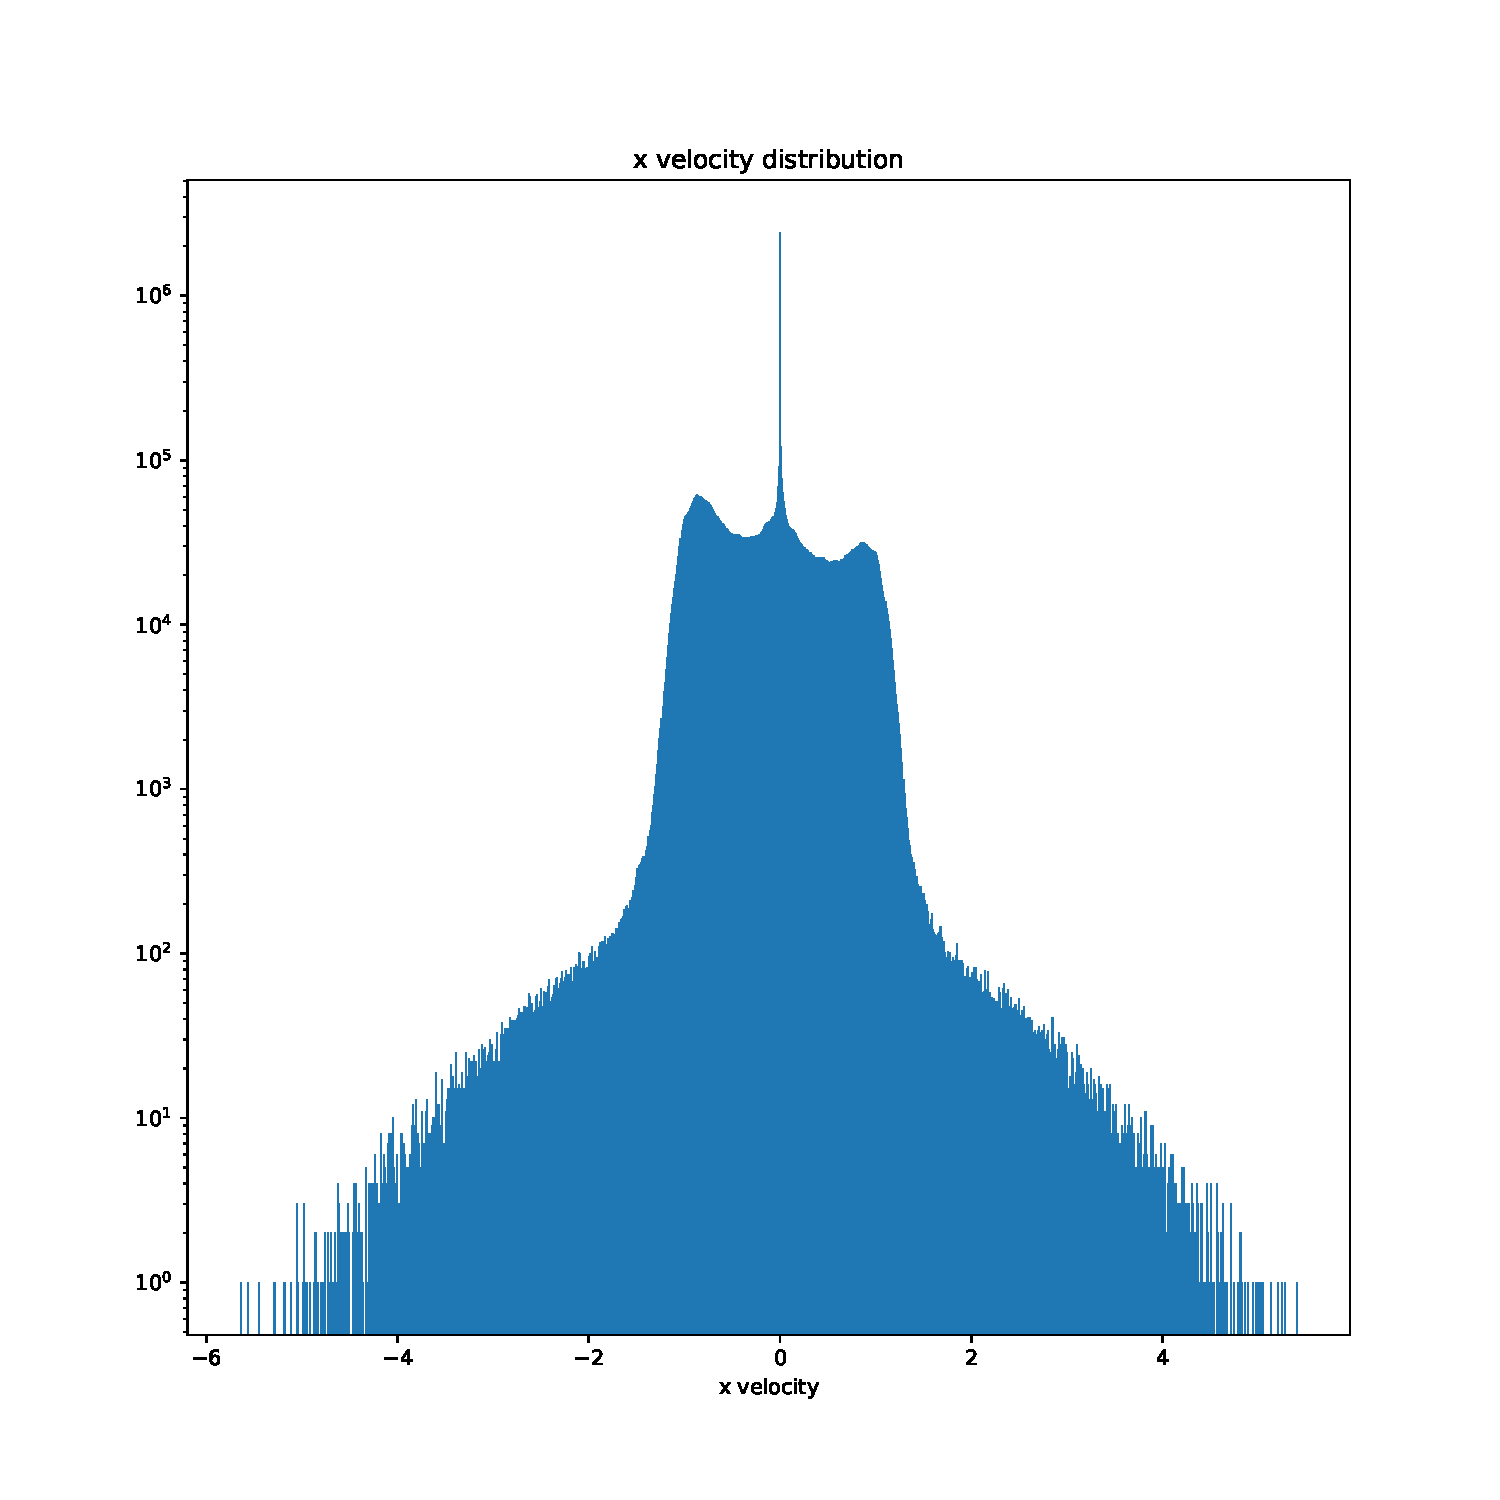
\includegraphics[ width=0.3\textwidth]{fig/hist_vx/save_trainf10_pro_simD2Q9Q9_hist_vx}
    }\quad\quad
    \subfloat[(ii) Real data hist vy]{
        \label{fig:Vy_Real_ii}
        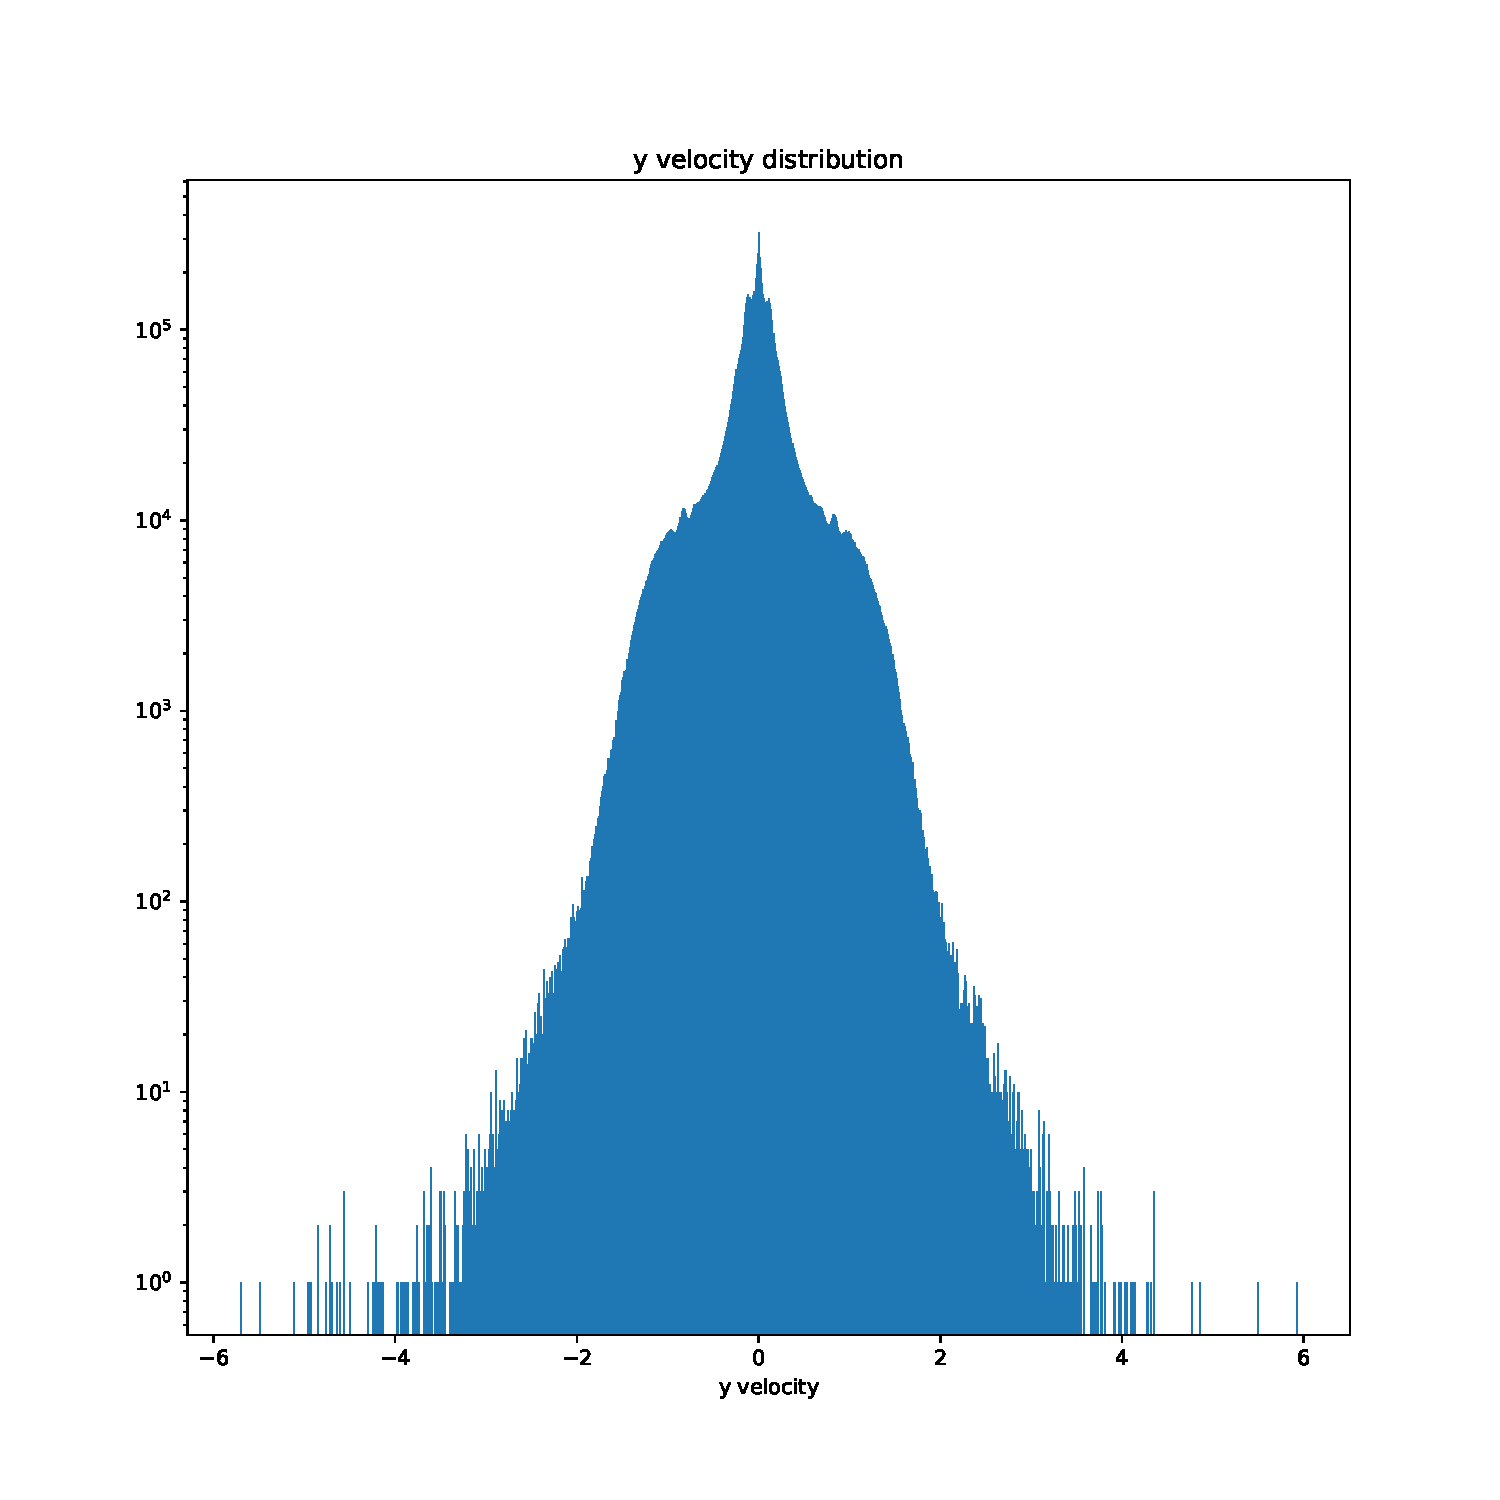
\includegraphics[ width=0.3\textwidth]{fig/hist_vy/save_trainf10_pro_RealData_hist_vy}
    }\quad\quad
    \subfloat[(ii) Simulation data hist vy]{
        \label{fig:Vy_SimD2Q9Q9}
        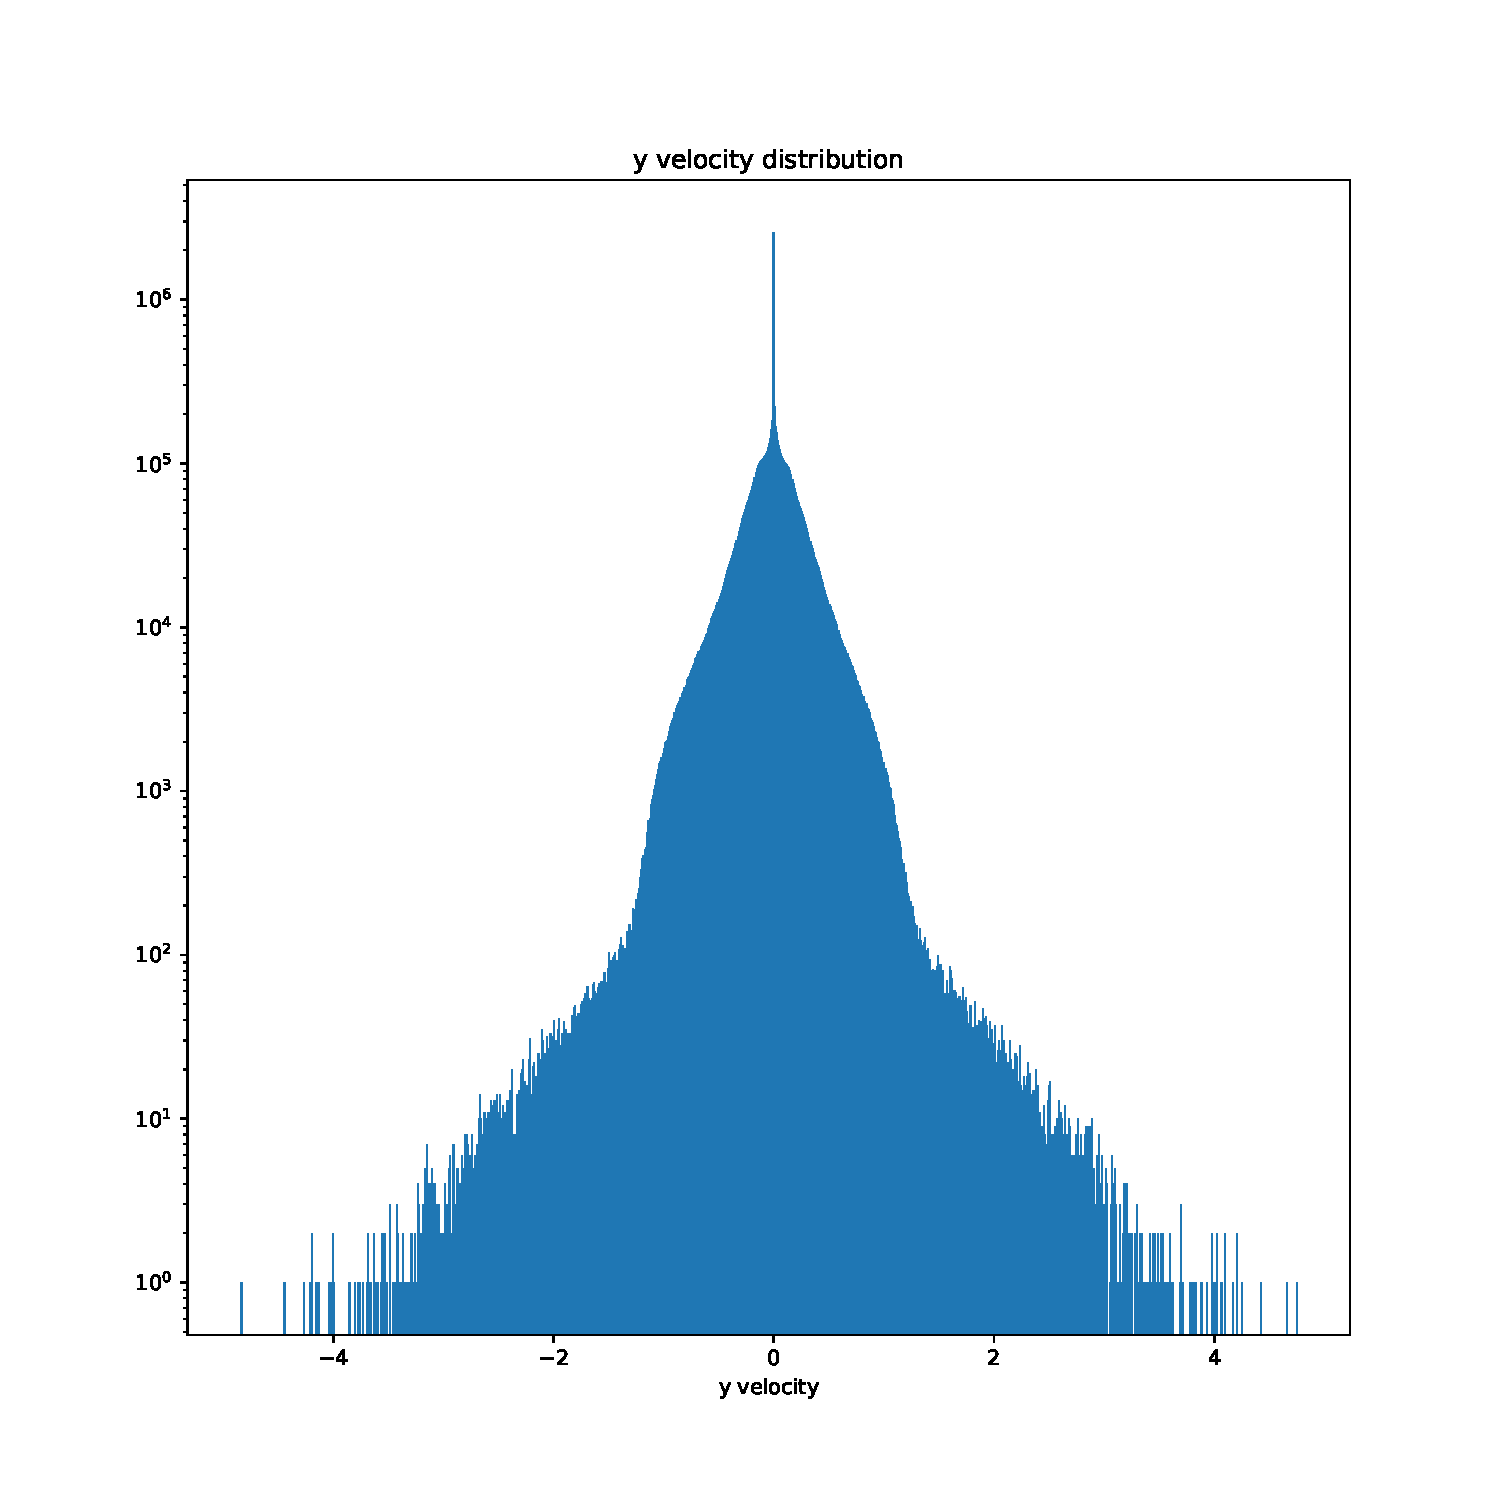
\includegraphics[ width=0.3\textwidth]{fig/hist_vy/save_trainf10_pro_simD2Q9Q9_hist_vy}
    }
    \caption{(i) \& (ii) - simD2Q9Q9 - The magnitude of the velocity vector along the $\vec x$ and $\vec y$ axis, plotted as 1-dimensional histograms.}
    \label{fig:hist_SimD2Q9Q9}
\end{figure}
% --------------------------------------
\begin{figure}[!htb]
    \centering
        \subfloat[(iii) Real data hist2d xVx]{
        \label{fig:xVx_Real_iii}
        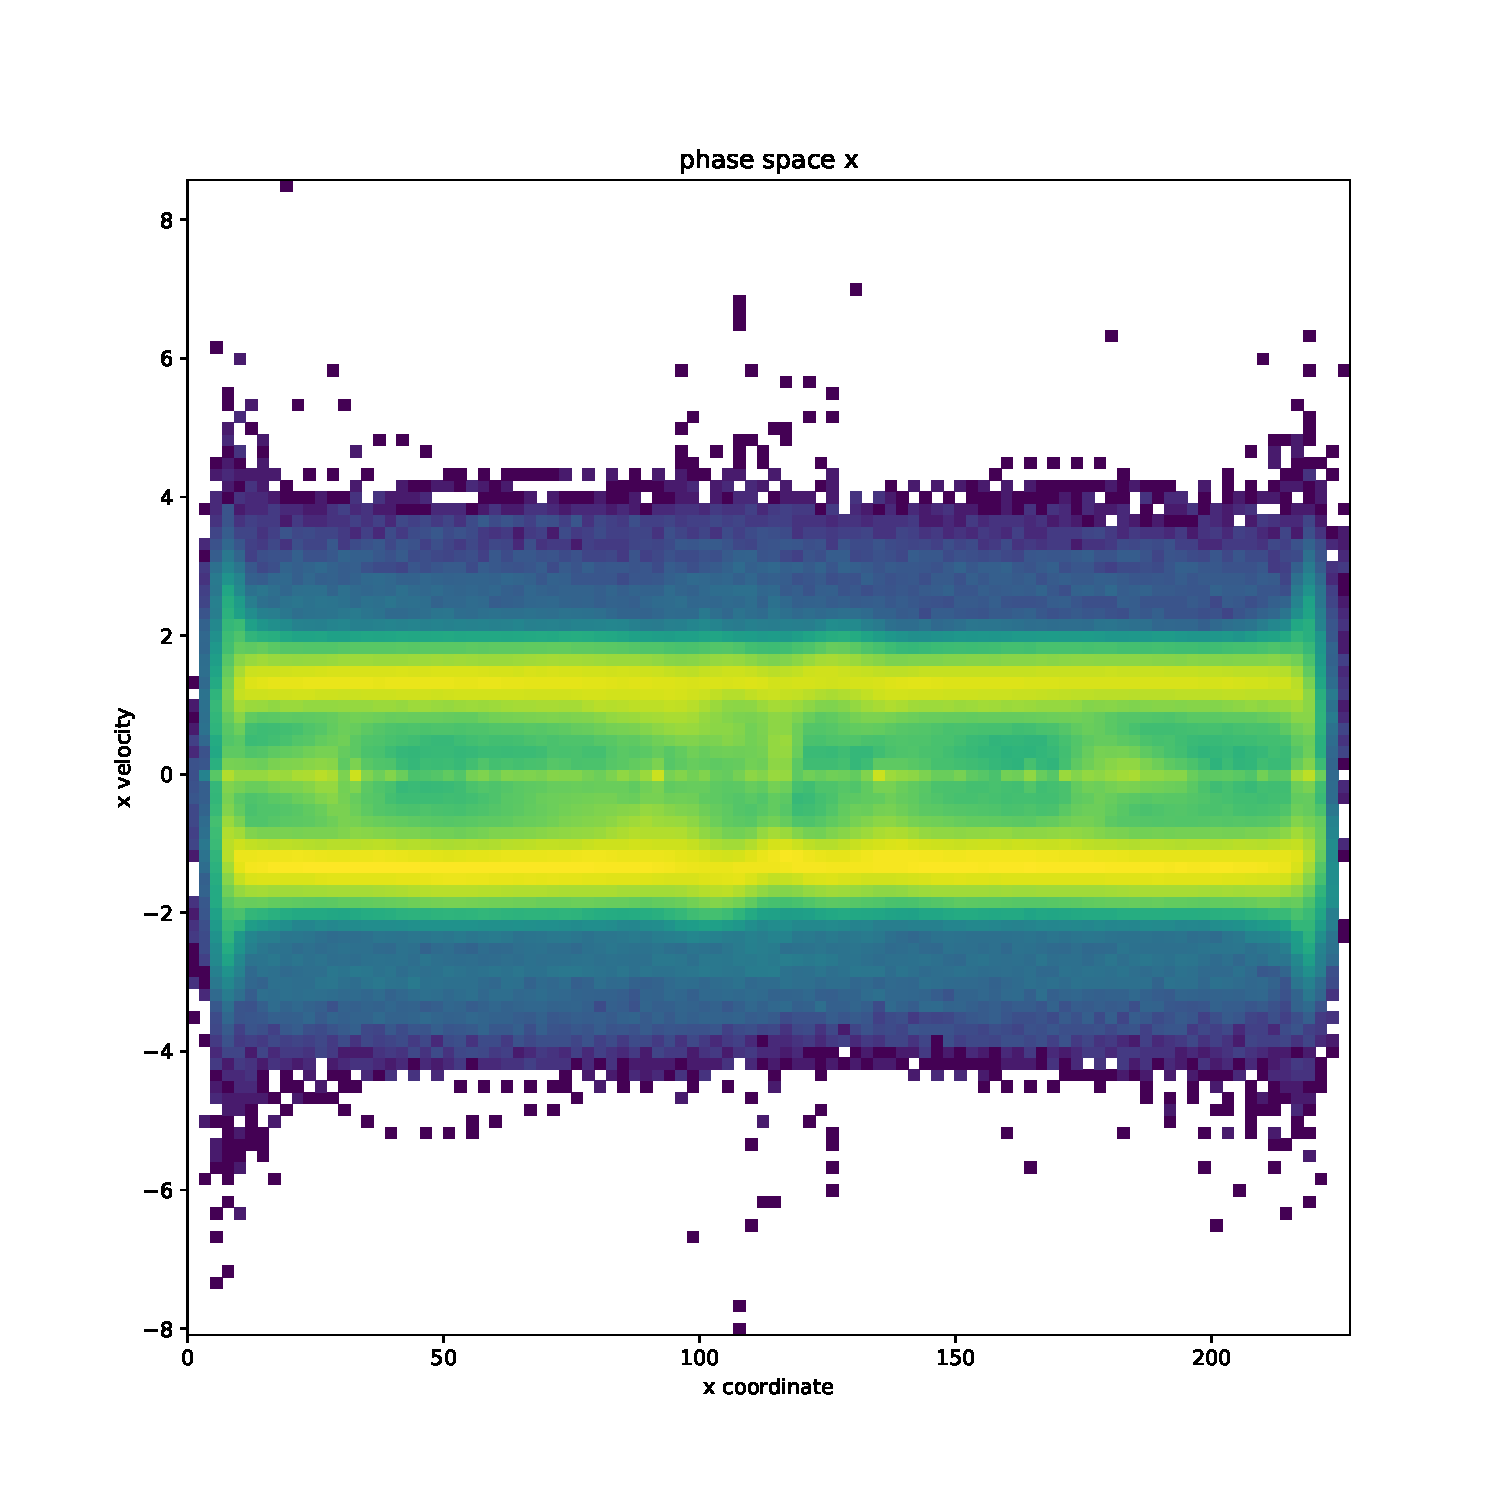
\includegraphics[ width=0.3\textwidth]{fig/hist2d_xvx/save_trainf10_pro_RealData_hist2d_x_vx}
    }\quad\quad
    \subfloat[(iii) Simulation data hist2d xVx]{
        \label{fig:xVx_SimD2Q9Q9}
        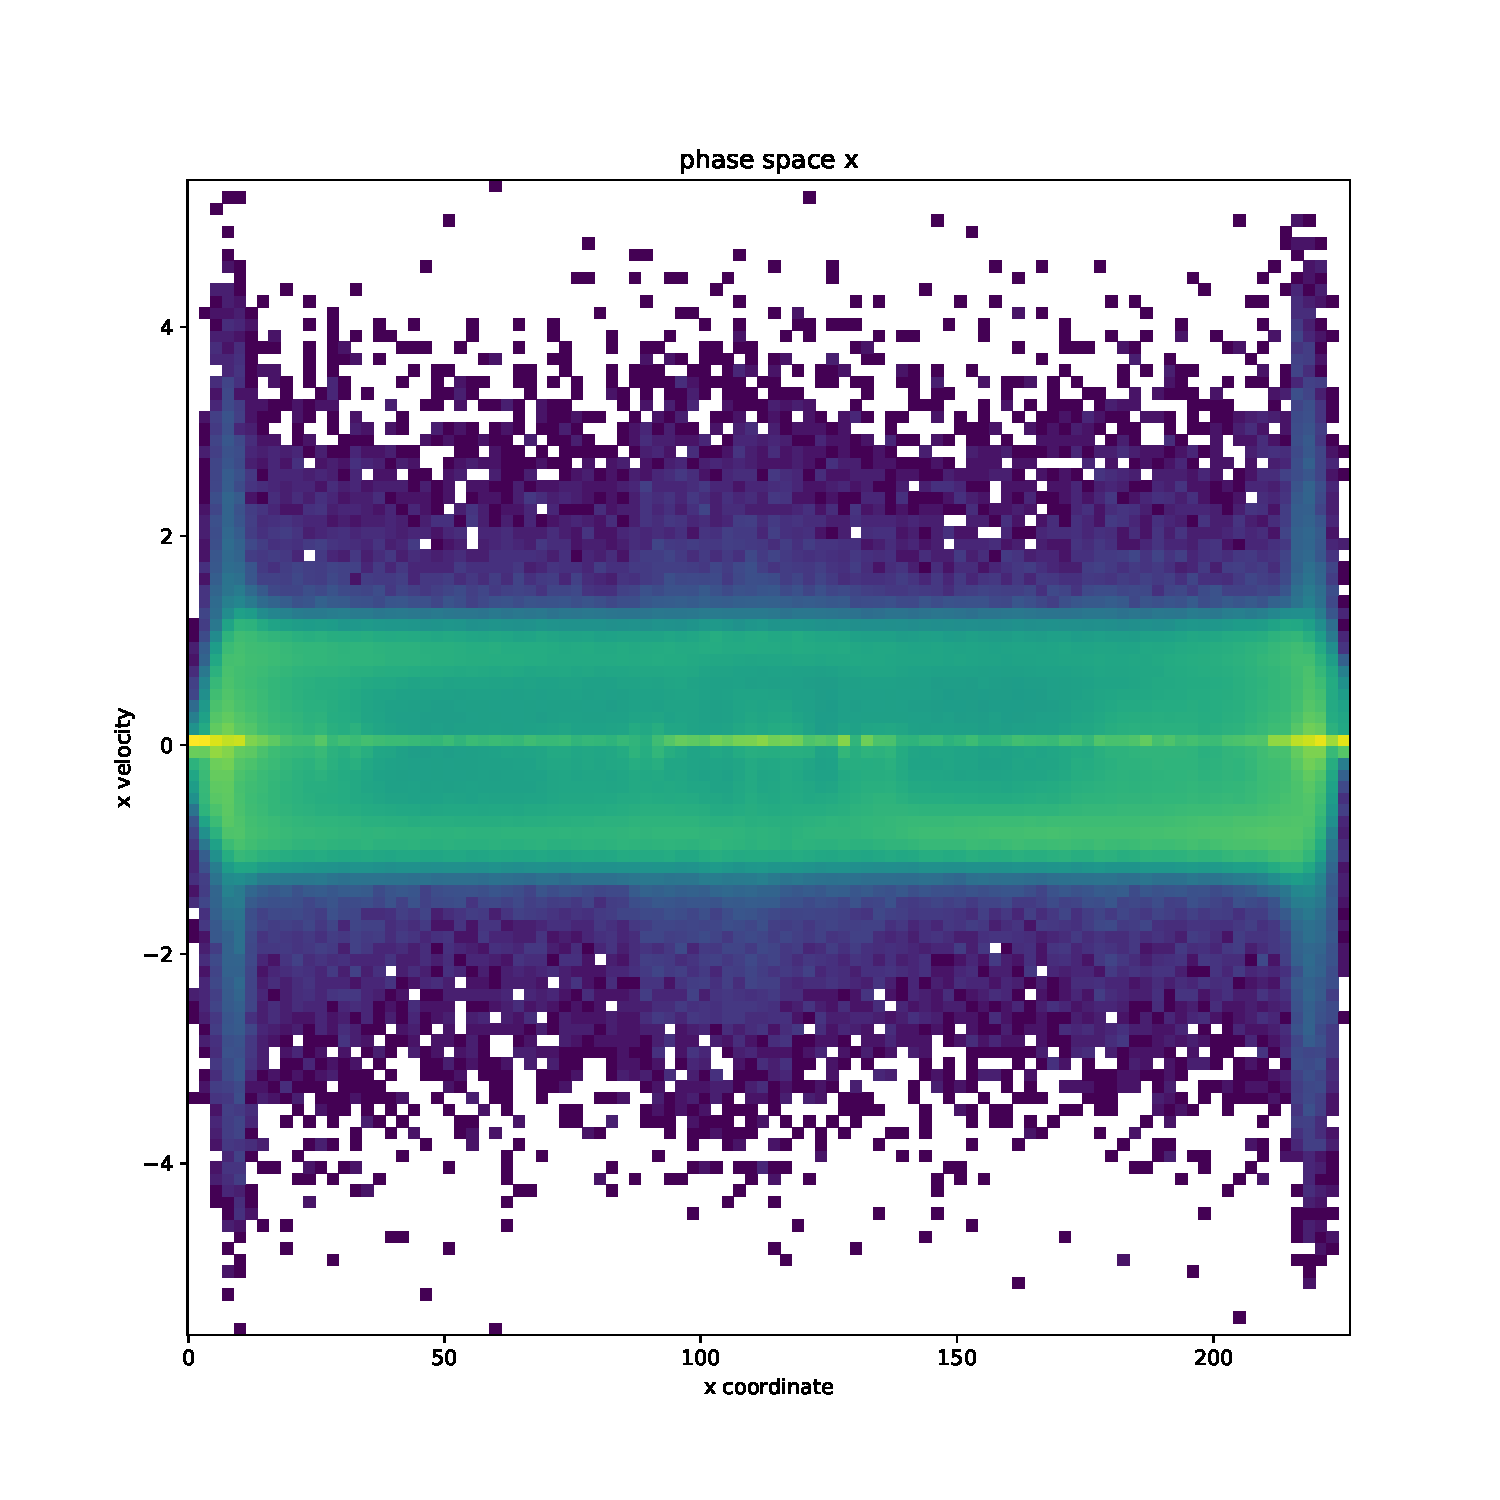
\includegraphics[ width=0.3\textwidth]{fig/hist2d_xvx/save_trainf10_pro_simD2Q9Q9_hist2d_x_vx}
    }\quad\quad
    \subfloat[(iv) Real data hist2d yVy]{
        \label{fig:yvy_Real_iv}
        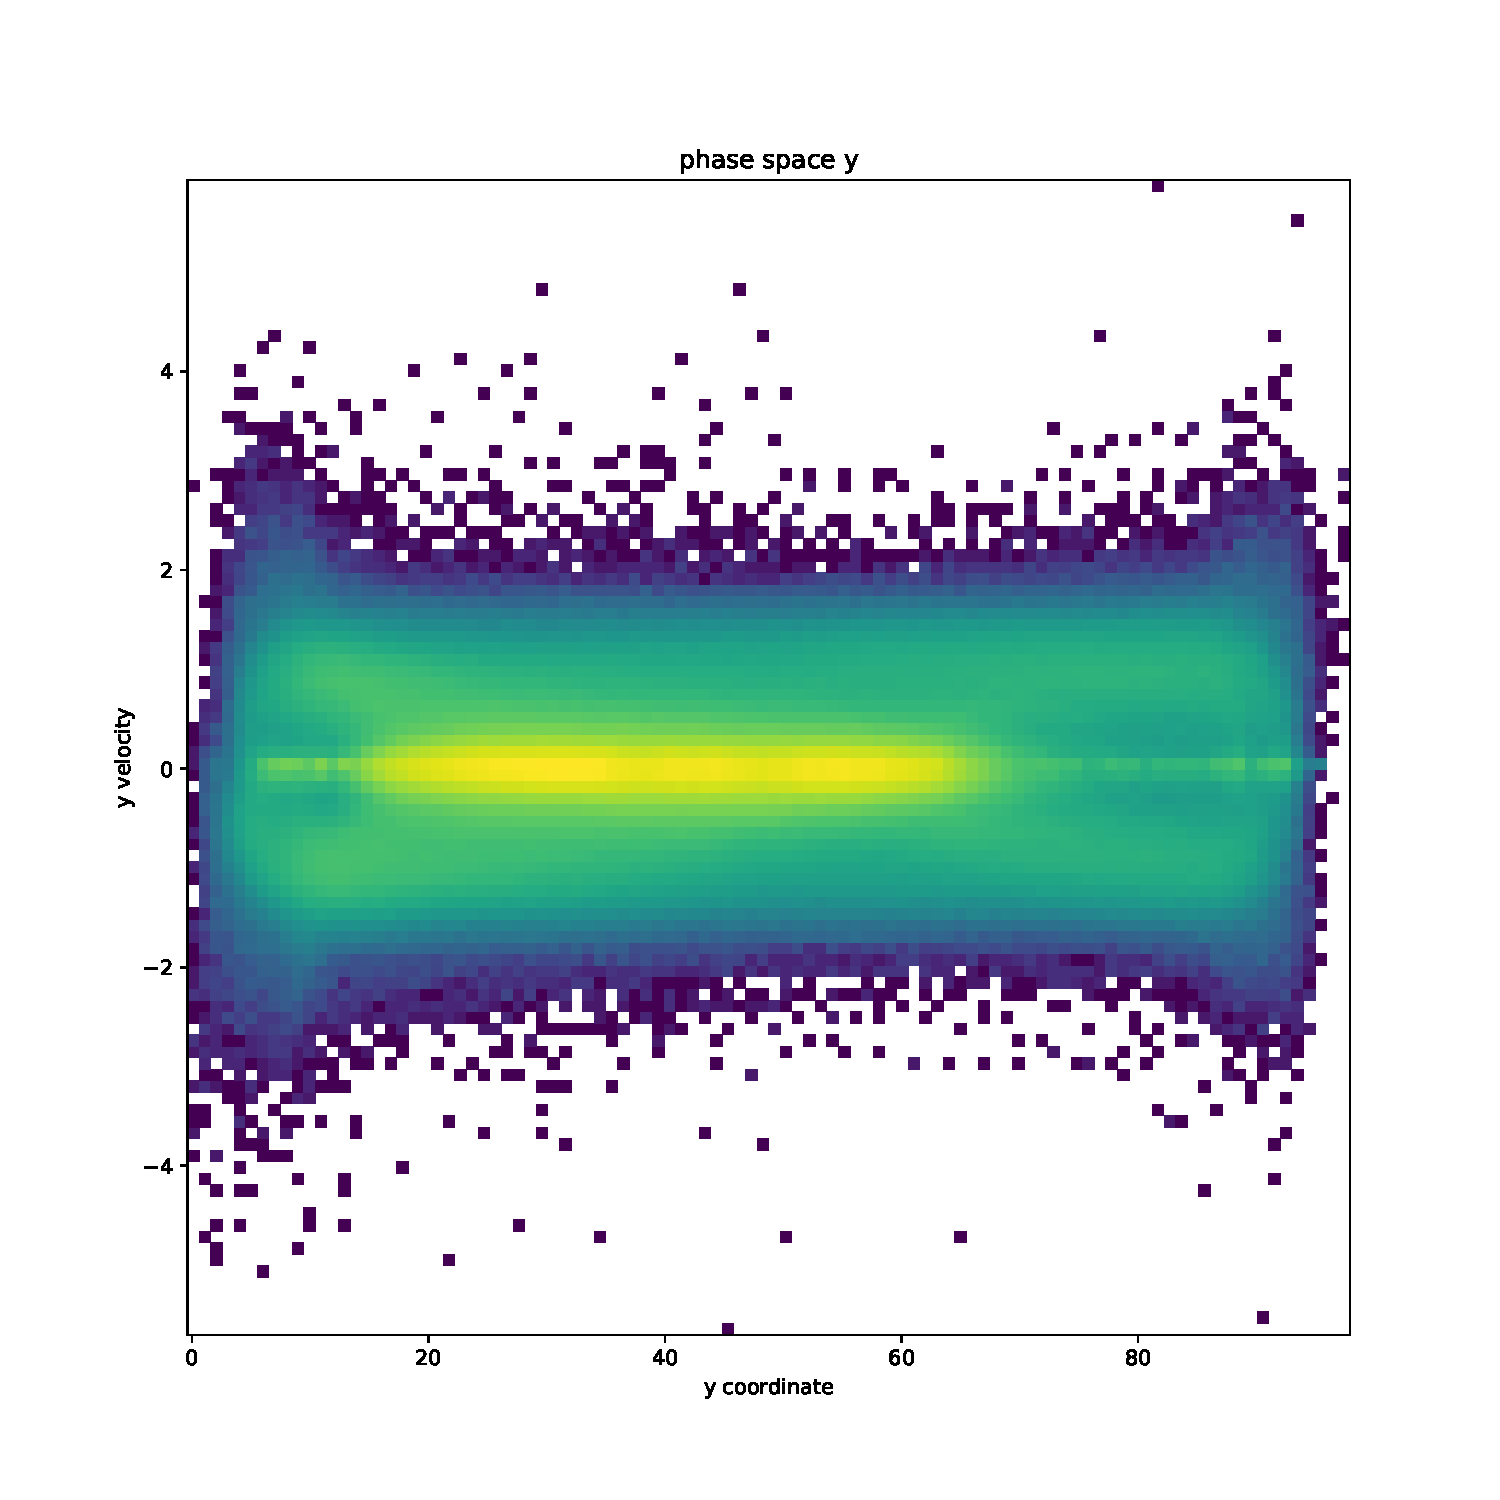
\includegraphics[ width=0.3\textwidth]{fig/hist2d_yvy/save_trainf10_pro_RealData_hist2d_y_vy}
    }\quad\quad
    \subfloat[(iv) Simulation data hist2d yVy]{
        \label{fig:yVy_SimD2Q9Q9}
        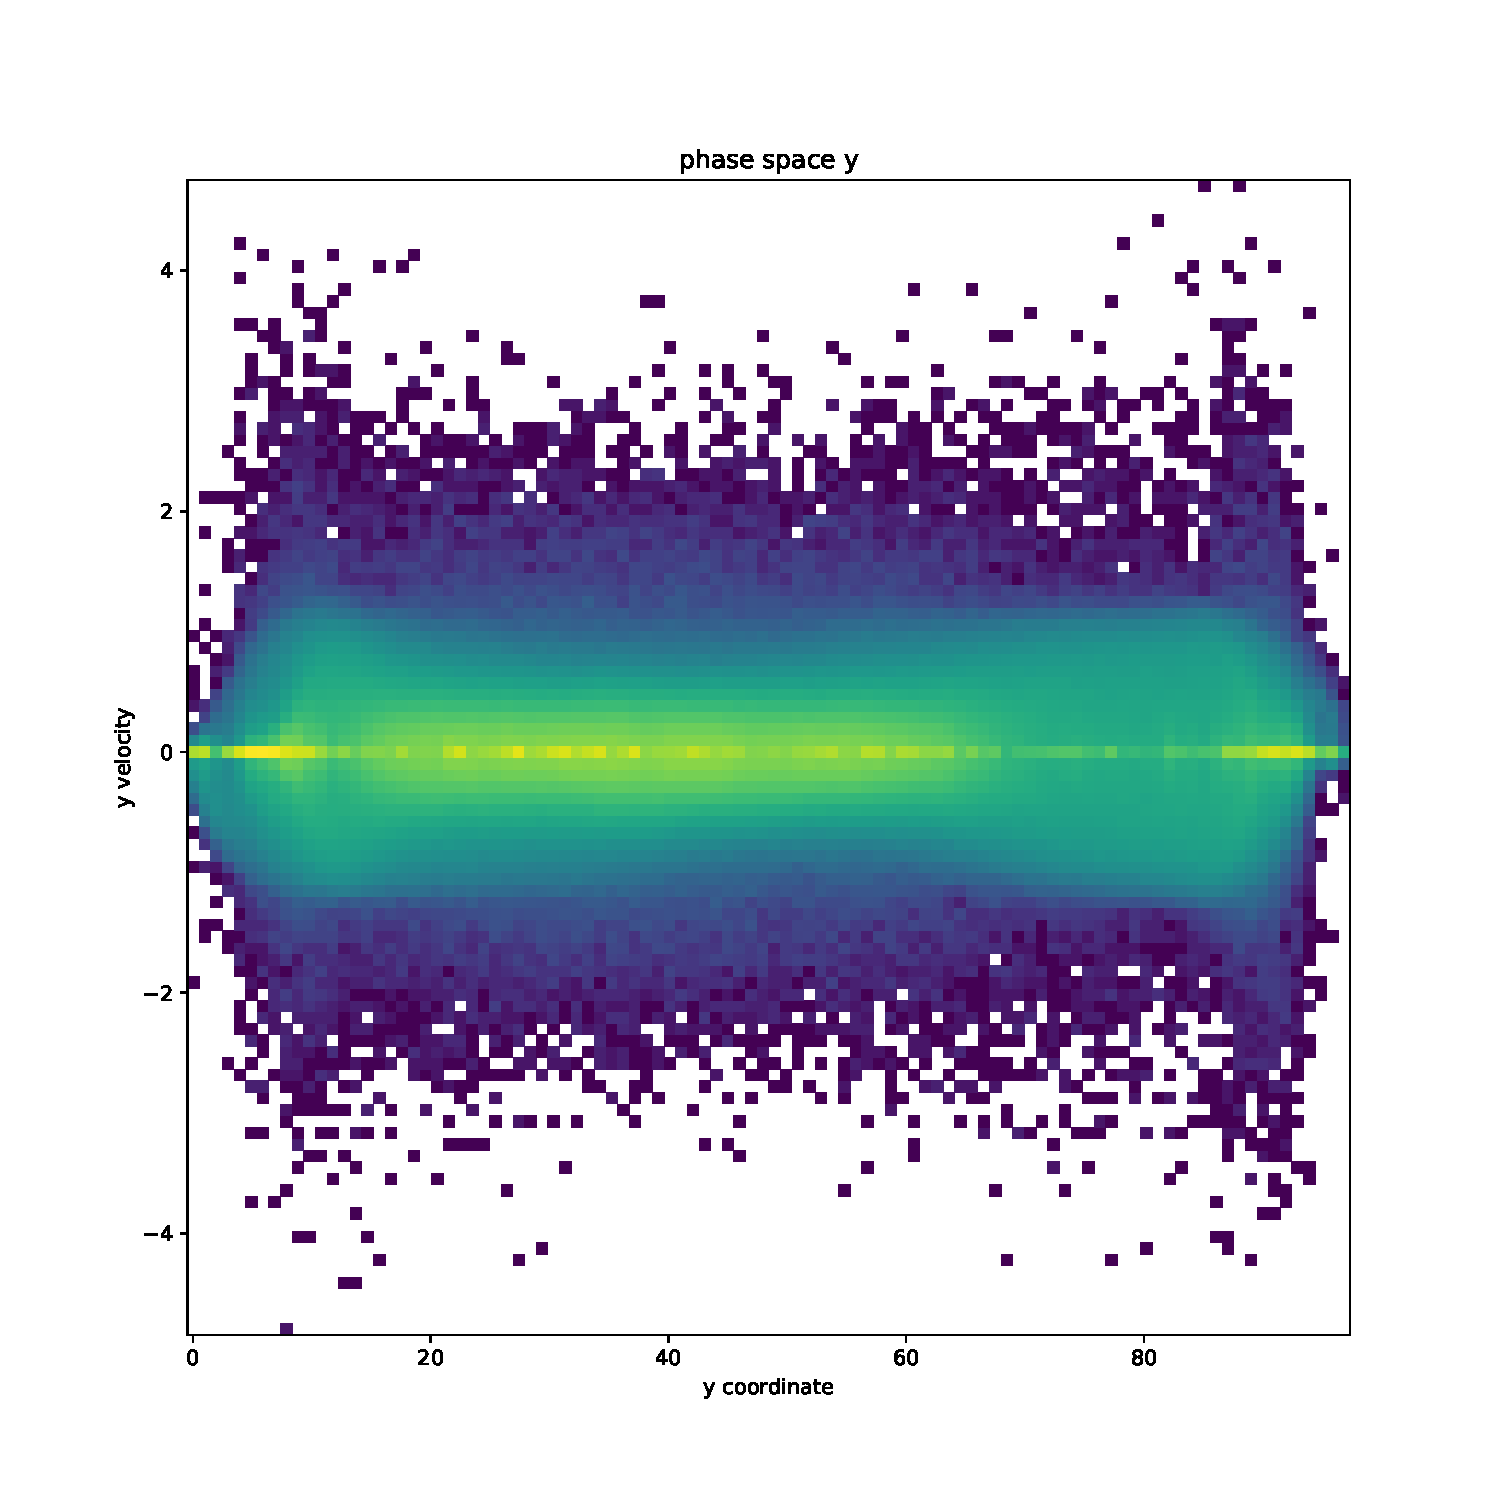
\includegraphics[ width=0.3\textwidth]{fig/hist2d_yvy/save_trainf10_pro_simD2Q9Q9_hist2d_y_vy}
    }
    \caption{(iii) \& (iv) - simD2Q9Q9 - The correlation between the position along the $\vec x$ and $\vec y$ axis and the magnitude of the velocity vector along the same correspondent axes, plotted as heat-map or 2-dimensional histograms.}
        \label{fig:hist2d_SimD2Q9Q9}
\end{figure}
% --------------------------------------
\begin{figure}[!htb]
    \centering
        \subfloat[(v) Real data hist2d Pxy]{
        \label{fig:Pxy_Real_v}
        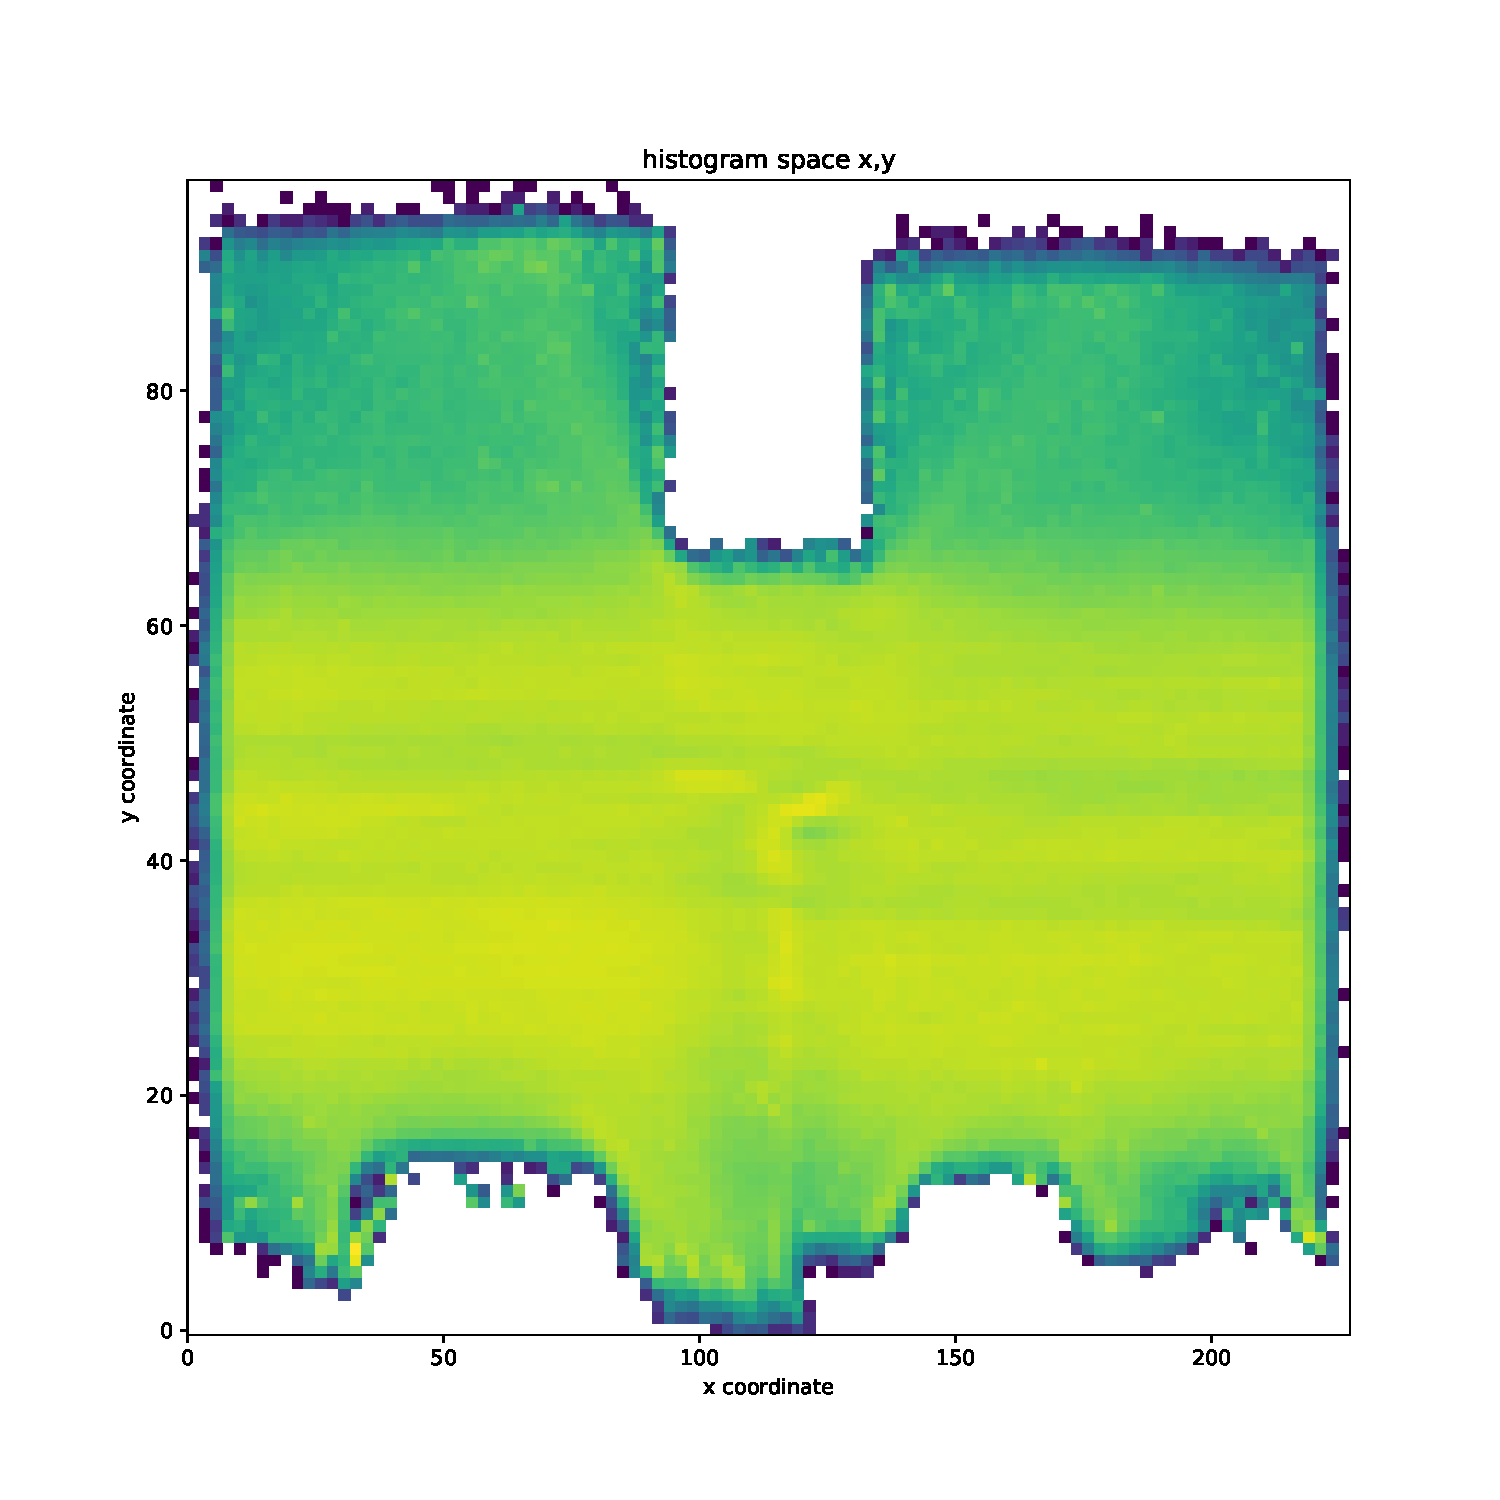
\includegraphics[ width=0.3\textwidth]{fig/hist2d_pxy/save_trainf10_pro_RealData_hist2d_x_y}
    }\quad\quad
    \subfloat[(v) Simulation data hist2d Pxy]{
        \label{fig:Pxy_SimD2Q9Q9}
        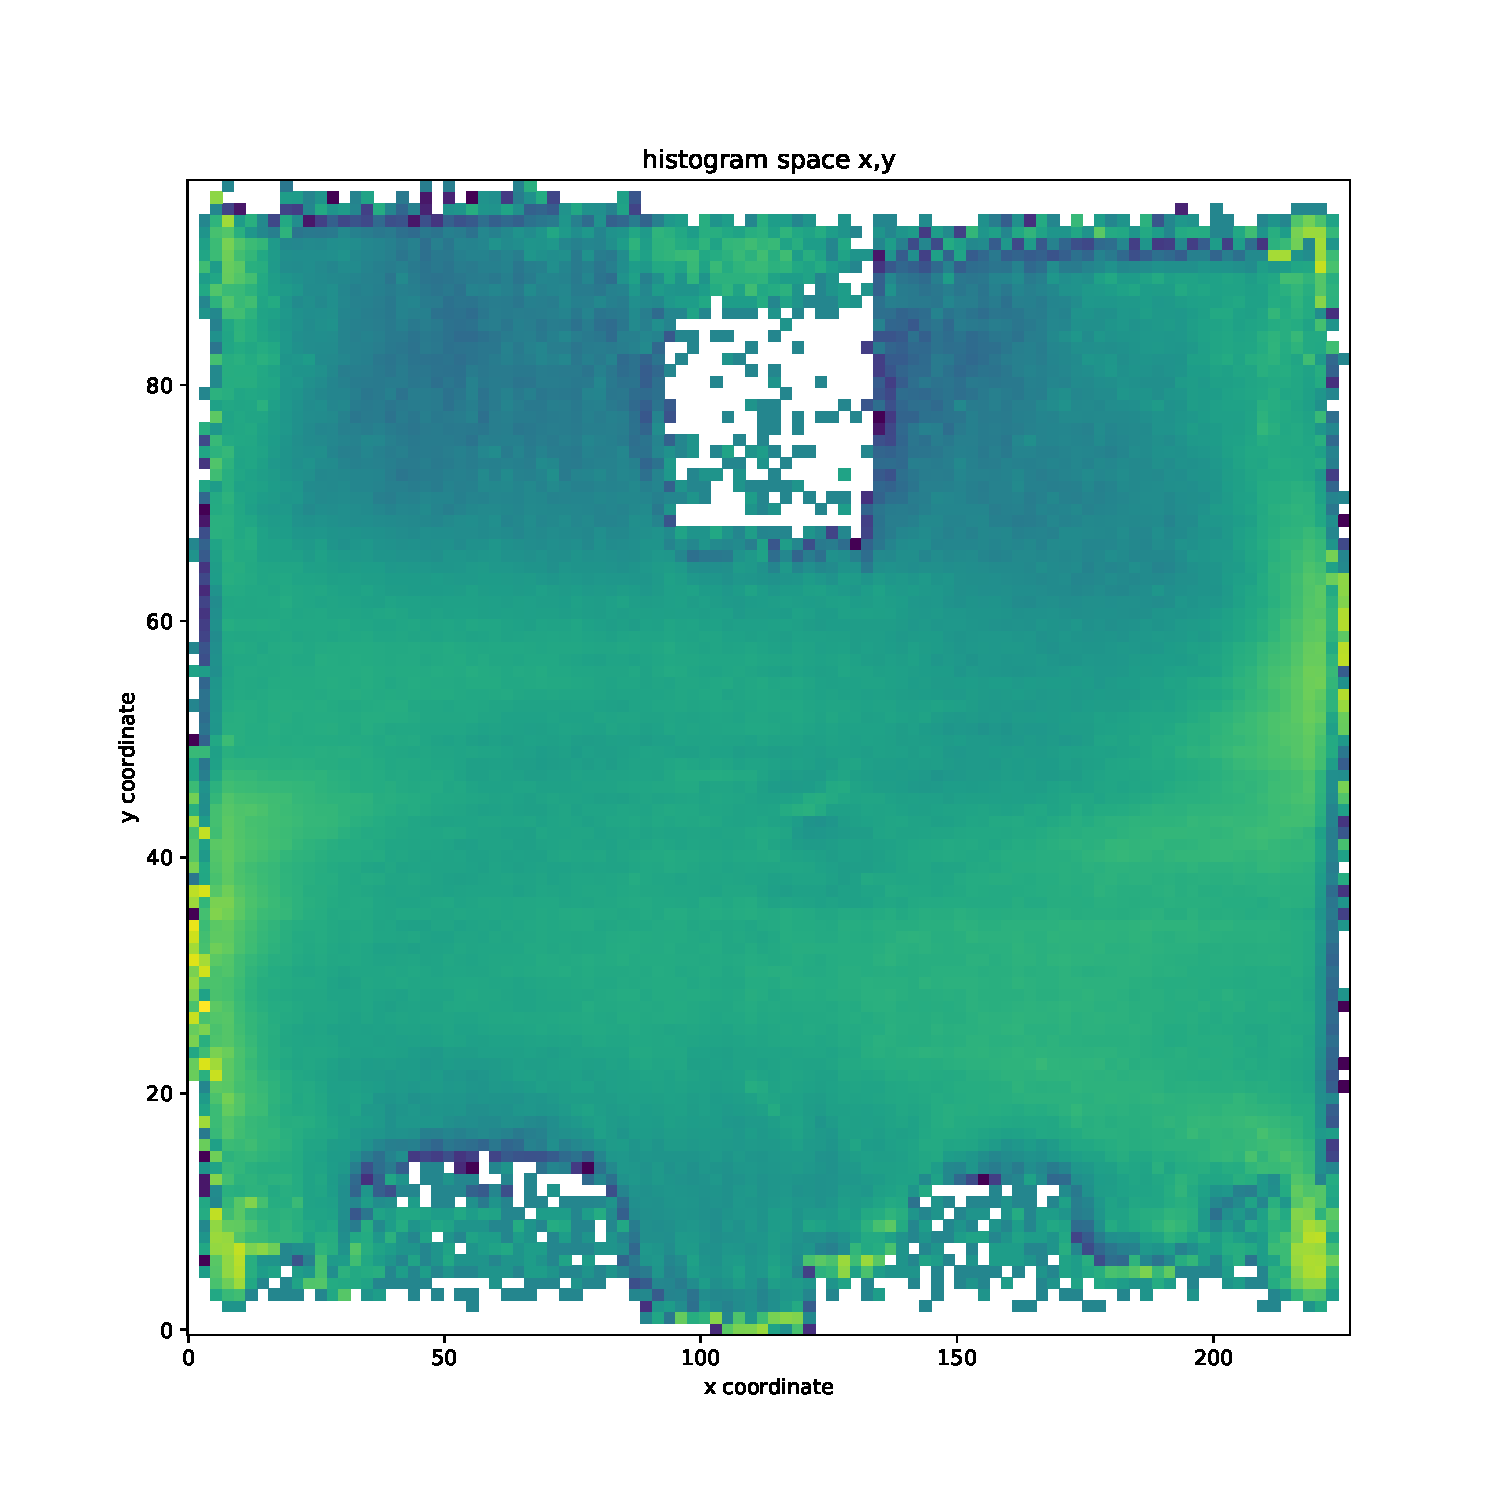
\includegraphics[ width=0.3\textwidth]{fig/hist2d_pxy/save_trainf10_pro_simD2Q9Q9_hist2d_x_y}
    }
    \caption{(v) - simD2Q9Q9 - The heat-map of the positions along $\vec x$ and $\vec y$ axis of all paths that have passed though, plotted as 2-dimensional histogram.}
    \label{fig:Pxy_SimD2Q9Q9}
\end{figure}


\FloatBarrier
% -------------------------------------------------------------------------------------------------------------------------------------------------------------------------------------------
\subsection{Real data - TD2Q9}
This paragraph's reference are the following: (Figure \ref{fig:hist_SimTD2Q9}), (Figure \ref{fig:hist2d_SimTD2Q9}), (Figure \ref{fig:Pxy_SimTD2Q9}) 

\begin{figure}[!htb]
    \centering
    \subfloat[(i) Real data hist vx]{
        \label{fig:Vx_Real_i}
        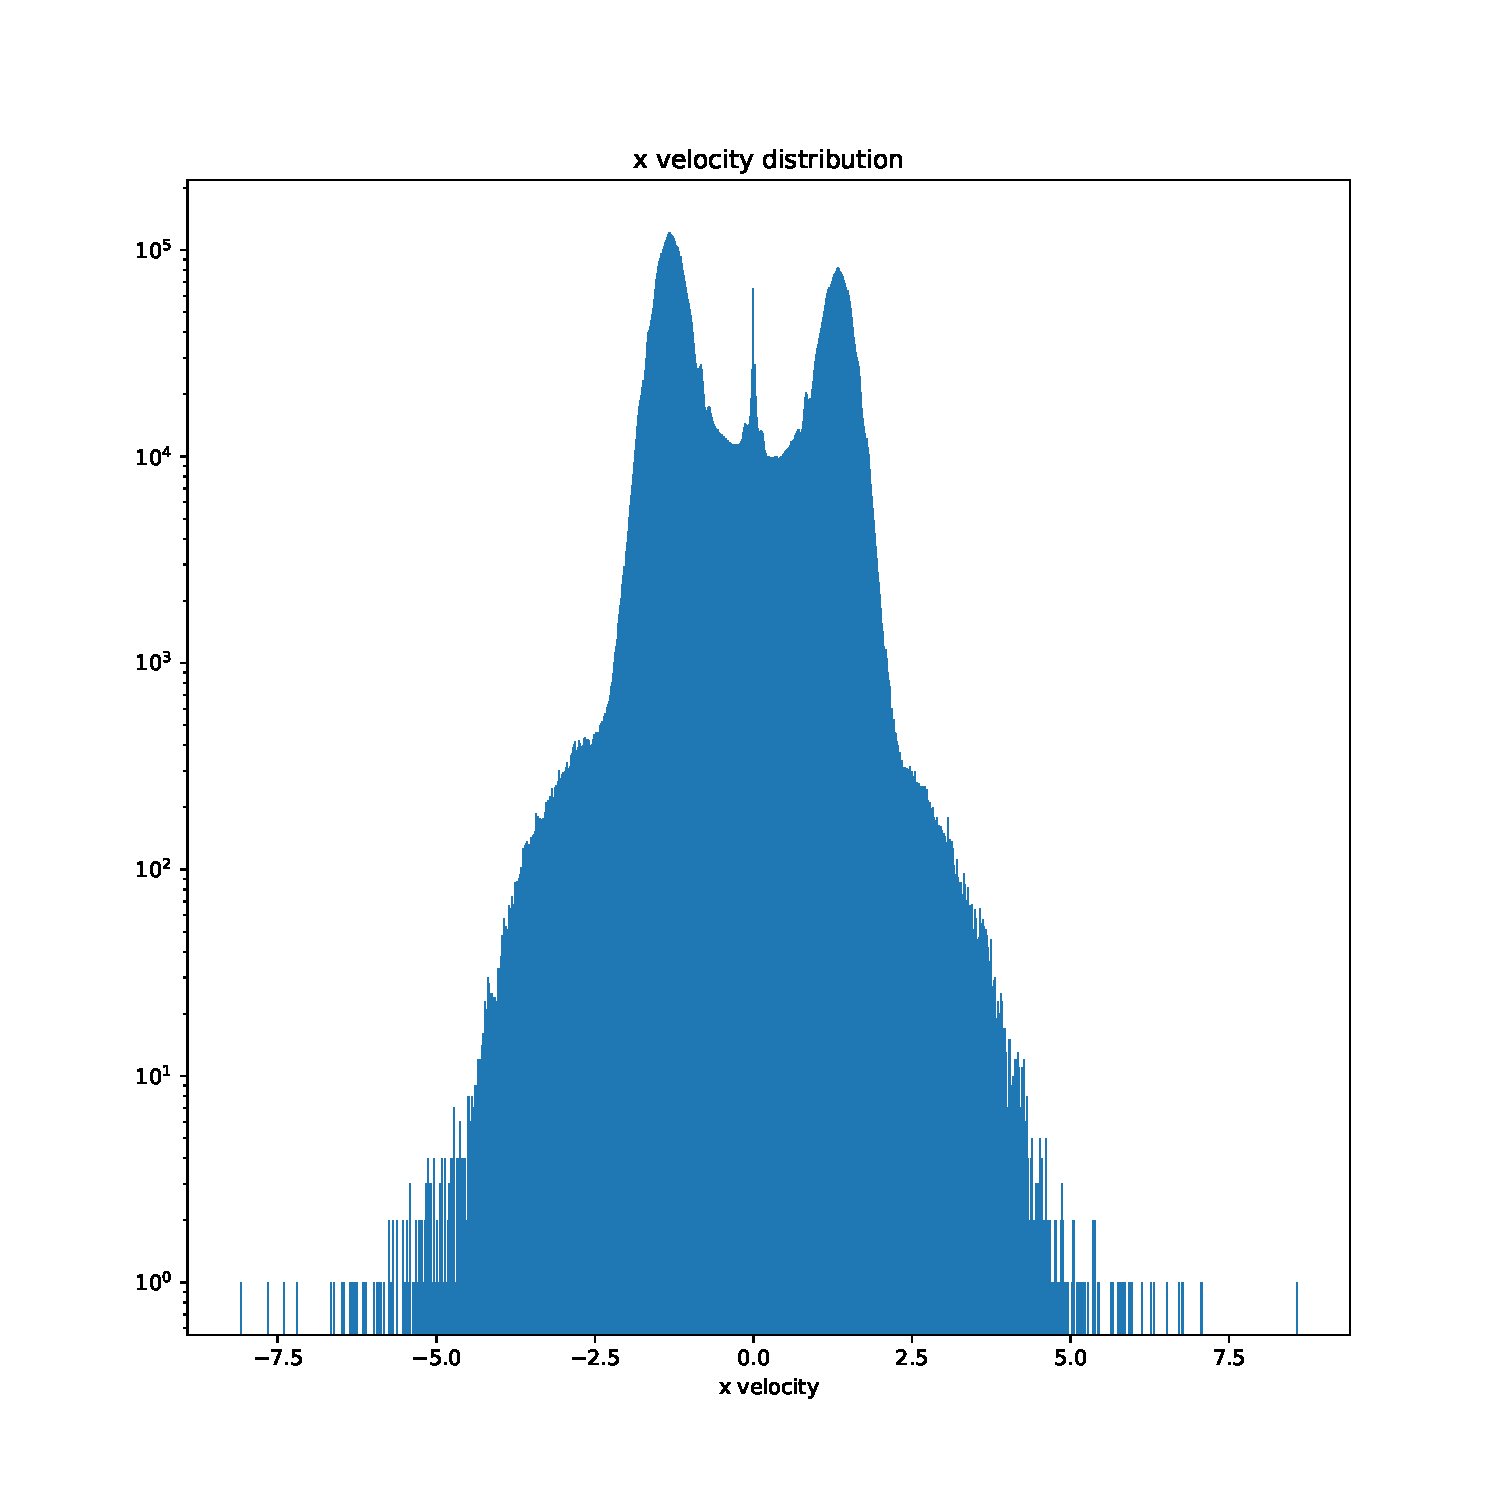
\includegraphics[ width=0.3\textwidth]{fig/hist_vx/save_trainf10_pro_RealData_hist_vx}
    }\quad\quad
    \subfloat[(i) Simulation data hist vx]{
        \label{fig:Vx_SimTD2Q9}
        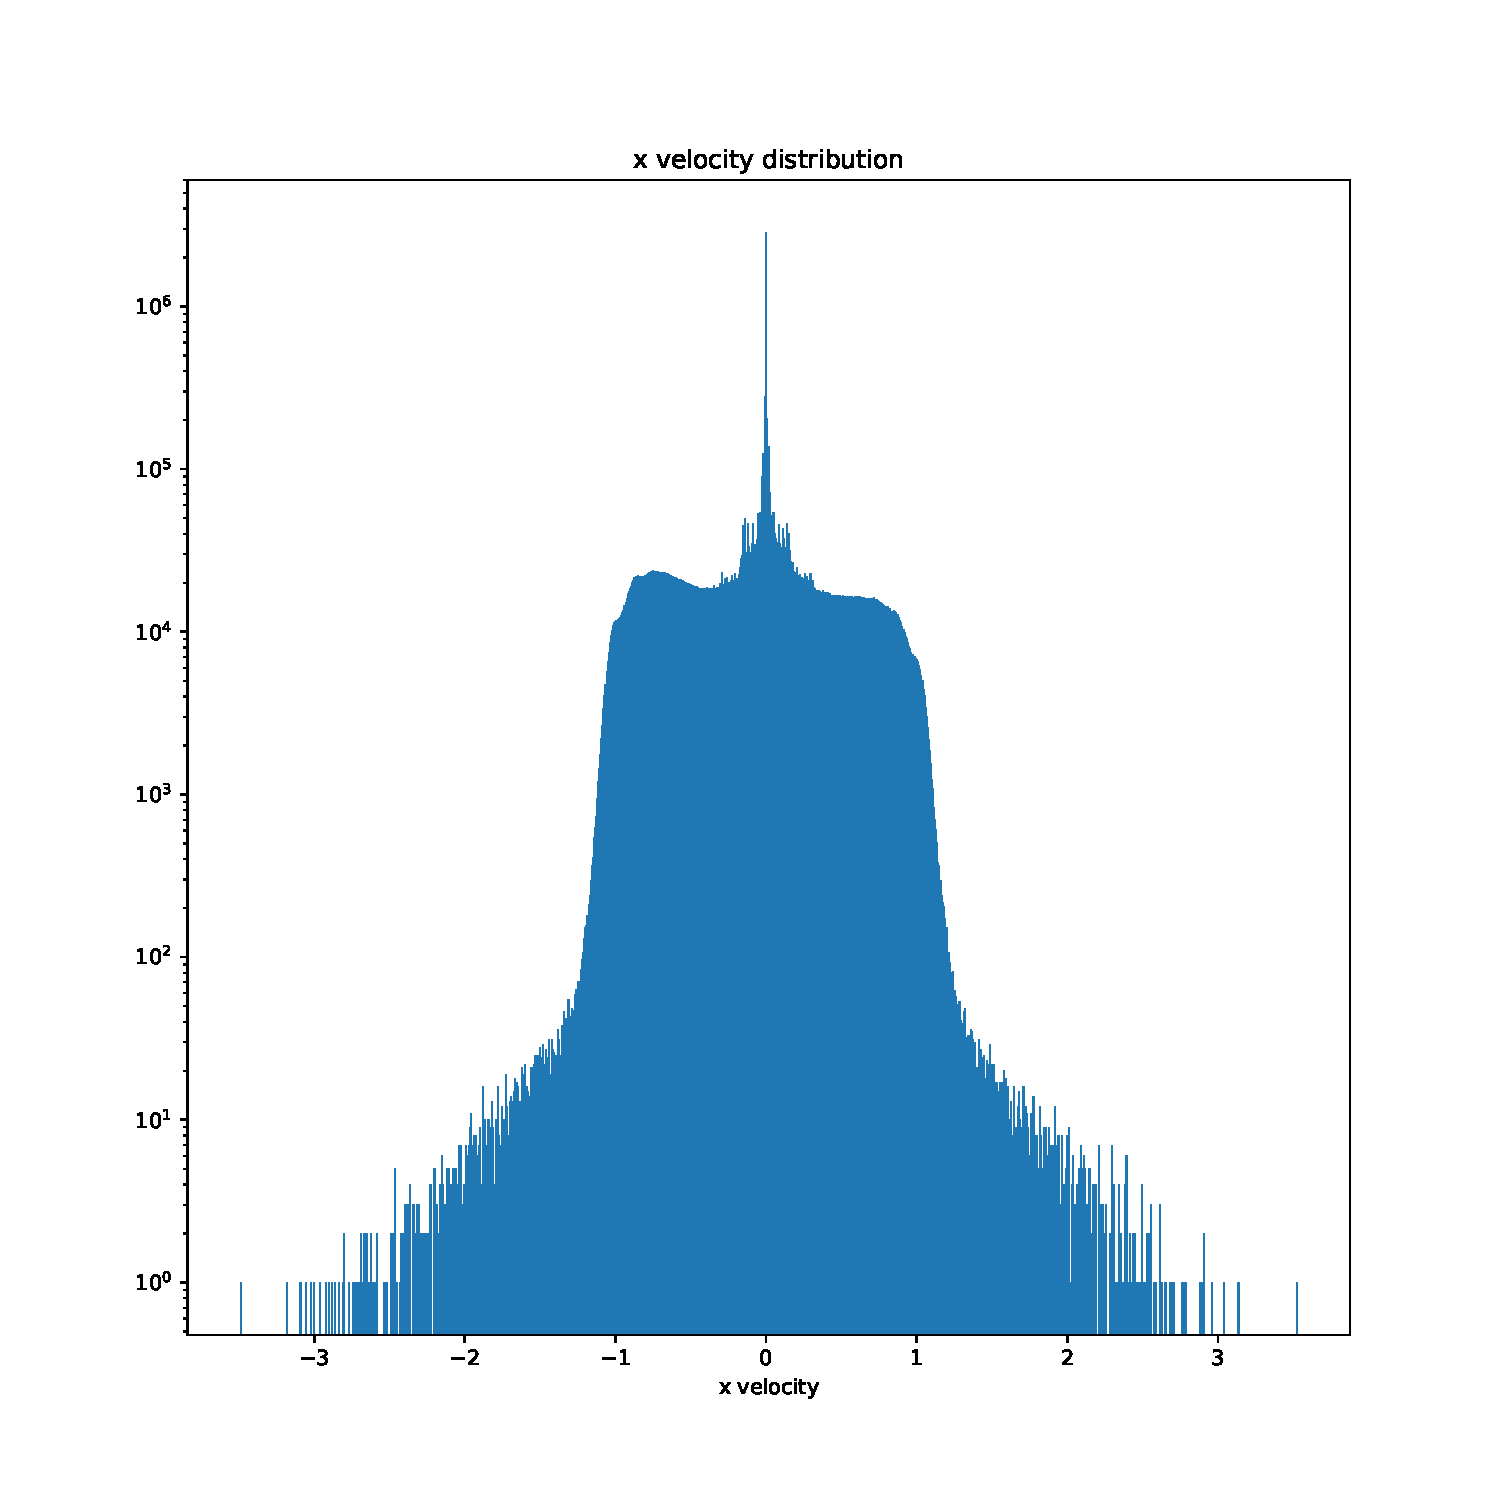
\includegraphics[ width=0.3\textwidth]{fig/hist_vx/save_trainf10_pro_simTD2Q9_hist_vx}
    }\quad\quad
    \subfloat[(ii) Real data hist vy]{
        \label{fig:Vy_Real_ii}
        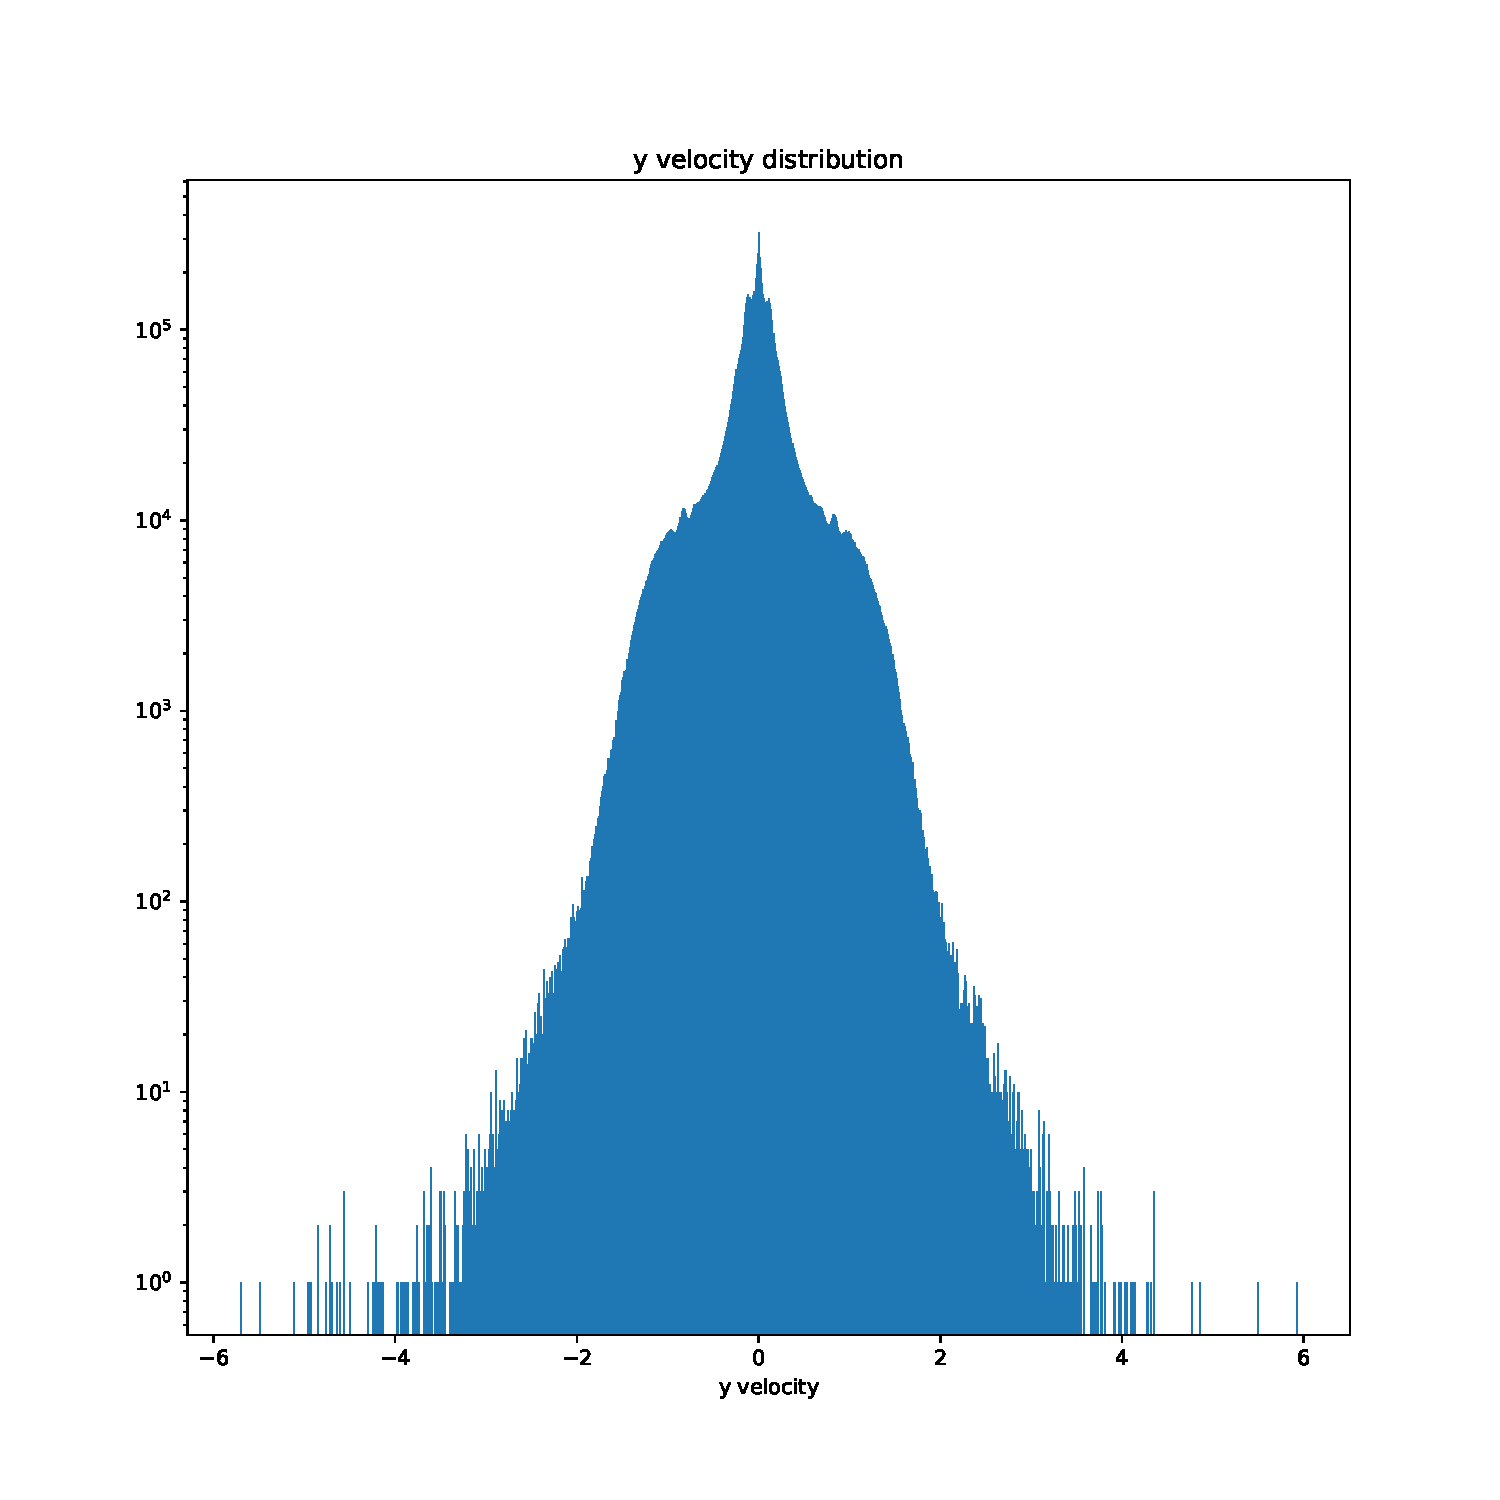
\includegraphics[ width=0.3\textwidth]{fig/hist_vy/save_trainf10_pro_RealData_hist_vy}
    }\quad\quad
    \subfloat[(ii) Simulation data hist vy]{
        \label{fig:Vy_SimTD2Q9}
        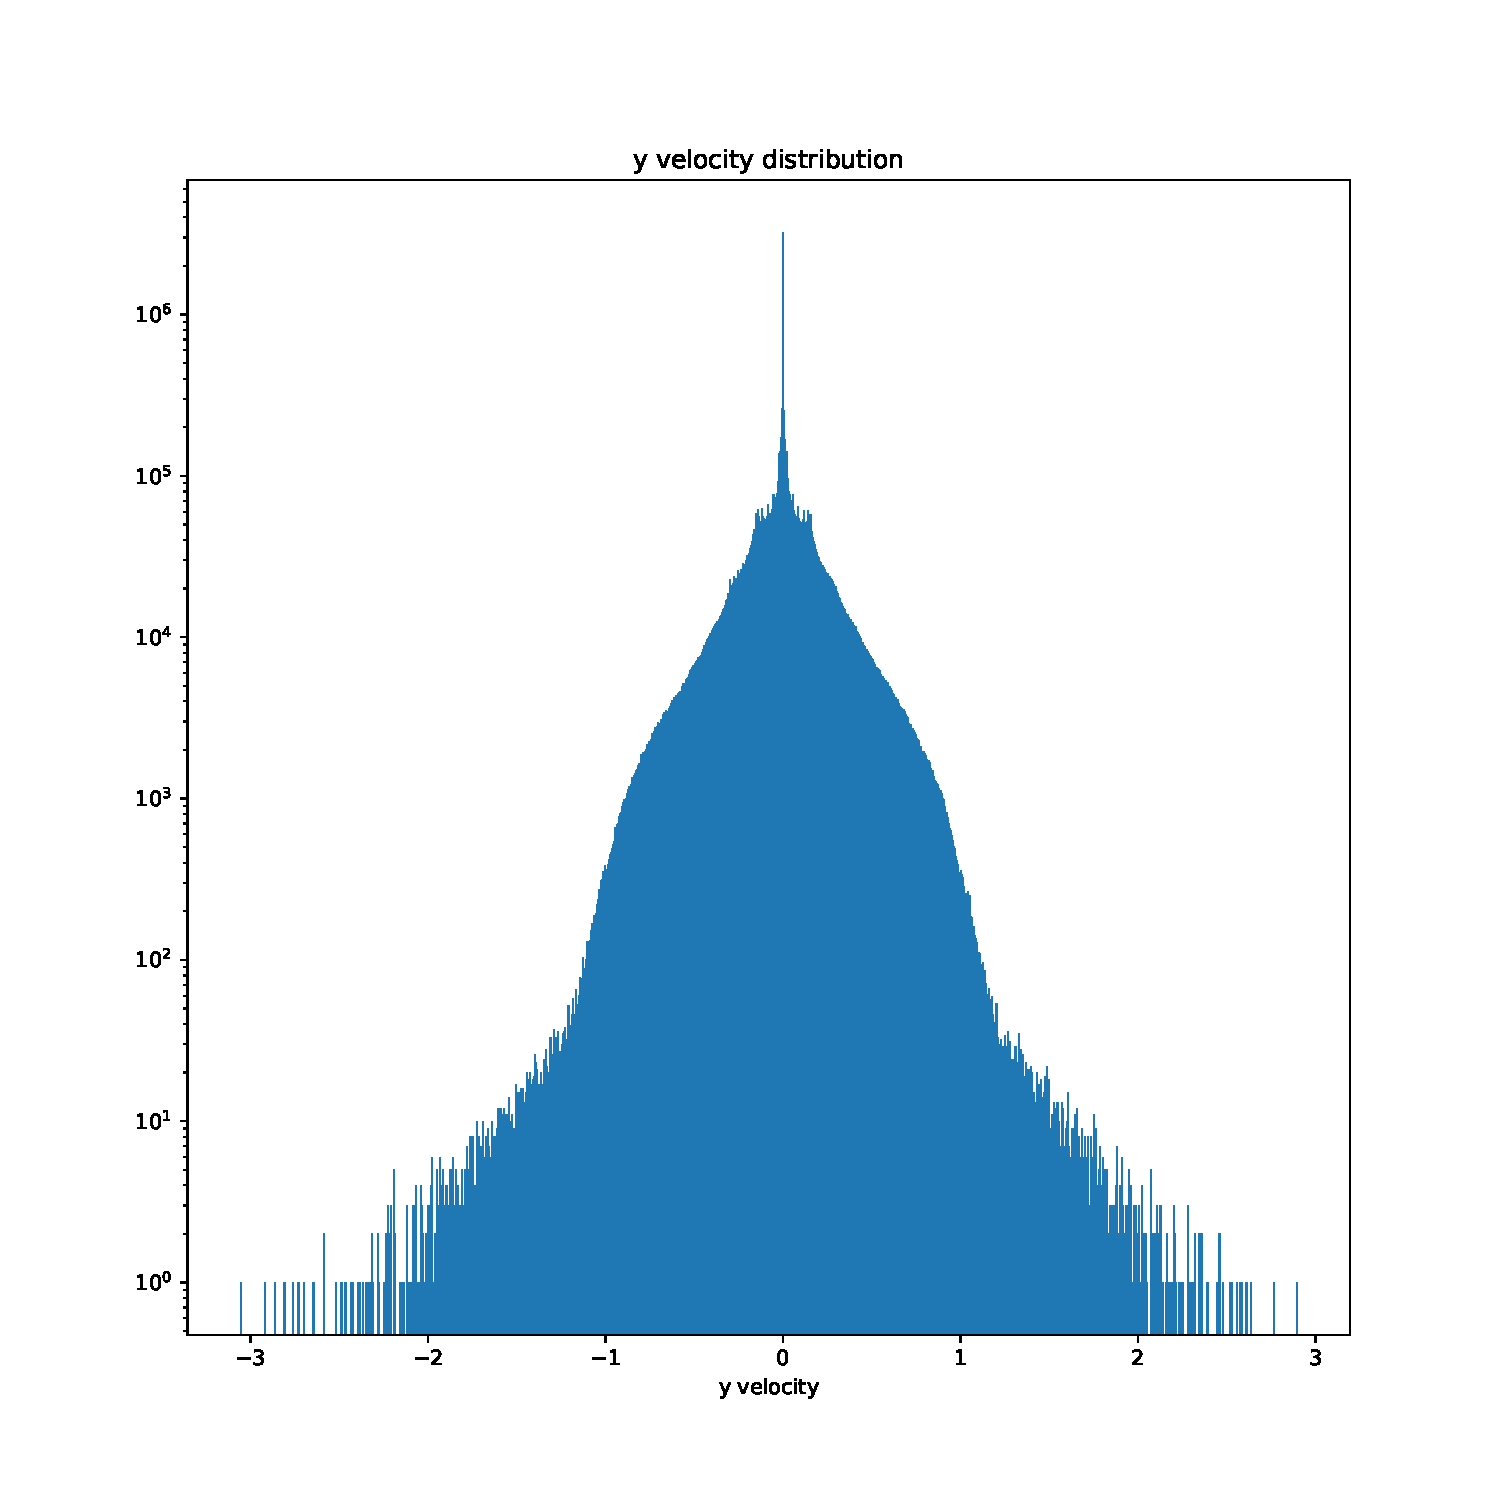
\includegraphics[ width=0.3\textwidth]{fig/hist_vy/save_trainf10_pro_simTD2Q9_hist_vy}
    }
    \caption{(i) \& (ii) - simTD2Q9 - The magnitude of the velocity vector along the $\vec x$ and $\vec y$ axis, plotted as 1-dimensional histograms.}
    \label{fig:hist_SimTD2Q9}
\end{figure}
% --------------------------------------
\begin{figure}[!htb]
    \centering
        \subfloat[(iii) Real data hist2d xVx]{
        \label{fig:xVx_Real_iii}
        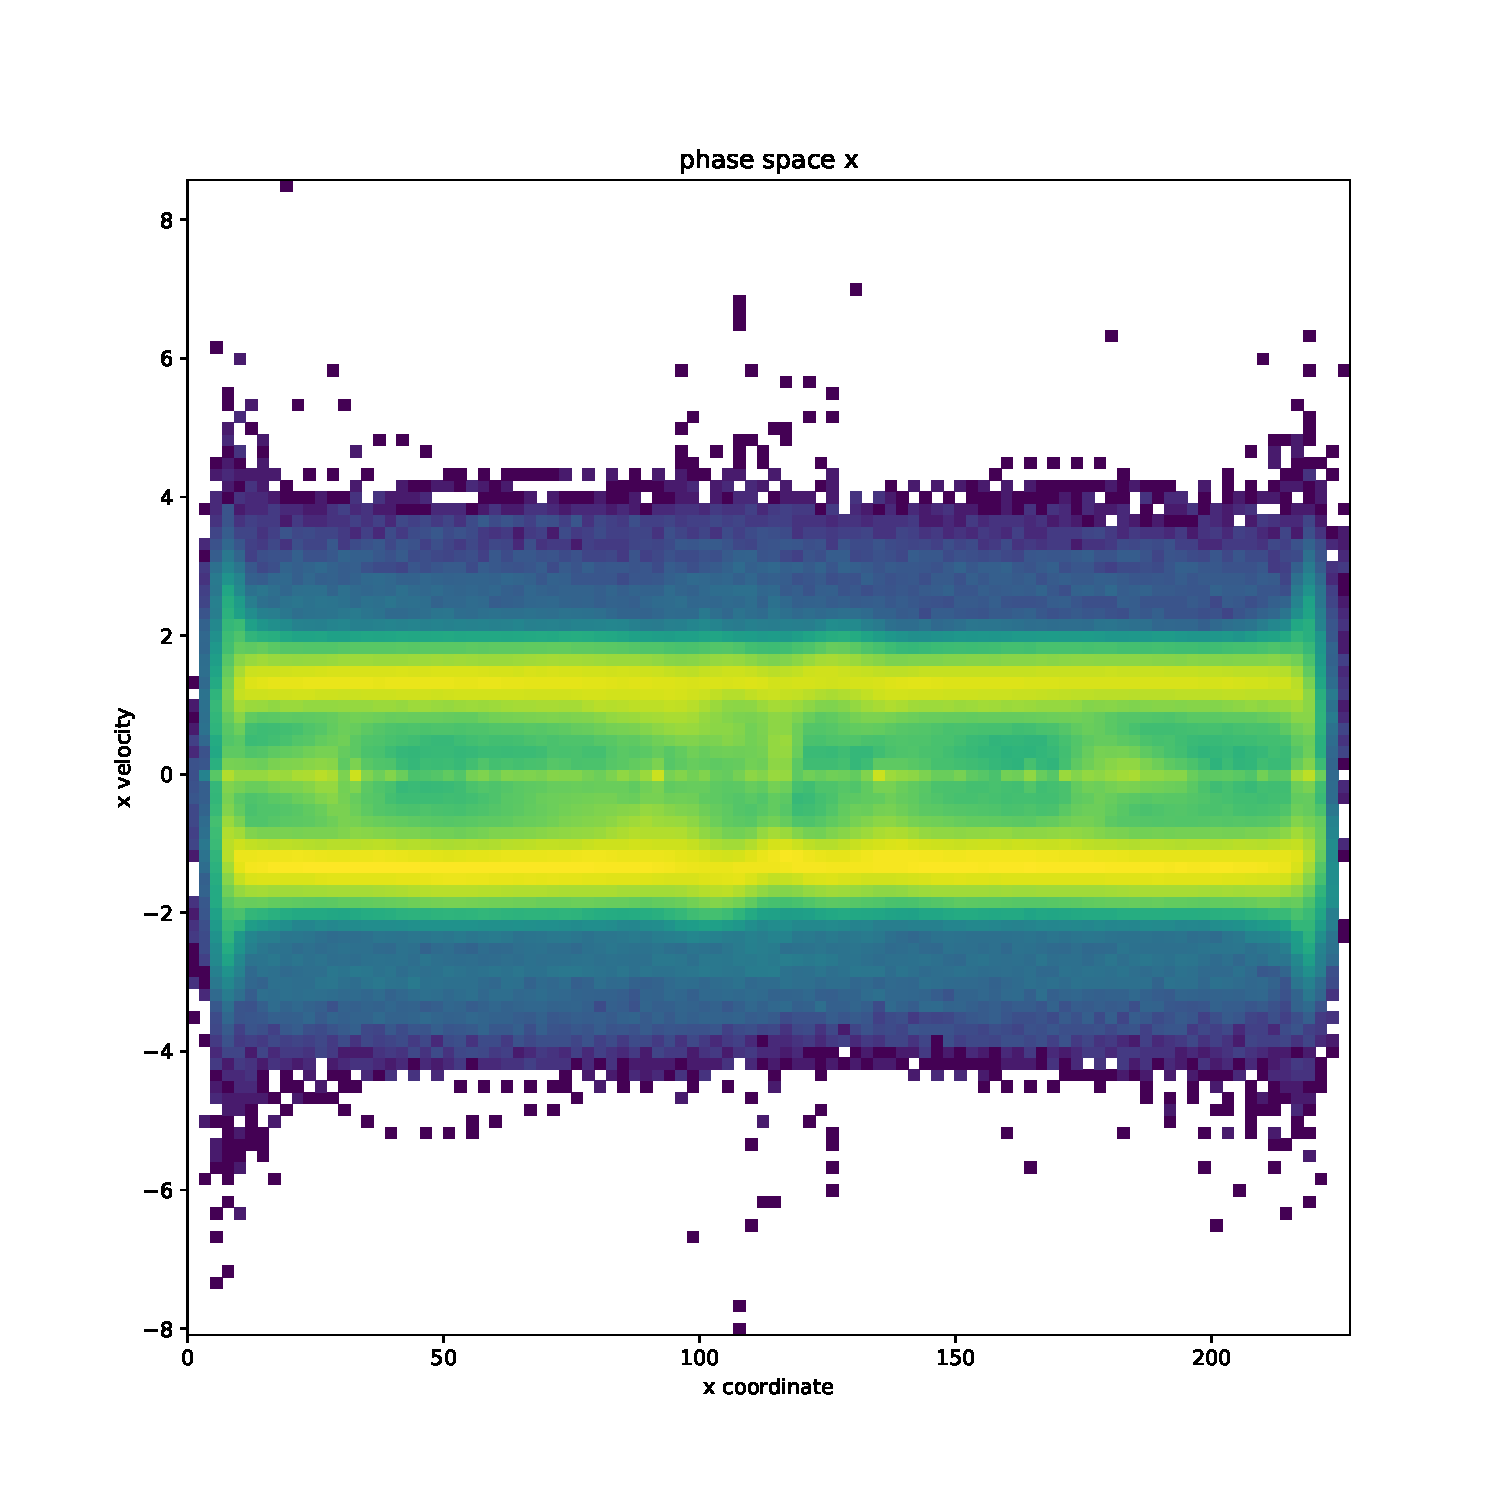
\includegraphics[ width=0.3\textwidth]{fig/hist2d_xvx/save_trainf10_pro_RealData_hist2d_x_vx}
    }\quad\quad
    \subfloat[(iii) Simulation data hist2d xVx]{
        \label{fig:xVx_SimTD2Q9}
        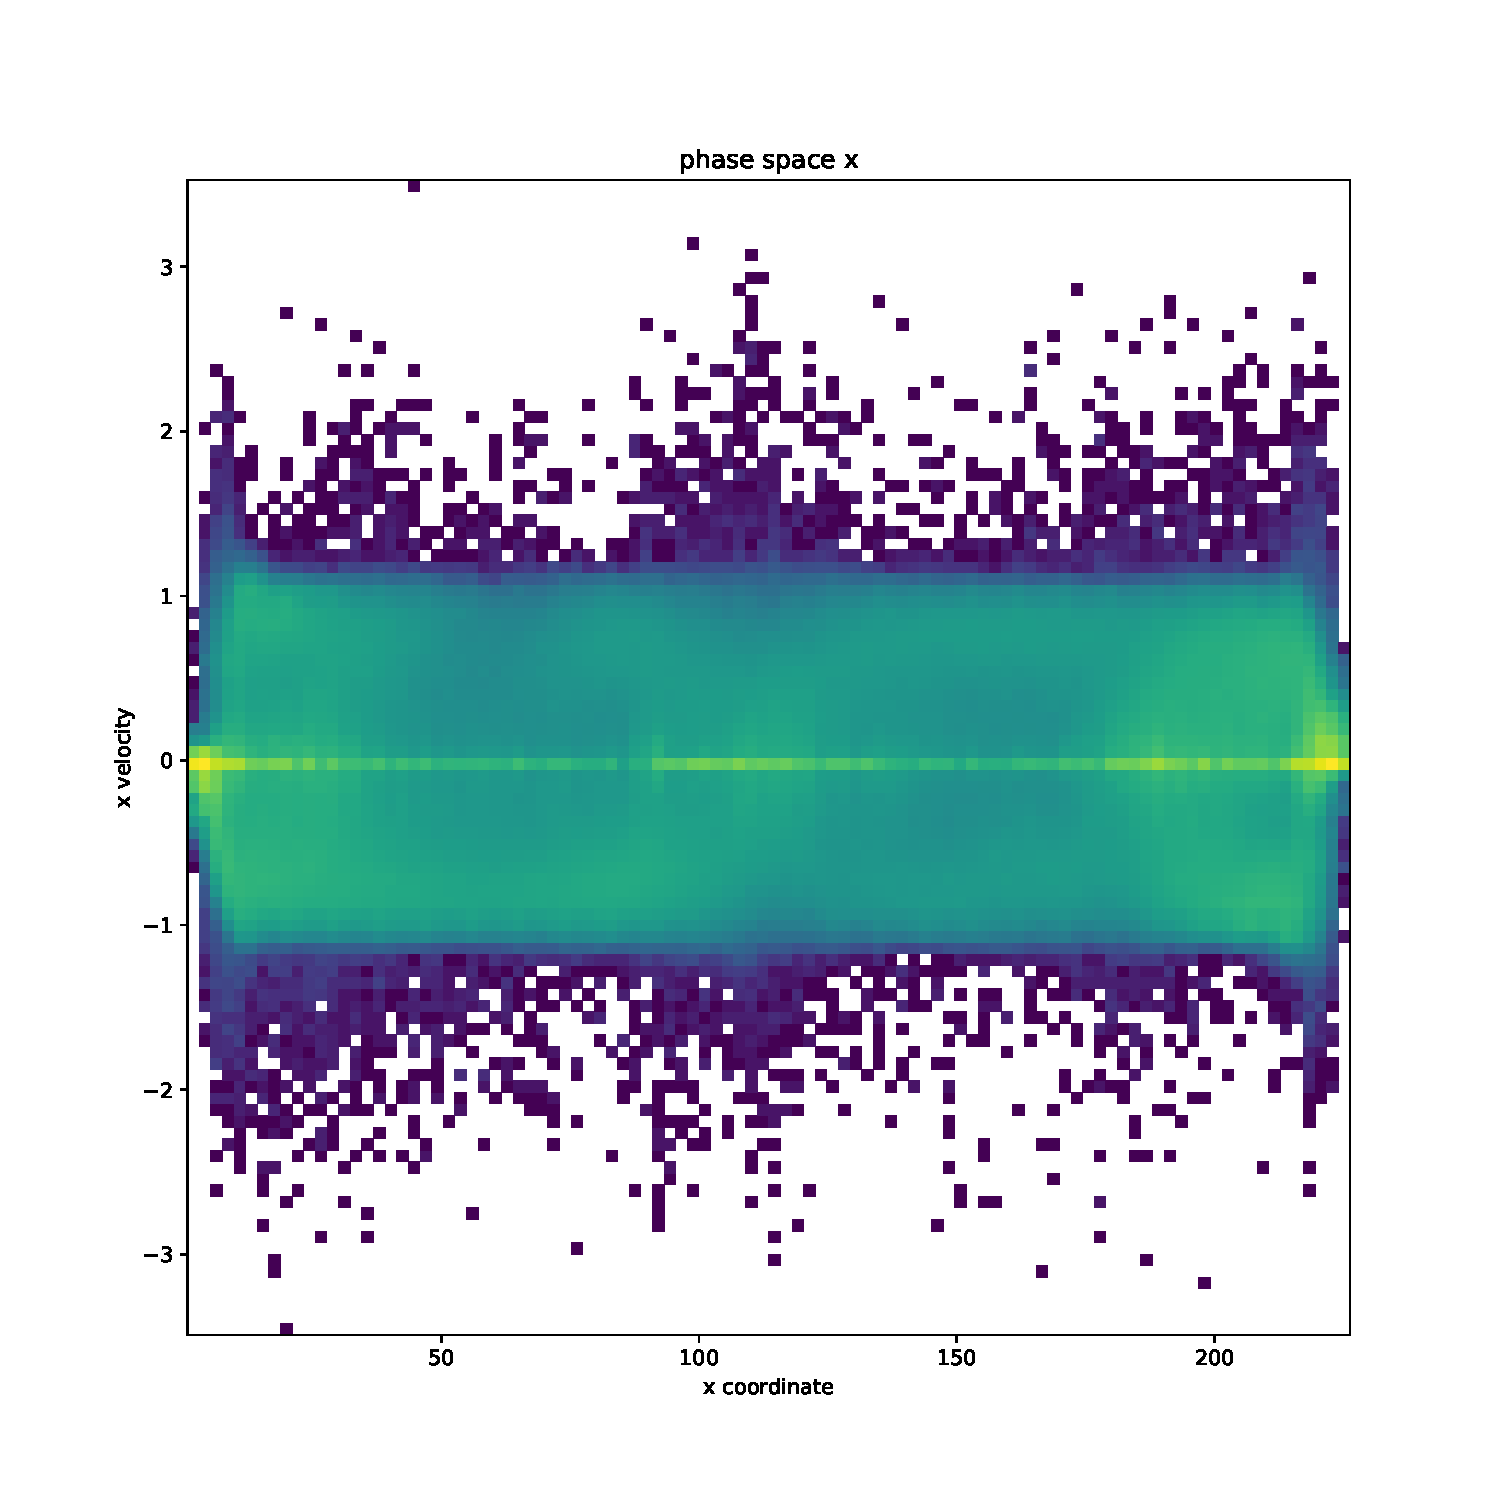
\includegraphics[ width=0.3\textwidth]{fig/hist2d_xvx/save_trainf10_pro_simTD2Q9_hist2d_x_vx}
    }\quad\quad
    \subfloat[(iv) Real data hist2d yVy]{
        \label{fig:yvy_Real_iv}
        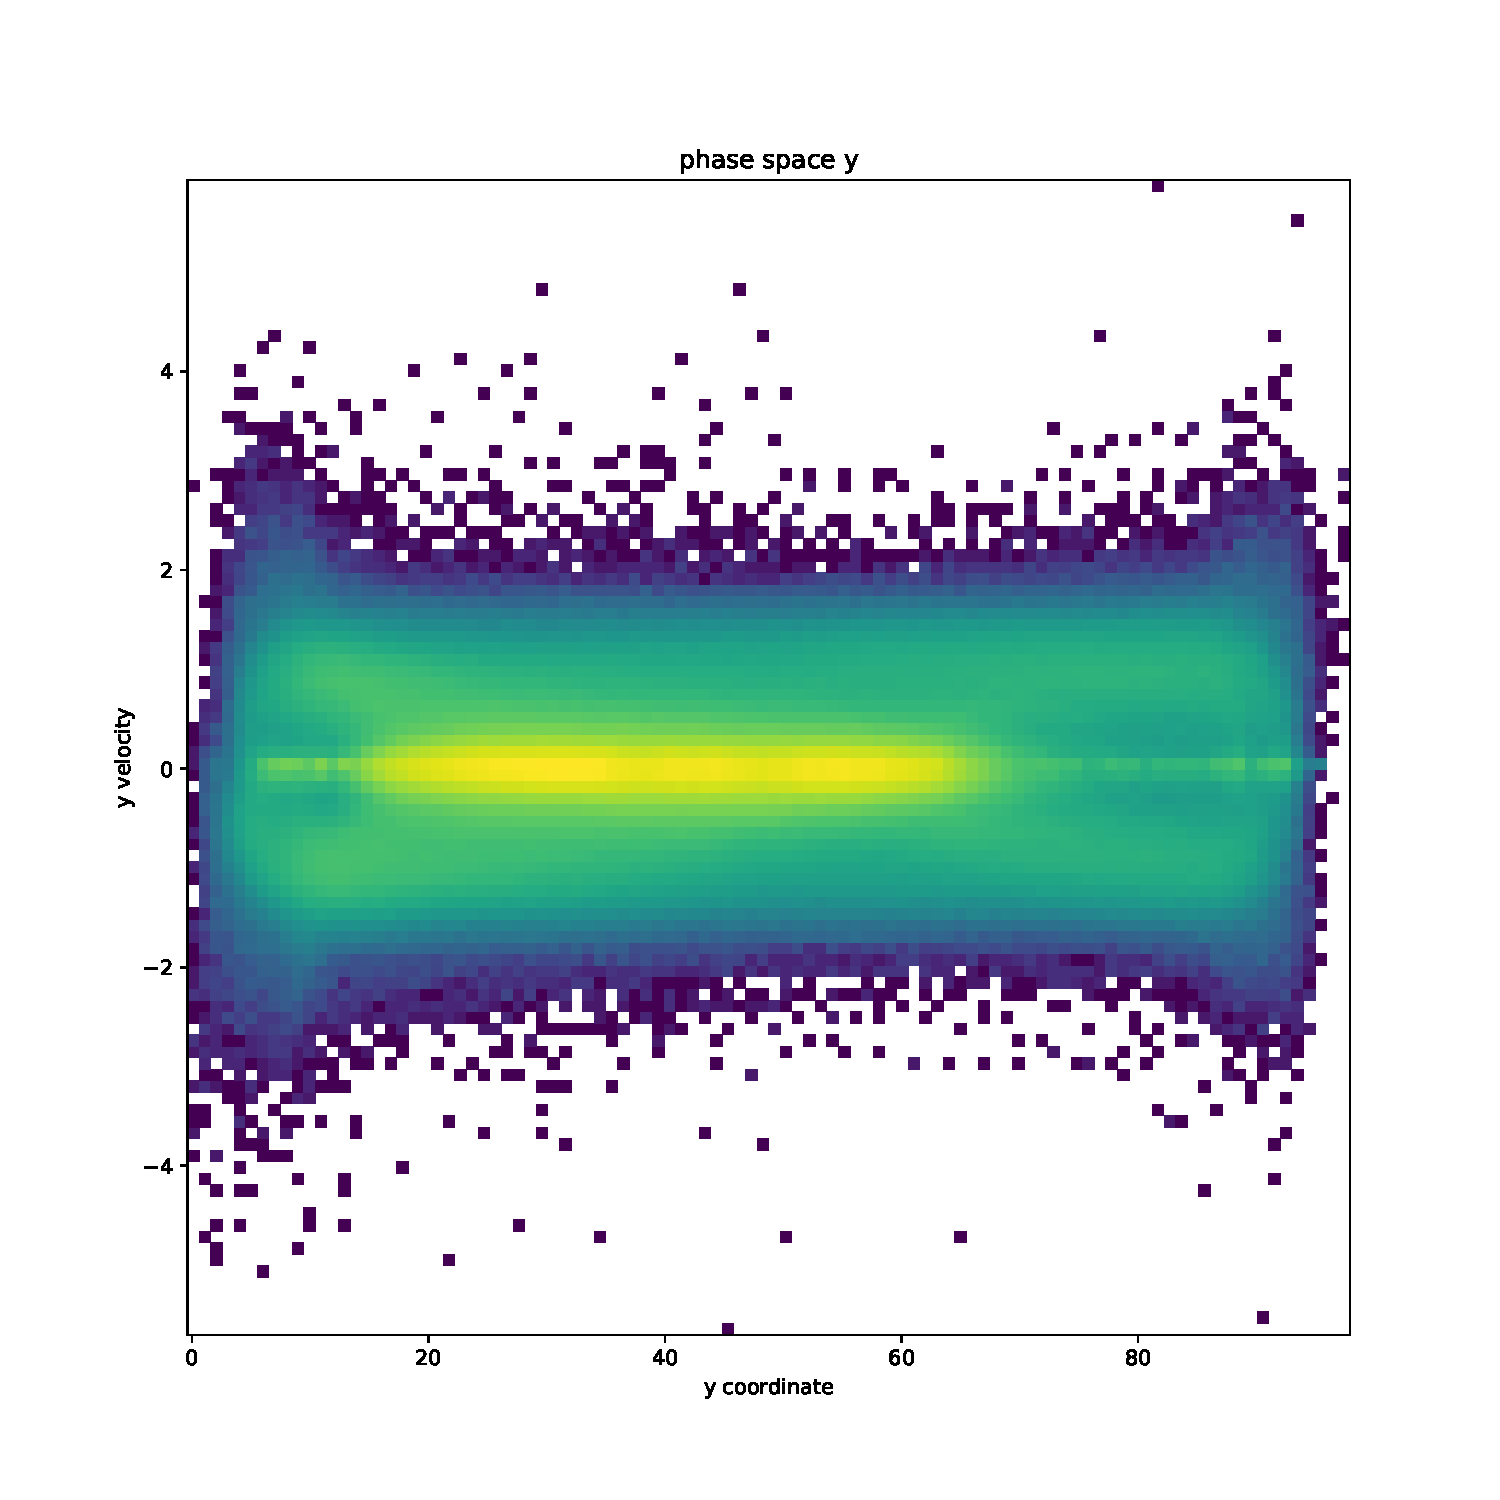
\includegraphics[ width=0.3\textwidth]{fig/hist2d_yvy/save_trainf10_pro_RealData_hist2d_y_vy}
    }\quad\quad
    \subfloat[(iv) Simulation data hist2d yVy]{
        \label{fig:yVy_SimTD2Q9}
        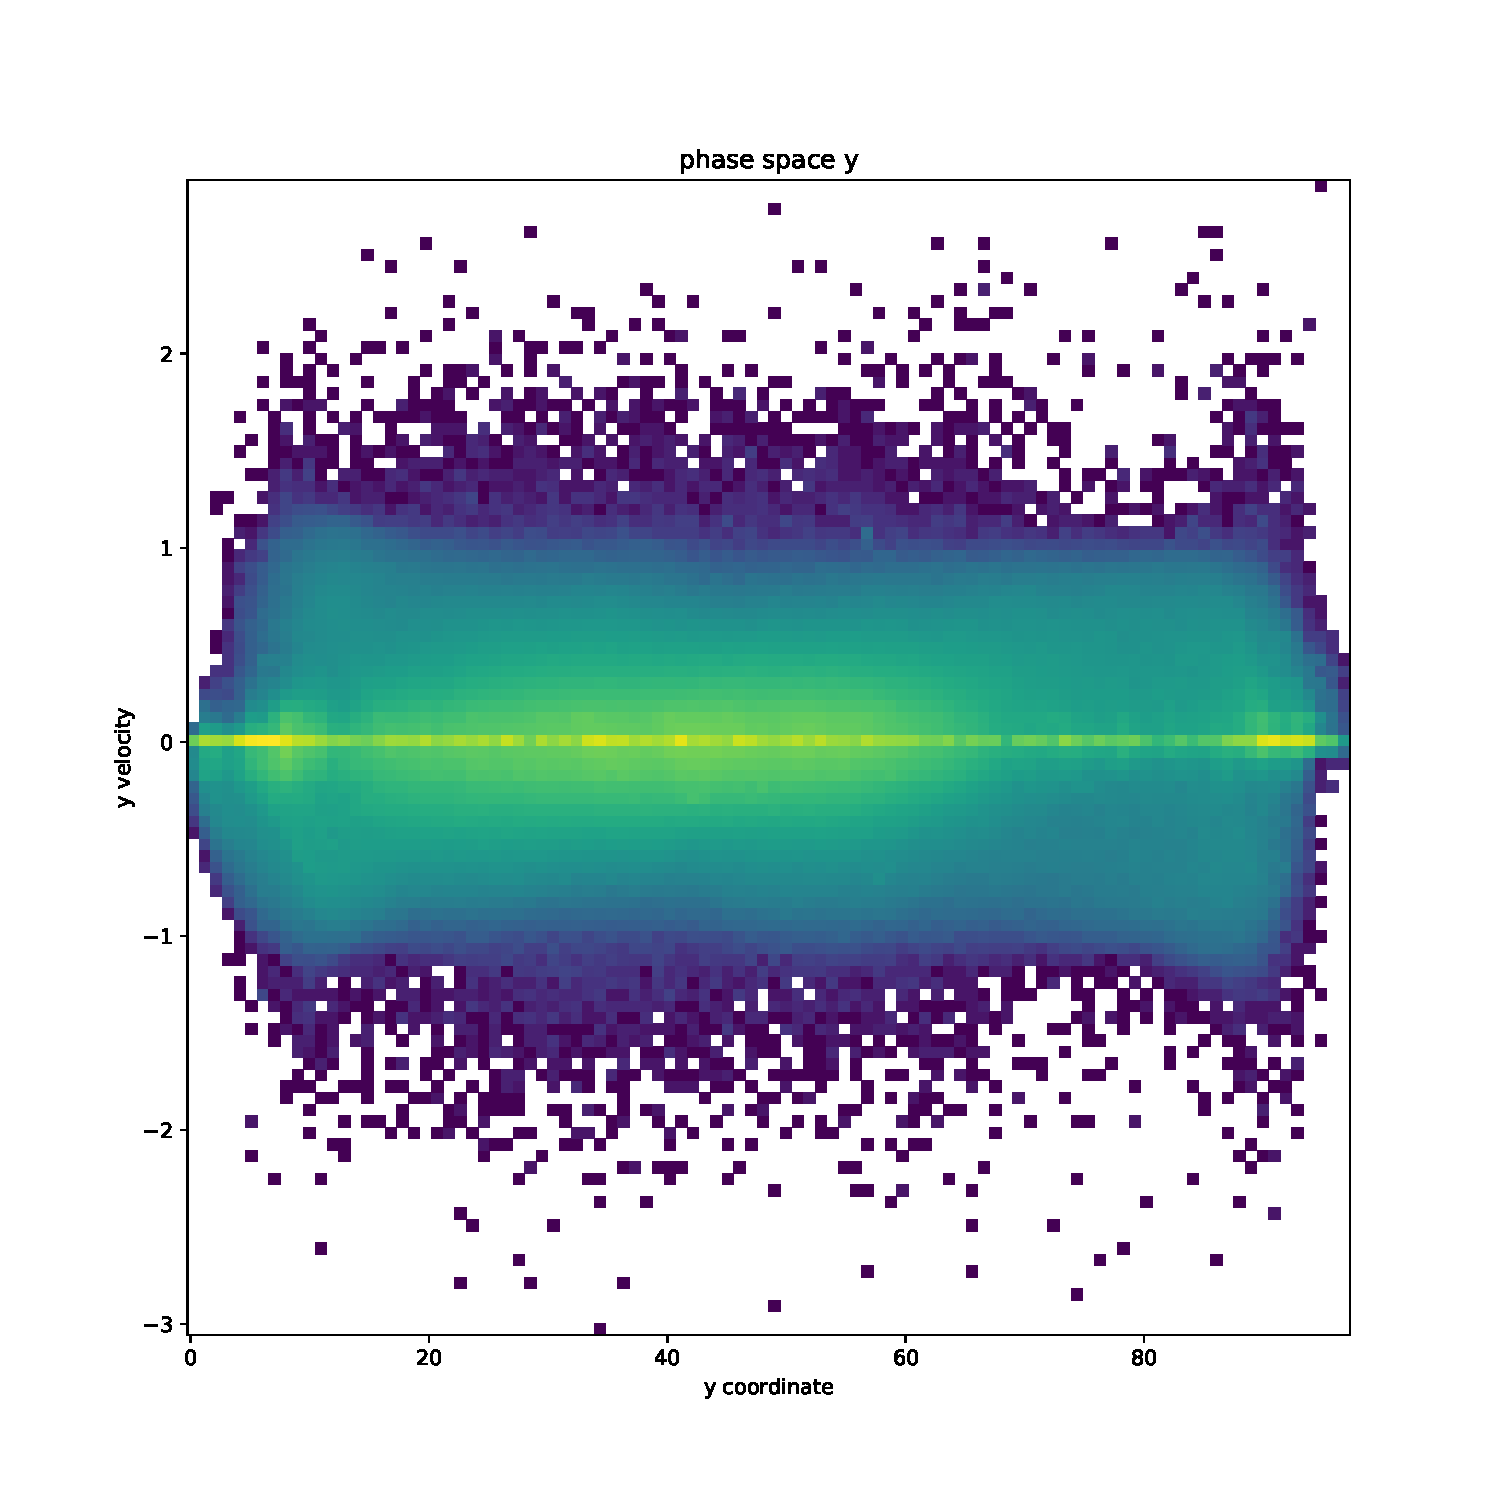
\includegraphics[ width=0.3\textwidth]{fig/hist2d_yvy/save_trainf10_pro_simTD2Q9_hist2d_y_vy}
    }
    \caption{(iii) \& (iv) - simTD2Q9 - The correlation between the position along the $\vec x$ and $\vec y$ axis and the magnitude of the velocity vector along the same correspondent axes, plotted as heat-map or 2-dimensional histograms.}
    \label{fig:hist2d_SimTD2Q9}
\end{figure}
% --------------------------------------
\begin{figure}[!htb]
    \centering
        \subfloat[(v) Real data hist2d Pxy]{
        \label{fig:Pxy_Real_v}
        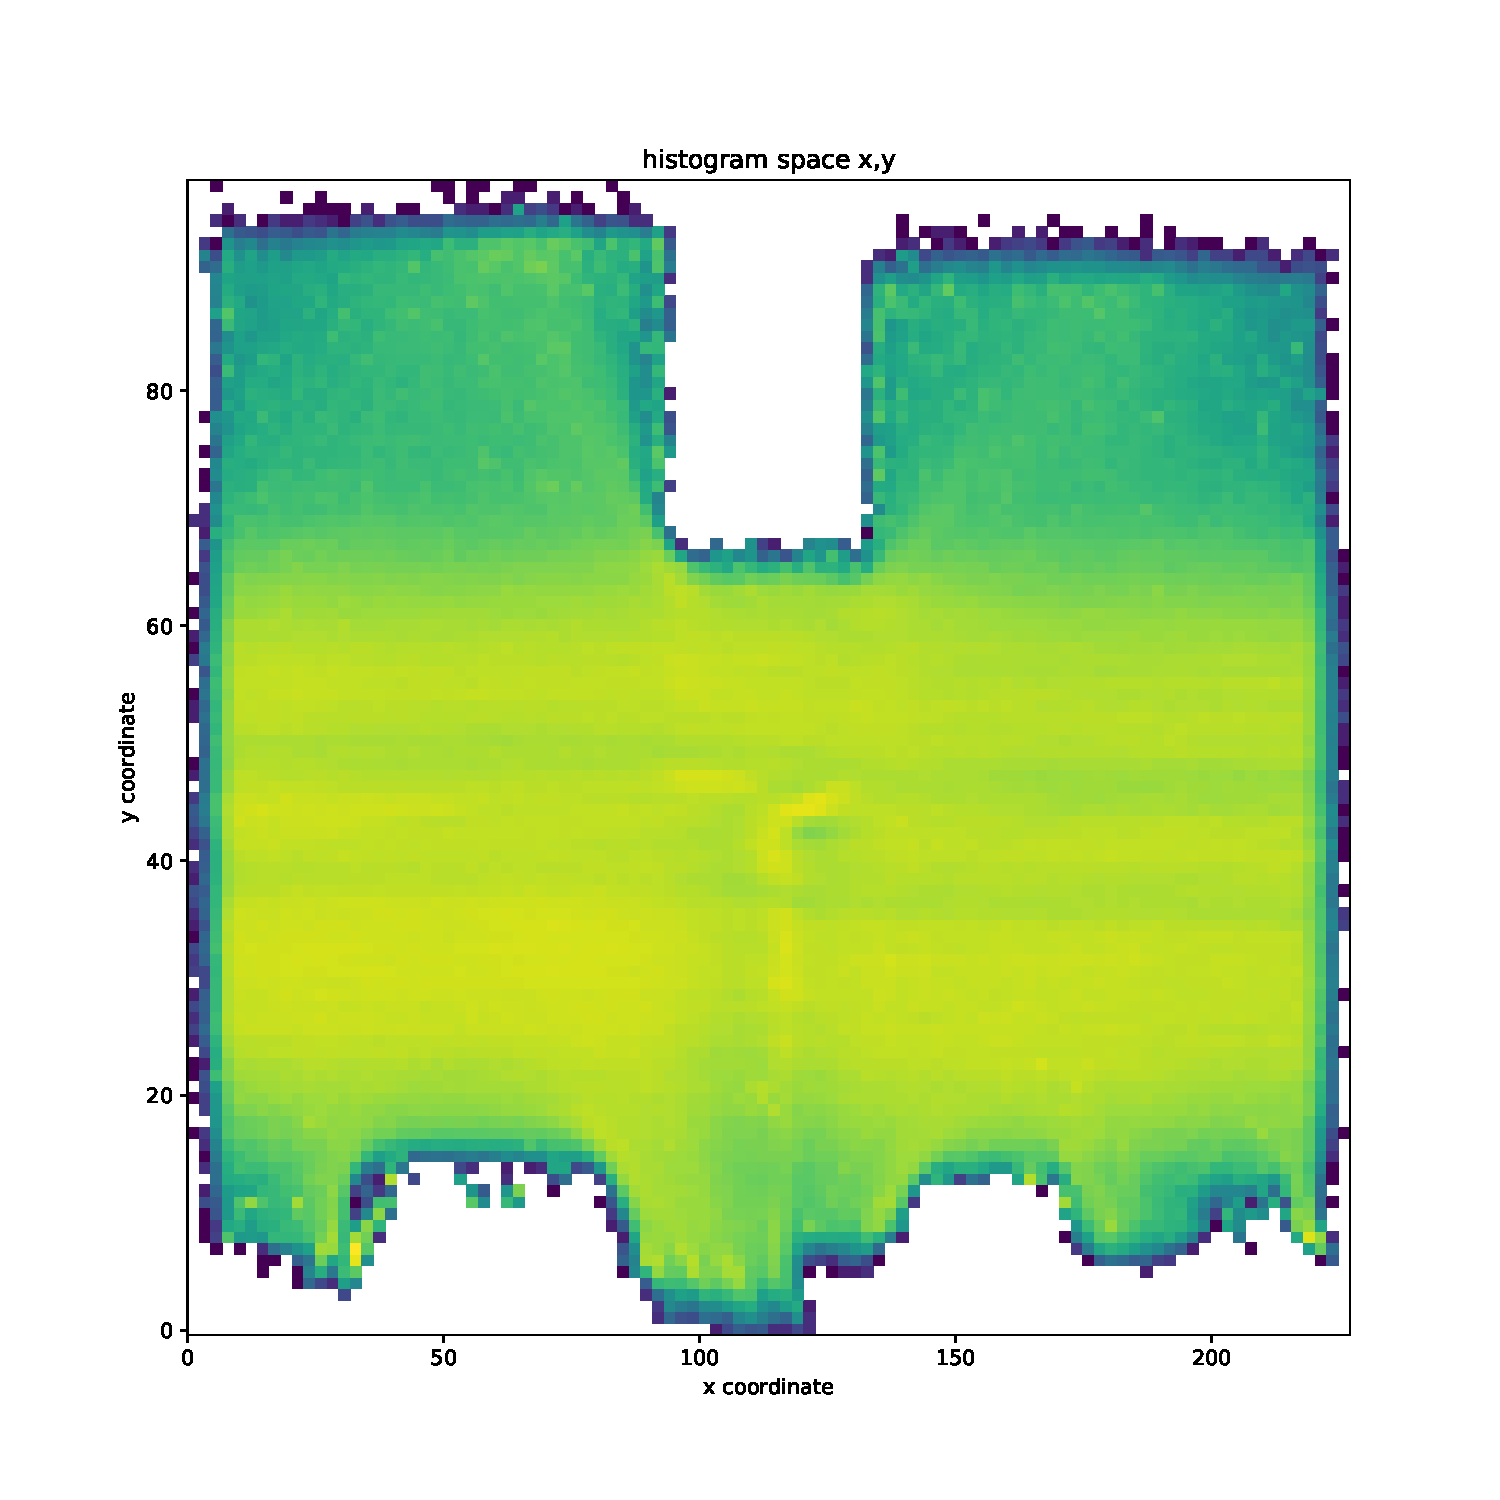
\includegraphics[ width=0.3\textwidth]{fig/hist2d_pxy/save_trainf10_pro_RealData_hist2d_x_y}
    }\quad\quad
    \subfloat[(v) Simulation data hist2d Pxy]{
        \label{fig:Pxy_SimTD2Q9}
        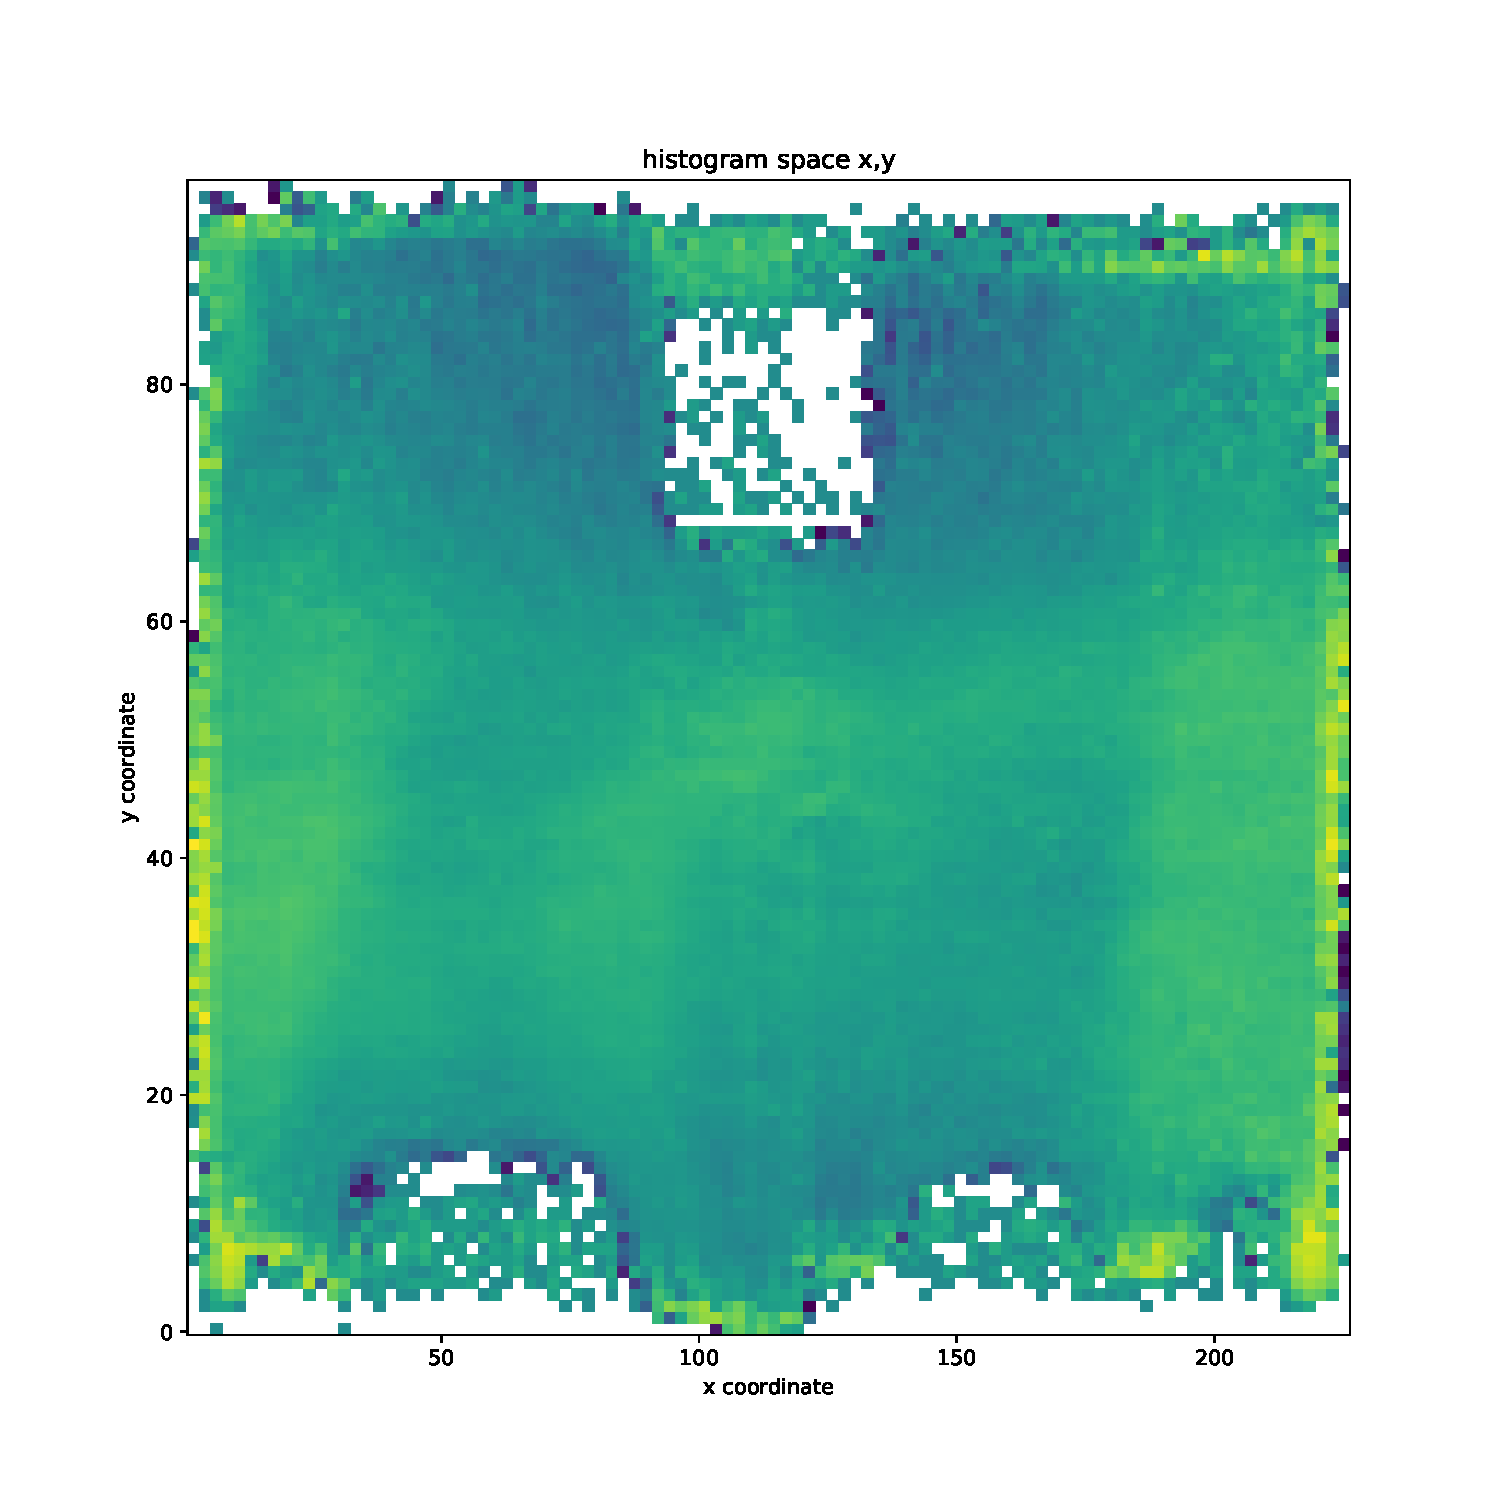
\includegraphics[ width=0.3\textwidth]{fig/hist2d_pxy/save_trainf10_pro_simTD2Q9_hist2d_x_y}
    }
    \caption{(v) - simTD2Q9 - The heat-map of the positions along $\vec x$ and $\vec y$ axis of all paths that have passed though, plotted as 2-dimensional histogram.}
    \label{fig:Pxy_SimTD2Q9}
\end{figure}


\FloatBarrier
% -------------------------------------------------------------------------------------------------------------------------------------------------------------------------------------------
\subsection{Real data - TD2Q9Q9}
This paragraph's reference are the following: (Figure \ref{fig:hist_SimTD2Q9Q9}), (Figure \ref{fig:hist2d_SimTD2Q9Q9}), (Figure \ref{fig:Pxy_SimTD2Q9Q9}) 

\begin{figure}[!htb]
    \centering
    \subfloat[(i) Real data hist vx]{
        \label{fig:Vx_Real_i}
        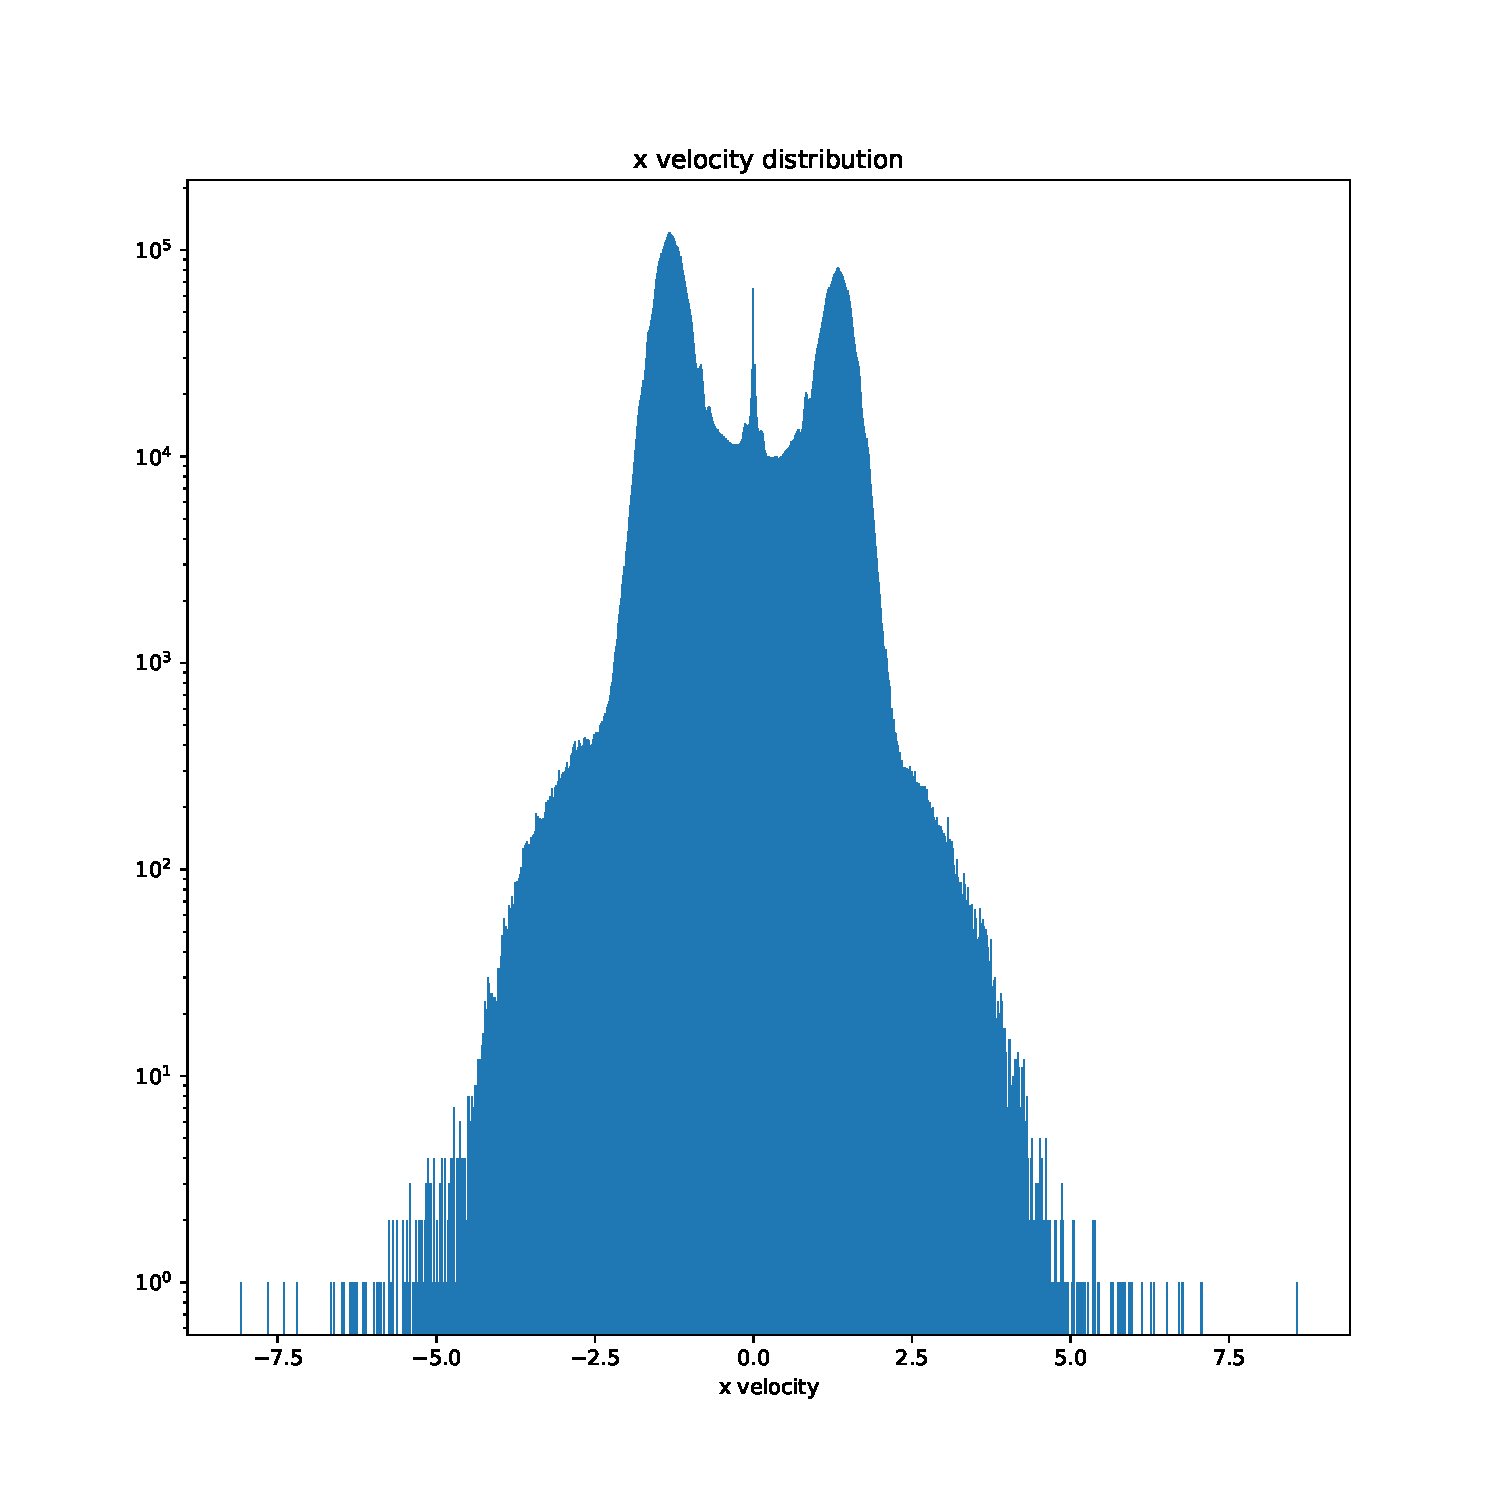
\includegraphics[ width=0.3\textwidth]{fig/hist_vx/save_trainf10_pro_RealData_hist_vx}
    }\quad\quad
    \subfloat[(i) Simulation data hist vx]{
        \label{fig:Vx_SimTD2Q9Q9}
        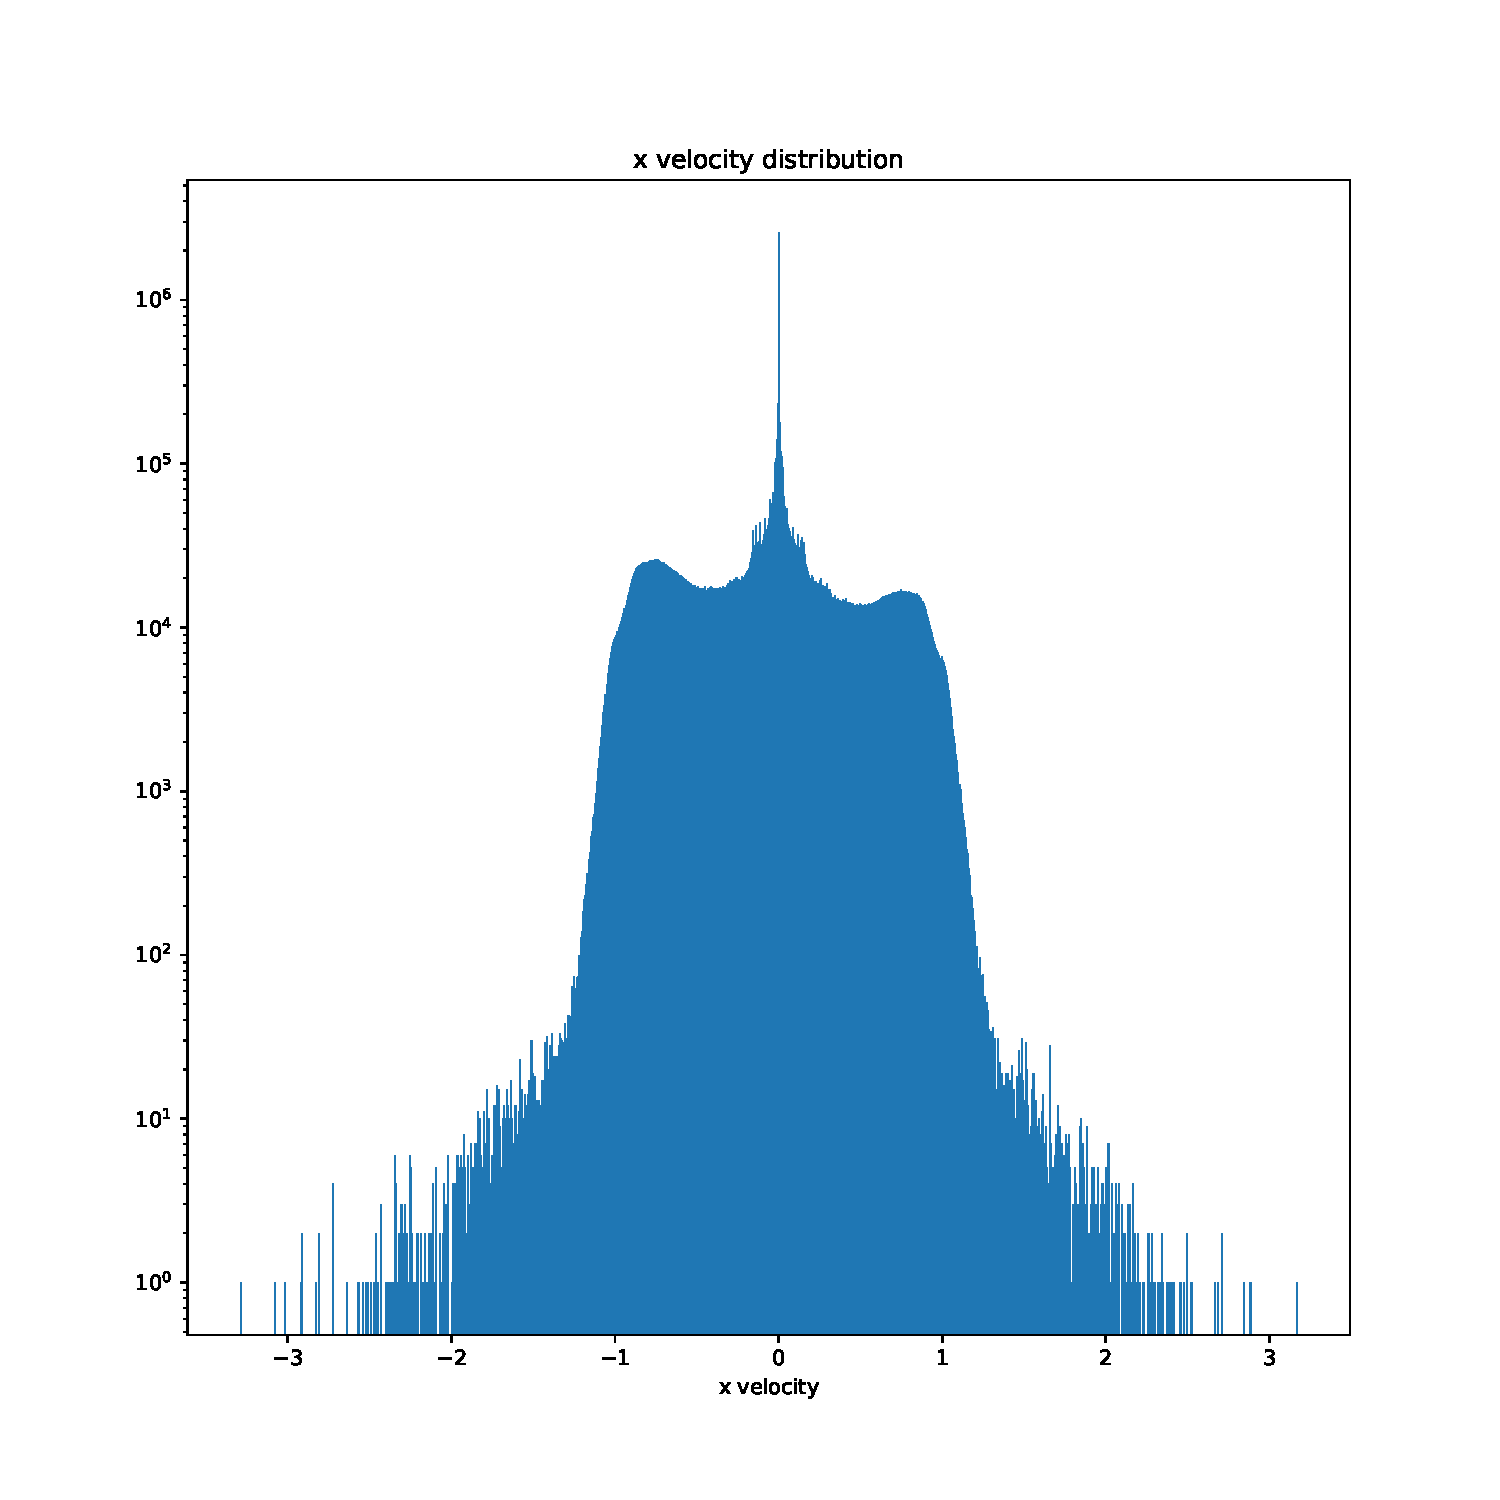
\includegraphics[ width=0.3\textwidth]{fig/hist_vx/save_trainf10_pro_simTD2Q9Q9_hist_vx}
    }\quad\quad
    \subfloat[(ii) Real data hist vy]{
        \label{fig:Vy_Real_ii}
        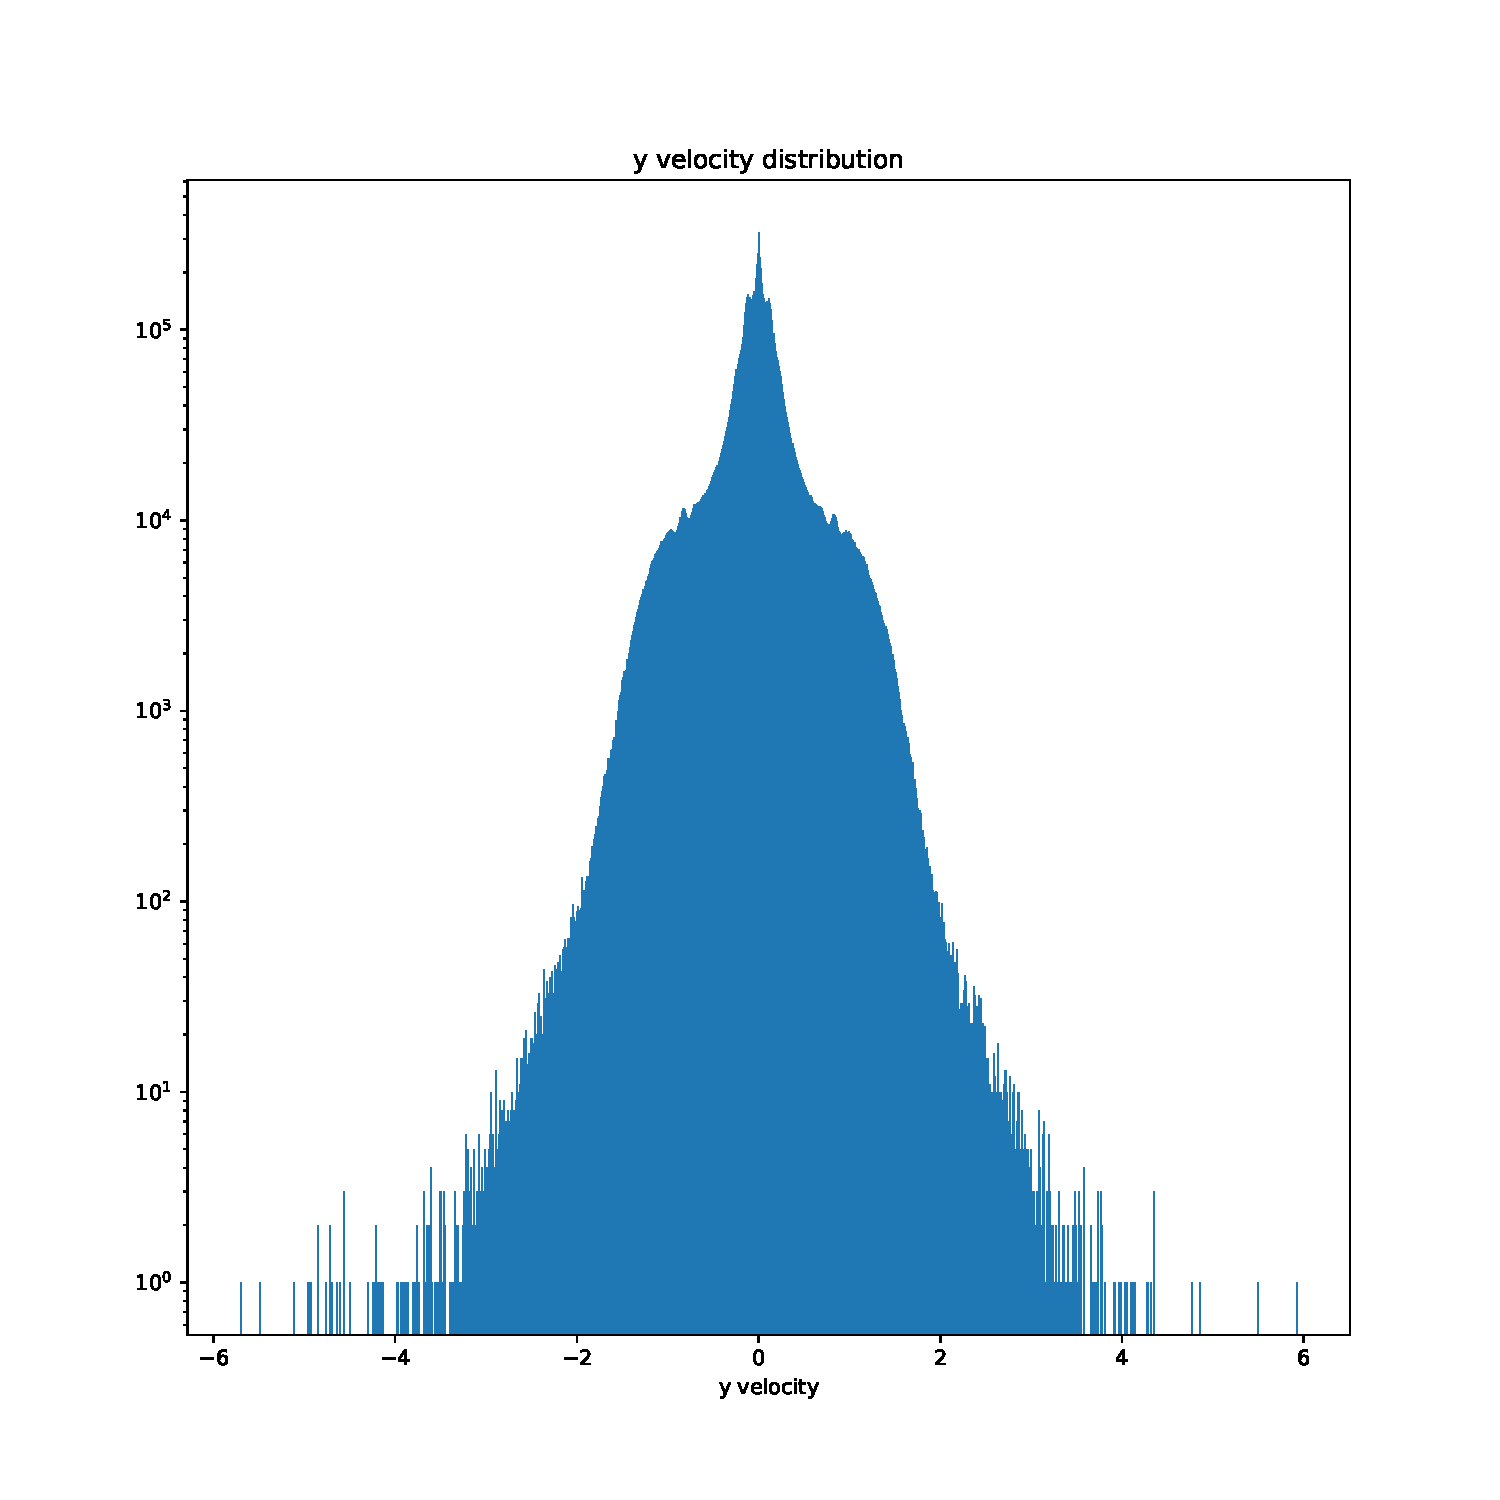
\includegraphics[ width=0.3\textwidth]{fig/hist_vy/save_trainf10_pro_RealData_hist_vy}
    }\quad\quad
    \subfloat[(ii) Simulation data hist vy]{
        \label{fig:Vy_SimTD2Q9Q9}
        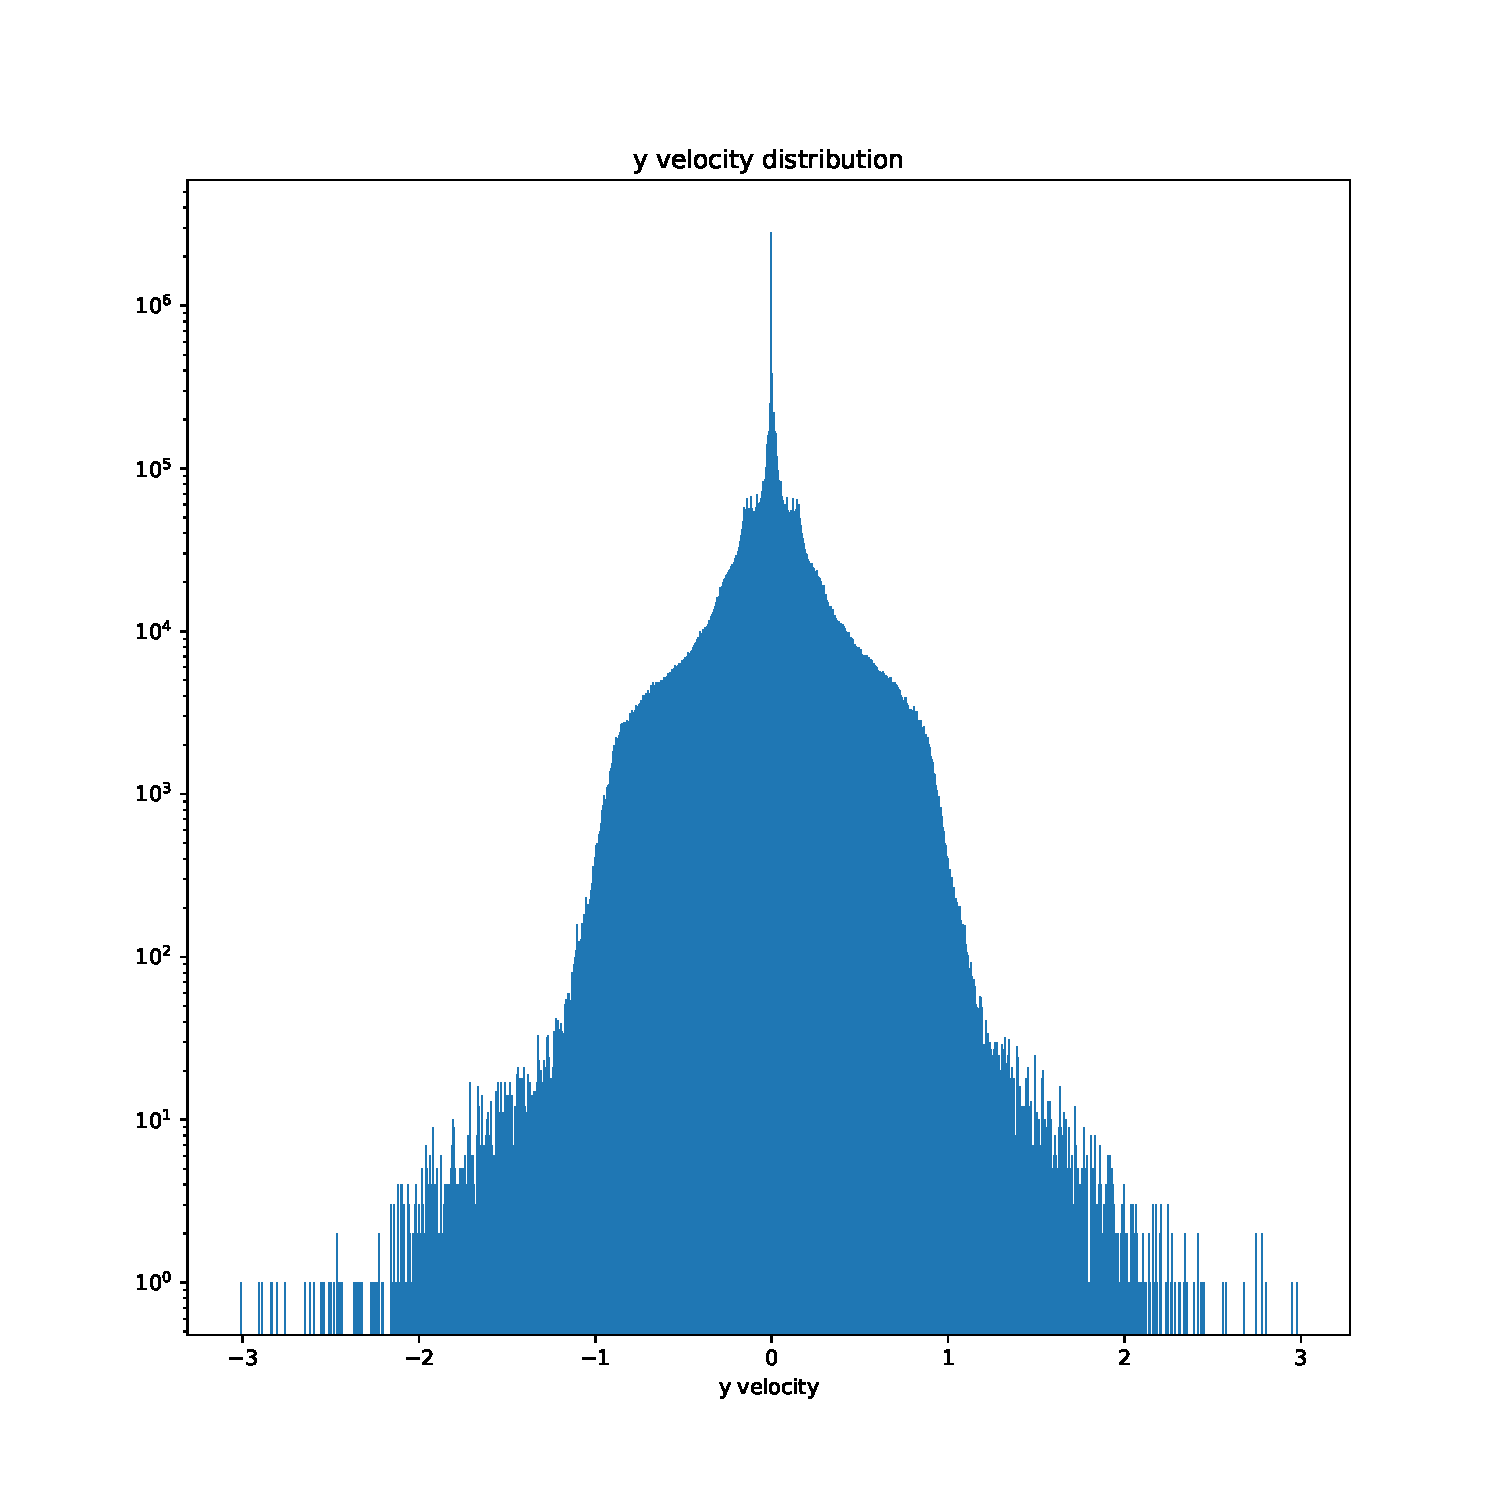
\includegraphics[ width=0.3\textwidth]{fig/hist_vy/save_trainf10_pro_simTD2Q9Q9_hist_vy}
    }
    \caption{(i) \& (ii) - simTD2Q9Q9 - The magnitude of the velocity vector along the $\vec x$ and $\vec y$ axis, plotted as 1-dimensional histograms.}
    \label{fig:hist_SimTD2Q9Q9}
\end{figure}
% --------------------------------------
\begin{figure}[!htb]
    \centering
        \subfloat[(iii) Real data hist2d xVx]{
        \label{fig:xVx_Real_iii}
        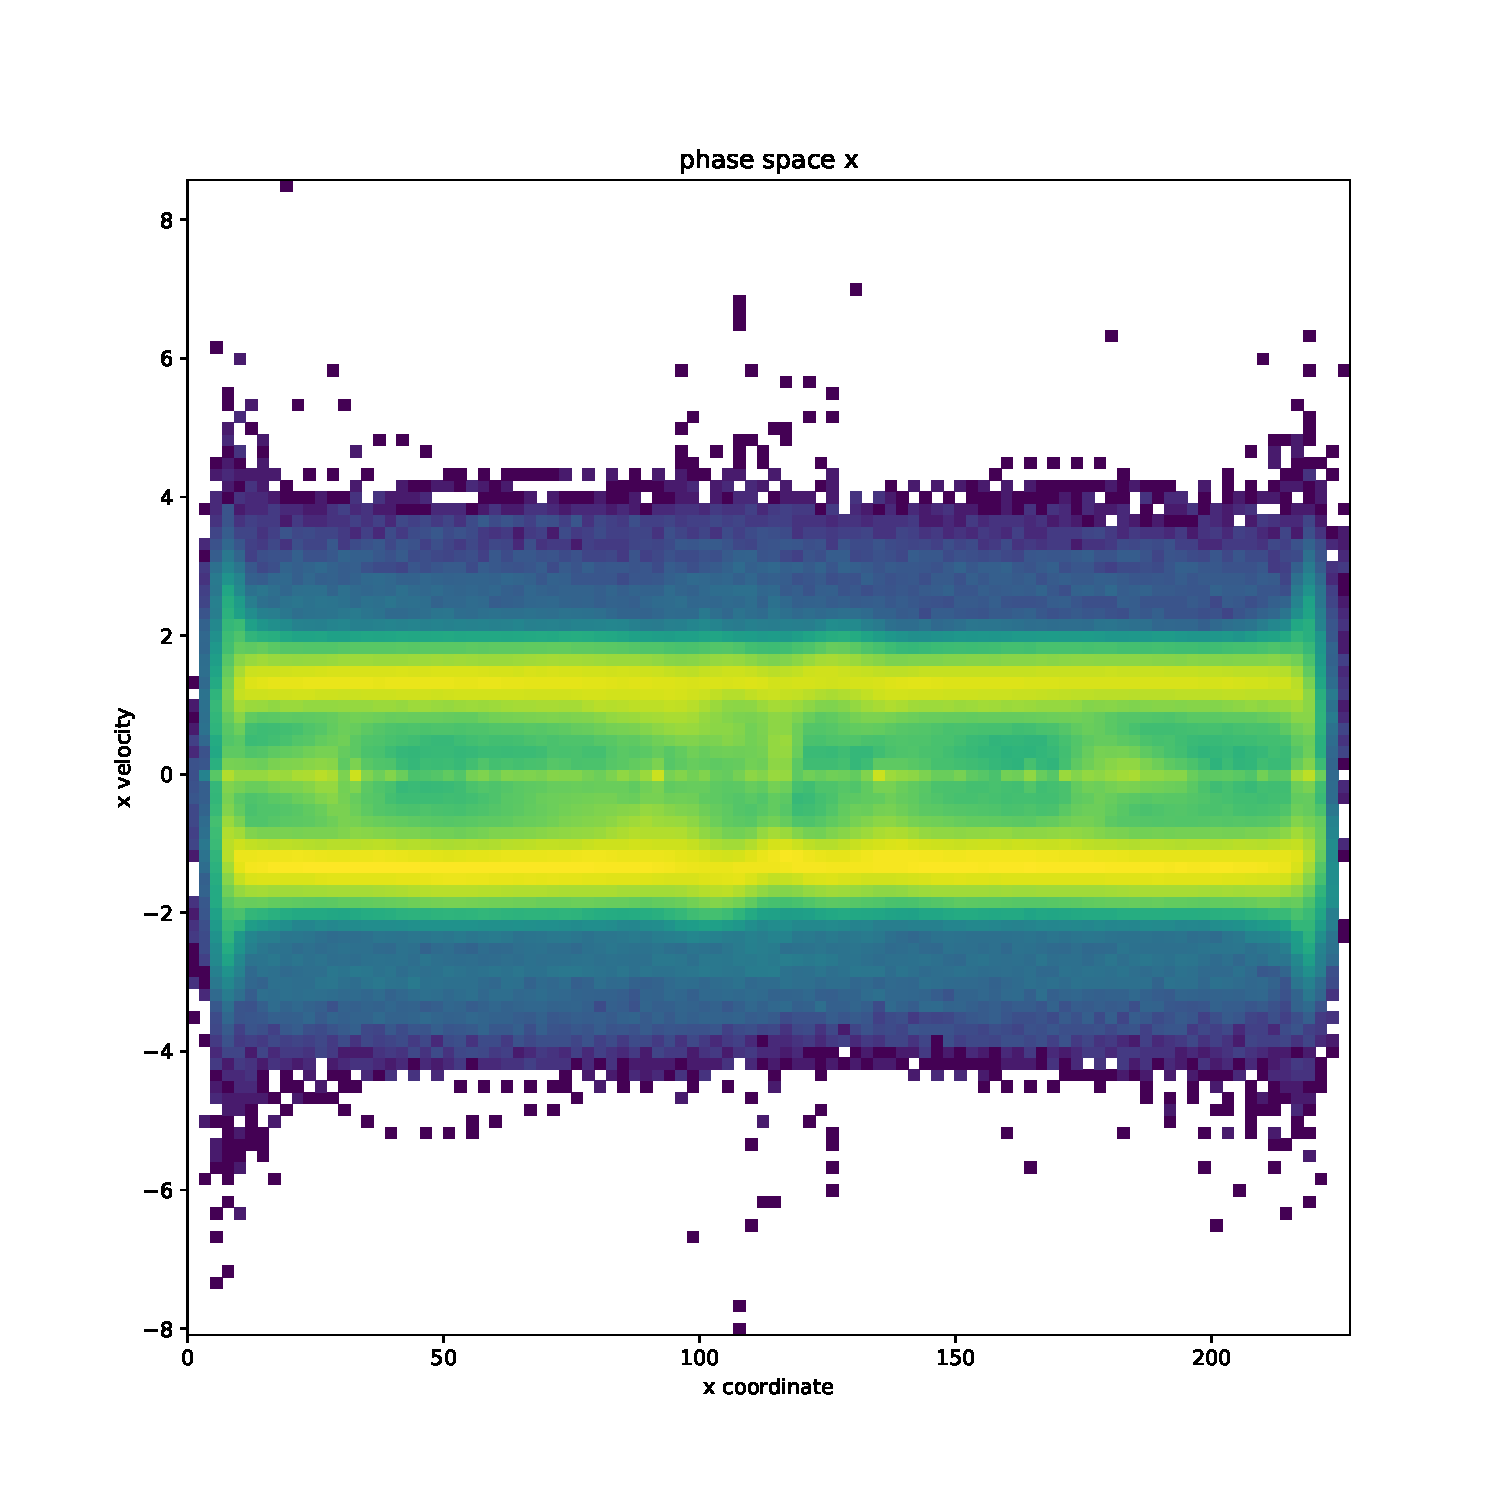
\includegraphics[ width=0.3\textwidth]{fig/hist2d_xvx/save_trainf10_pro_RealData_hist2d_x_vx}
    }\quad\quad
    \subfloat[(iii) Simulation data hist2d xVx]{
        \label{fig:xVx_SimTD2Q9Q9}
        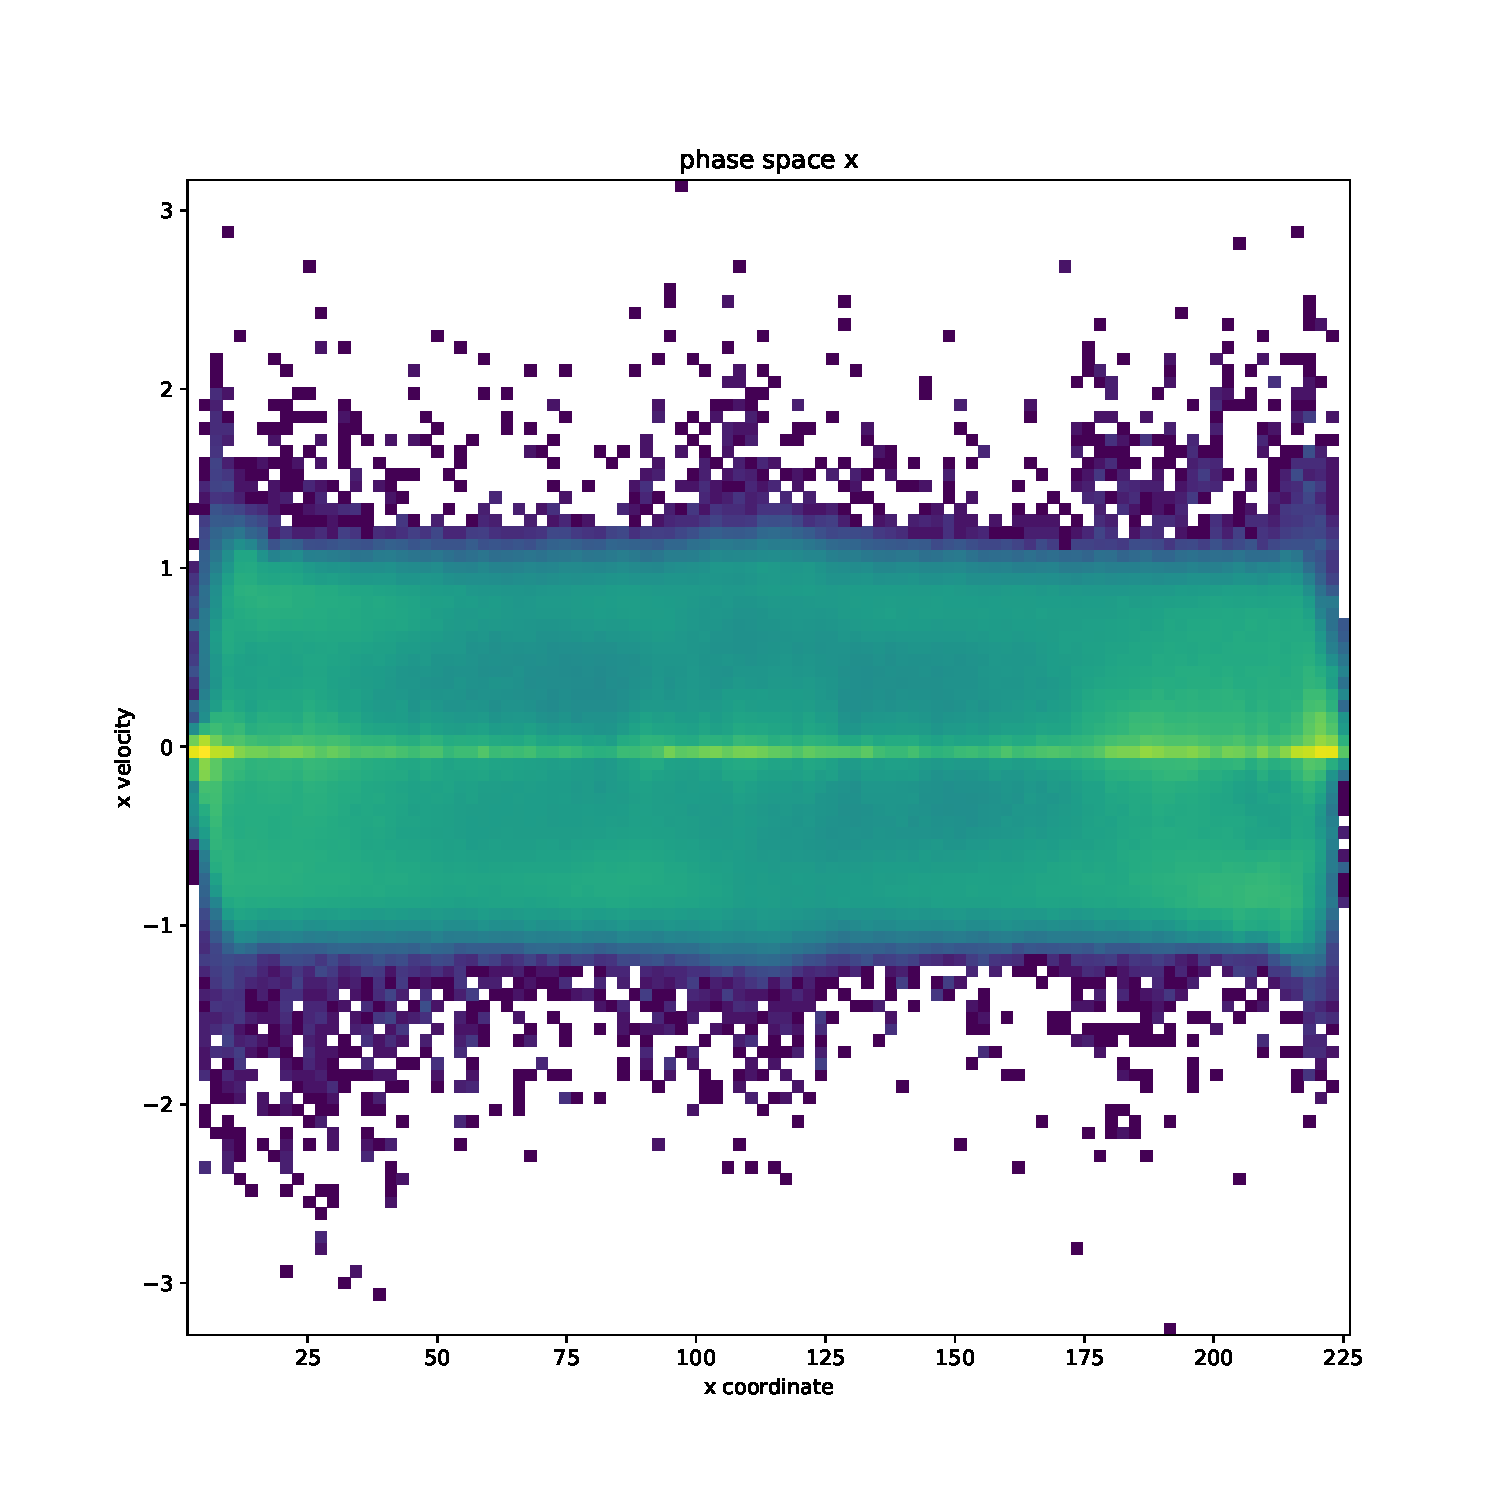
\includegraphics[ width=0.3\textwidth]{fig/hist2d_xvx/save_trainf10_pro_simTD2Q9Q9_hist2d_x_vx}
    }\quad\quad
    \subfloat[(iv) Real data hist2d yVy]{
        \label{fig:yvy_Real_iv}
        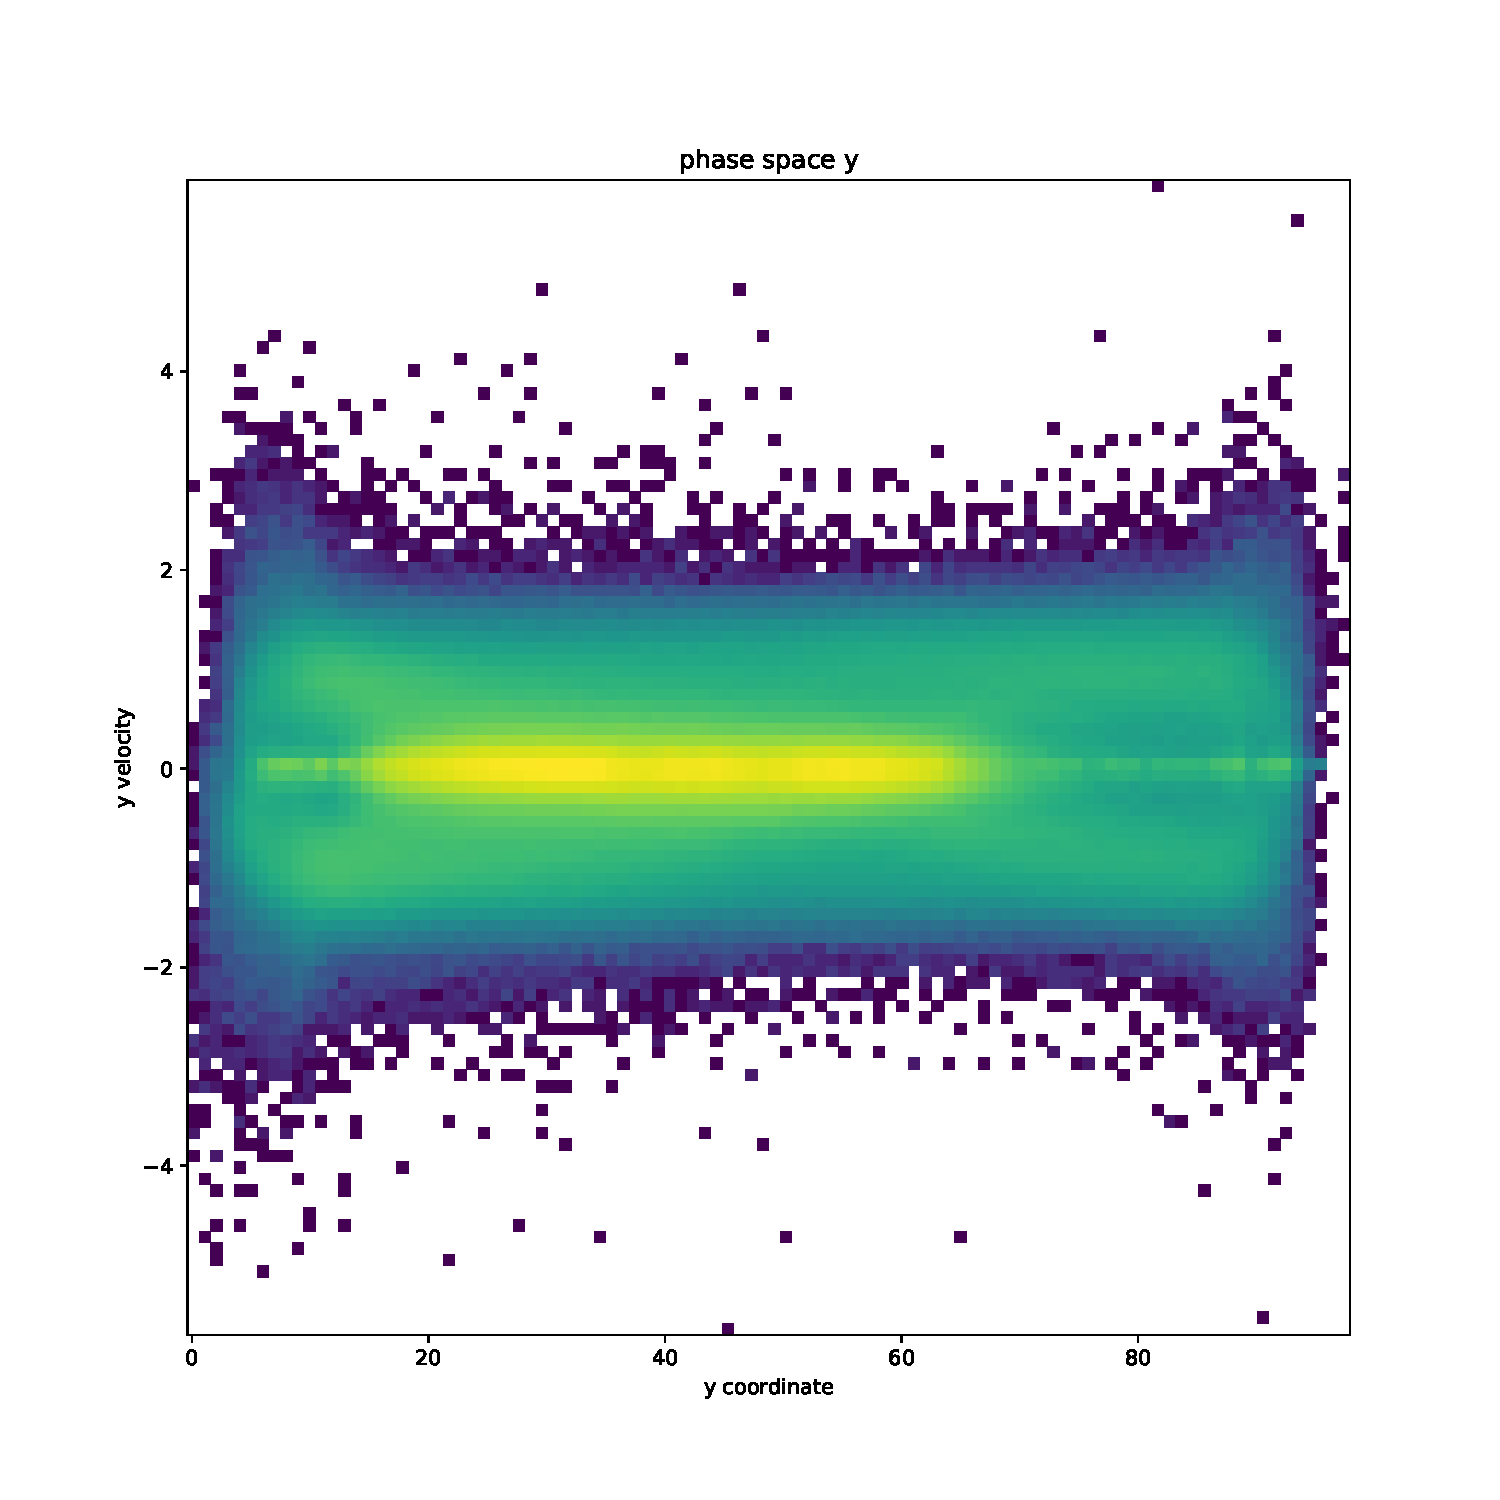
\includegraphics[ width=0.3\textwidth]{fig/hist2d_yvy/save_trainf10_pro_RealData_hist2d_y_vy}
    }\quad\quad
    \subfloat[(iv) Simulation data hist2d yVy]{
        \label{fig:yVy_SimTD2Q9Q9}
        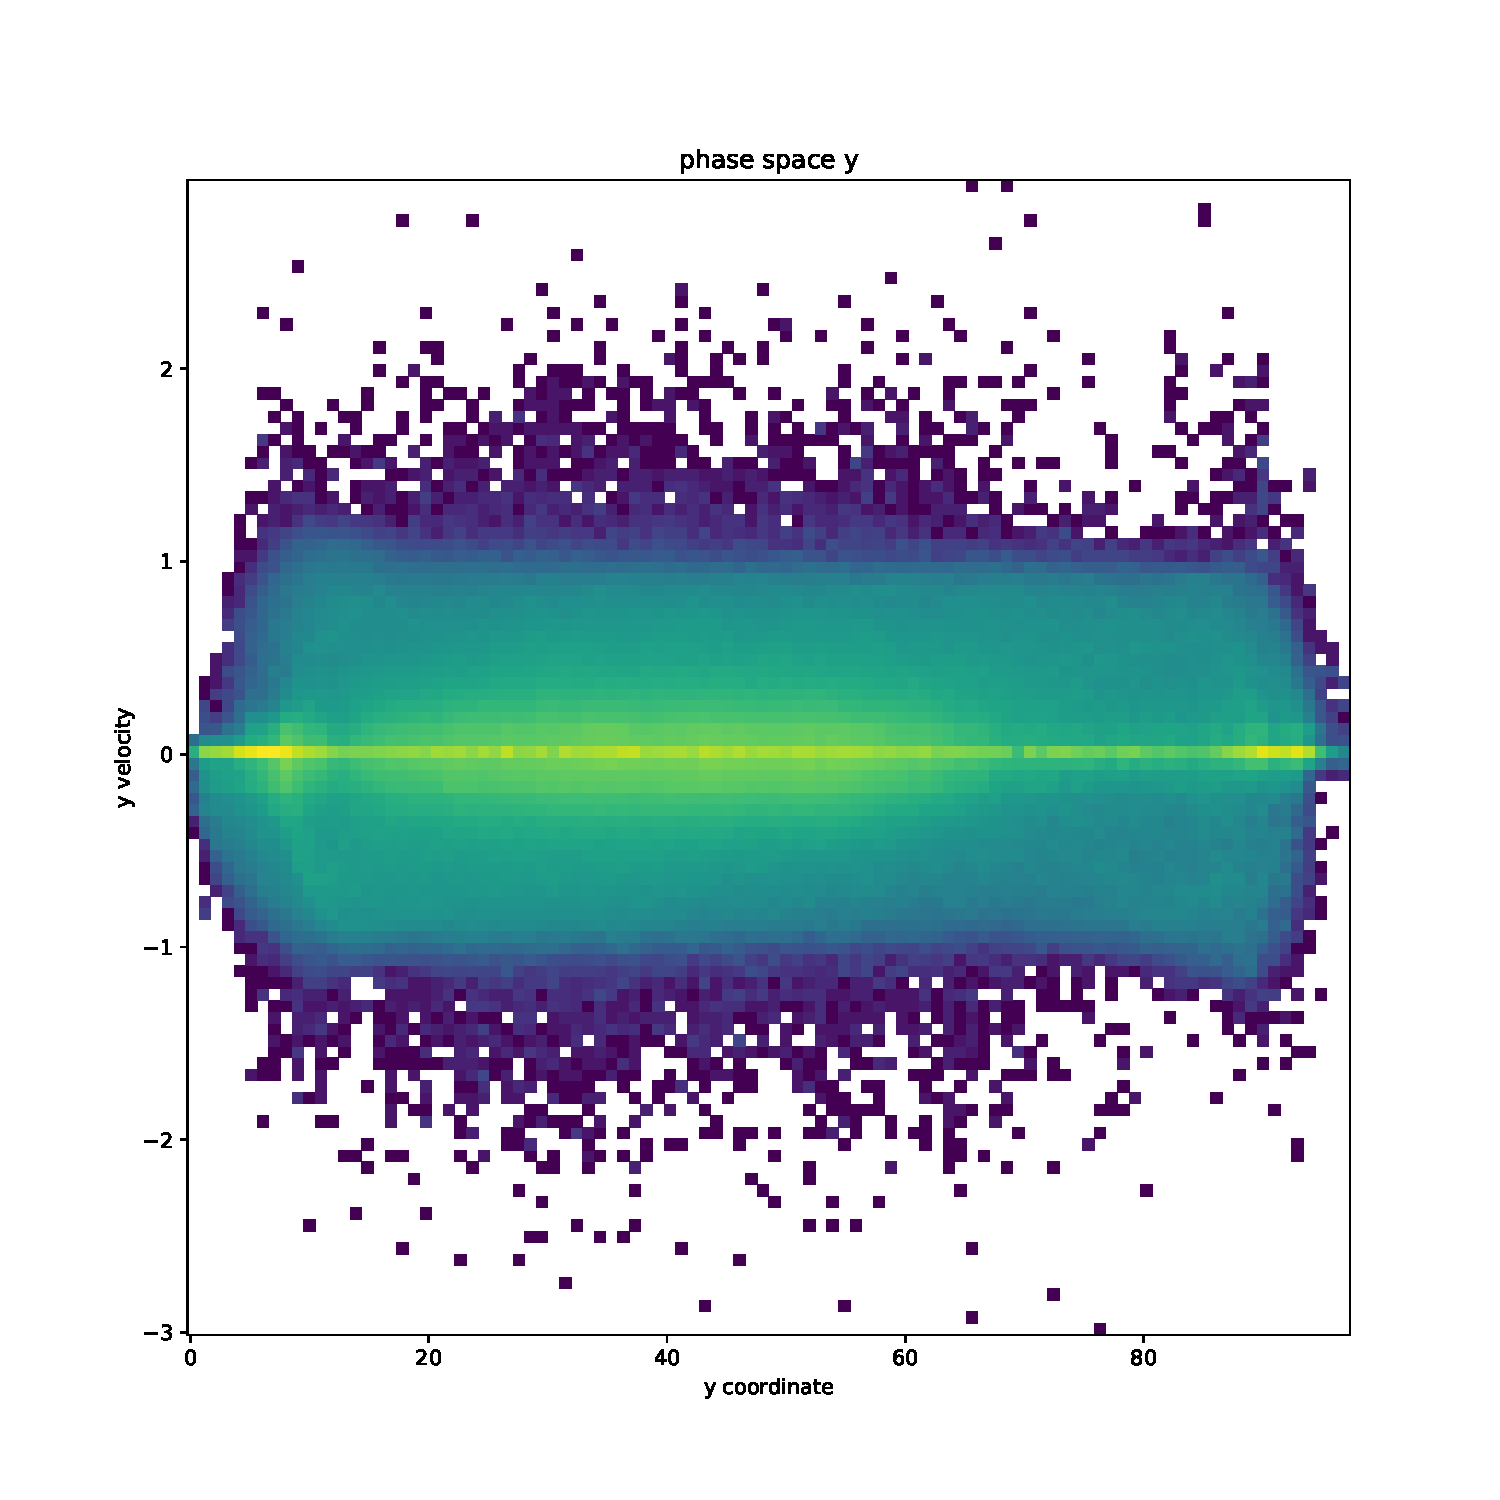
\includegraphics[ width=0.3\textwidth]{fig/hist2d_yvy/save_trainf10_pro_simTD2Q9Q9_hist2d_y_vy}
    }
    \caption{(iii) \& (iv) - simTD2Q9Q9 - The correlation between the position along the $\vec x$ and $\vec y$ axis and the magnitude of the velocity vector along the same correspondent axes, plotted as heat-map or 2-dimensional histograms.}
        \label{fig:hist2d_SimTD2Q9Q9}
\end{figure}
% --------------------------------------
\begin{figure}[!htb]
    \centering
        \subfloat[(v) Real data hist2d Pxy]{
        \label{fig:Pxy_Real_v}
        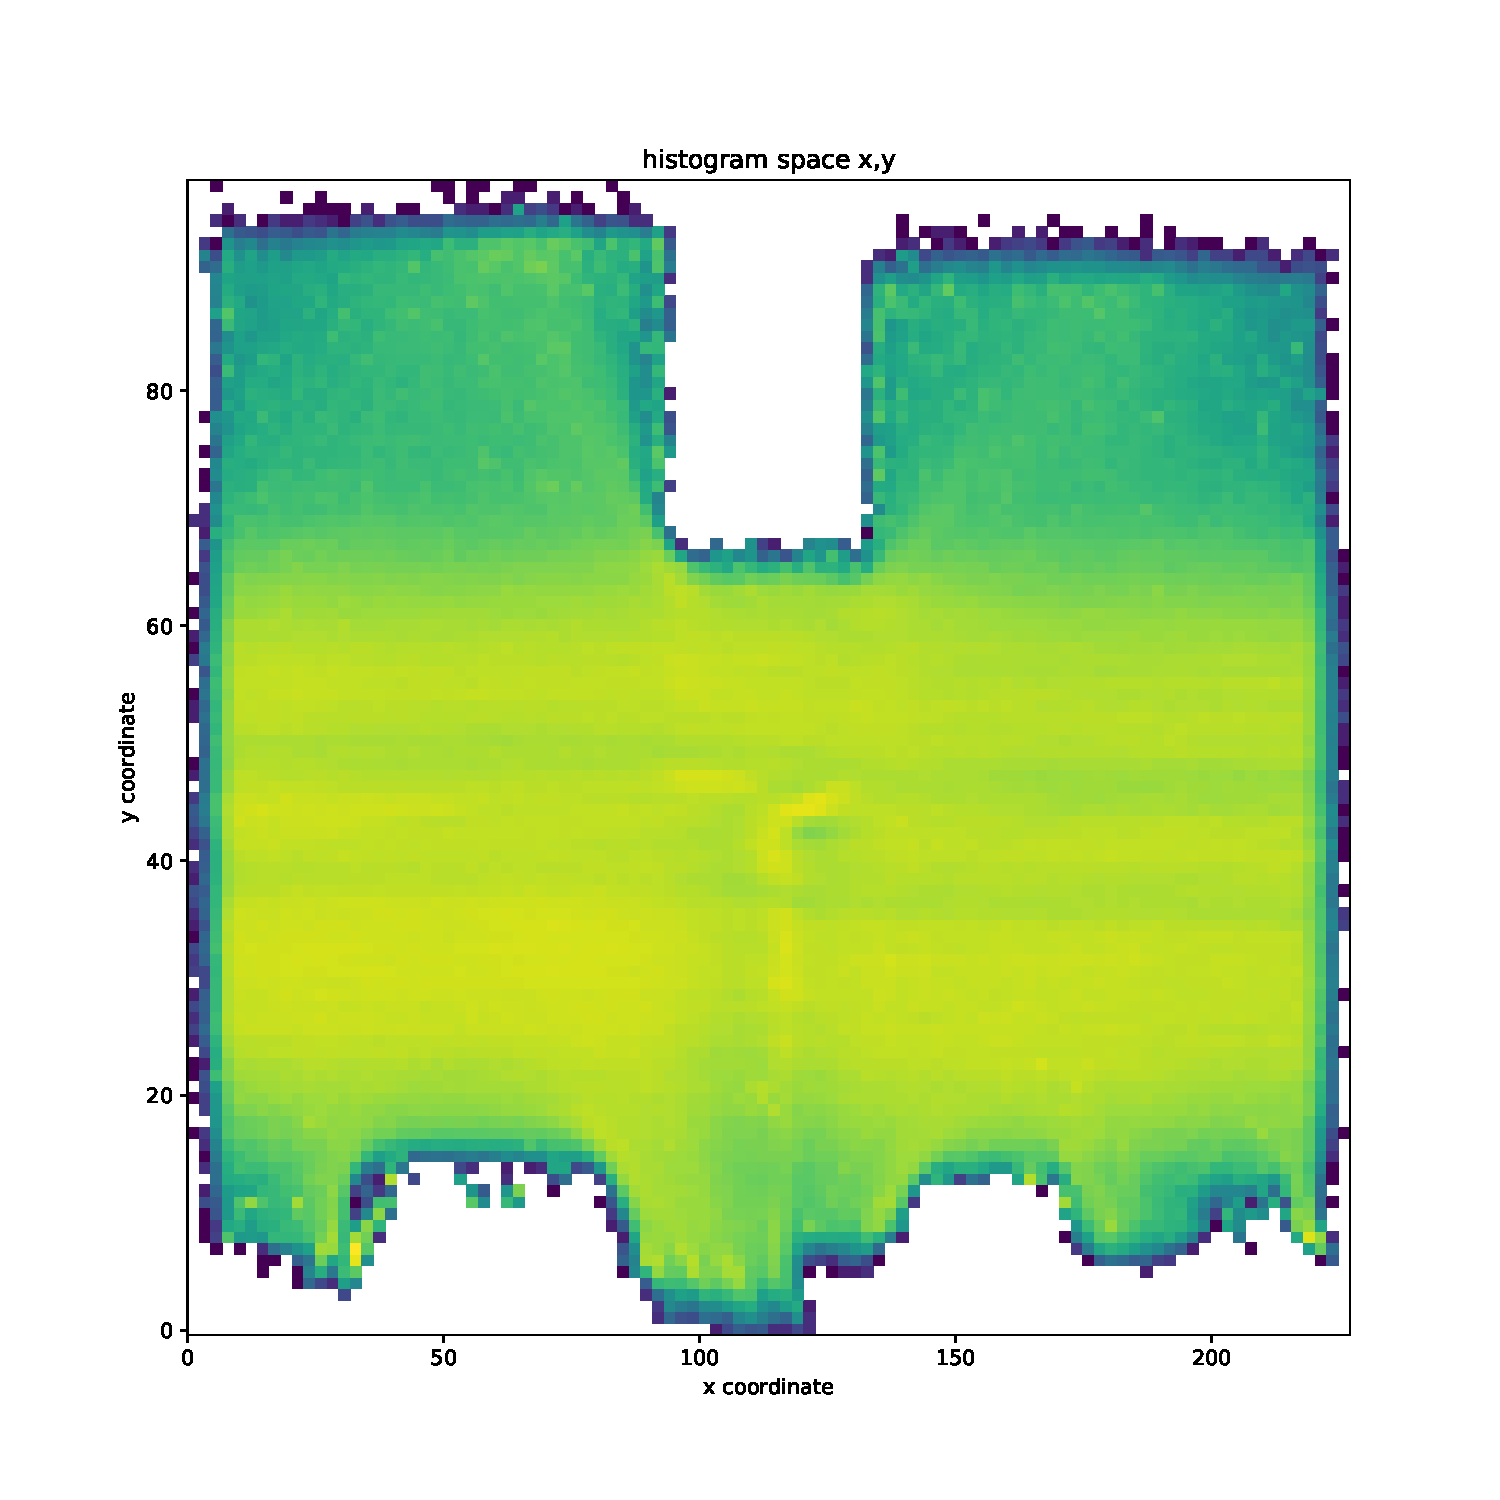
\includegraphics[ width=0.3\textwidth]{fig/hist2d_pxy/save_trainf10_pro_RealData_hist2d_x_y}
    }\quad\quad
    \subfloat[(v) Simulation data hist2d Pxy]{
        \label{fig:Pxy_SimTD2Q9Q9}
        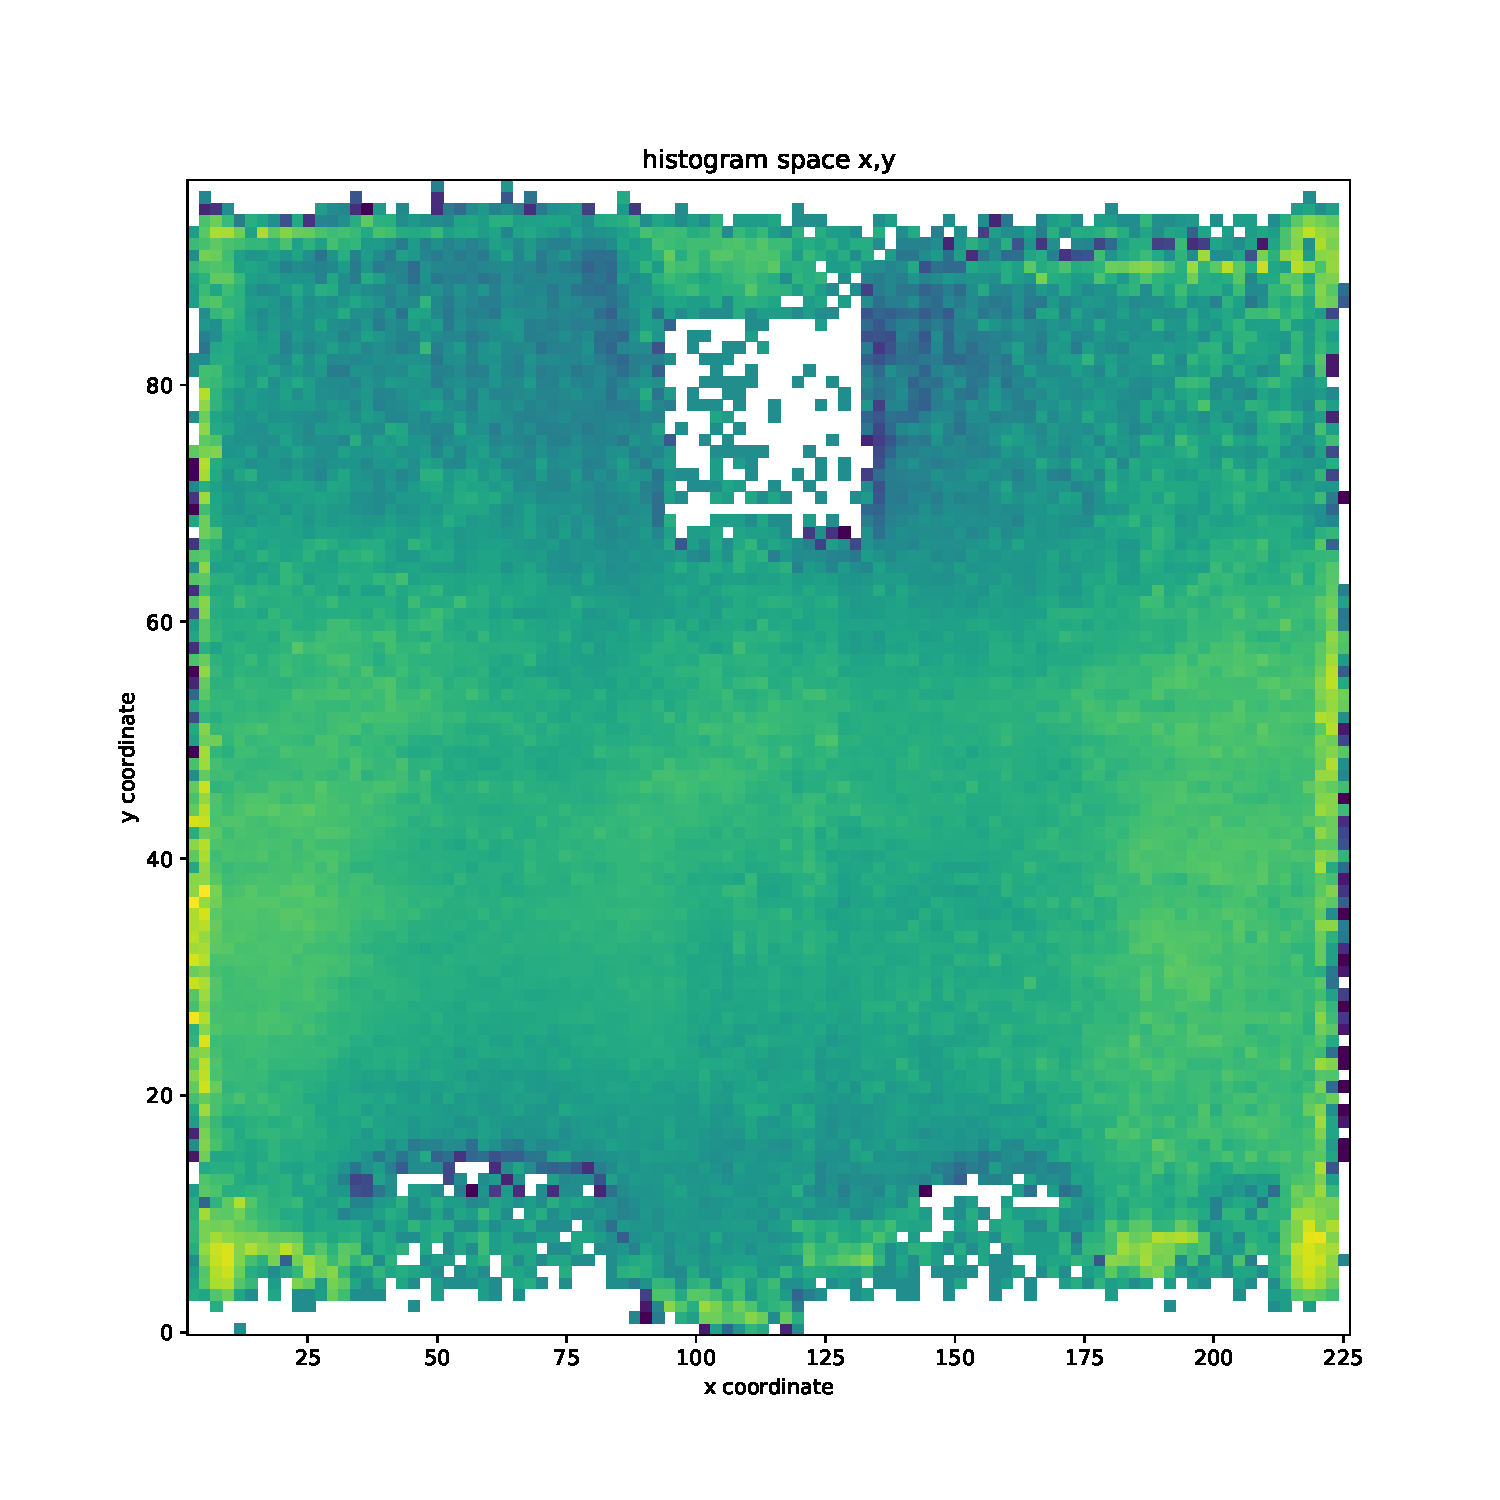
\includegraphics[ width=0.3\textwidth]{fig/hist2d_pxy/save_trainf10_pro_simTD2Q9Q9_hist2d_x_y}
    }
    \caption{(v) - simTD2Q9Q9 - The heat-map of the positions along $\vec x$ and $\vec y$ axis of all paths that have passed though, plotted as 2-dimensional histogram.}
    \label{fig:Pxy_SimTD2Q9Q9}
\end{figure}


\FloatBarrier
\end{document}
